\documentclass[11pt,a4paper,openany]{book}

% ---------------------------------------------------------------------------
% Packages
% ---------------------------------------------------------------------------
\usepackage[T1]{fontenc}
\usepackage[utf8]{inputenc}
\usepackage{lmodern}
\usepackage{microtype}
\usepackage[margin=2.5cm,headheight=14pt]{geometry}
\usepackage{amsmath,amssymb,amsfonts,bm}
\usepackage{graphicx}
\usepackage{booktabs,tabularx,longtable,array}
\usepackage{xcolor}
\usepackage{enumitem}
\usepackage{fancyhdr}
\usepackage{caption}
\usepackage{subcaption}
\usepackage{listings}
\usepackage[most]{tcolorbox}
\usepackage{tikz}
\usetikzlibrary{arrows.meta,positioning,shapes.geometric,shapes.misc,
  fit,calc,backgrounds,decorations.pathmorphing,decorations.pathreplacing,
  matrix,trees}
\usepackage{pgfplots}
\pgfplotsset{compat=1.16}
\usepackage{float}
\usepackage[hidelinks]{hyperref}

\graphicspath{{figures/}}
\renewcommand{\tabularxcolumn}[1]{>{\raggedright\arraybackslash}p{#1}}
\captionsetup{font=small,labelfont=bf}

% Walkthrough screenshots: kept in reading order, at a modest size.
\newcommand{\shot}[3][0.55]{%
  \begin{figure}[H]\centering
  \fbox{\includegraphics[width=#1\textwidth]{#2}}
  \caption{#3}\label{fig:#2}\end{figure}}
% Element-by-element description that follows each screenshot.
\newenvironment{elements}
  {\par\small\noindent\begin{tabular}{@{}>{\raggedright\arraybackslash\bfseries}p{3.4cm}
     >{\raggedright\arraybackslash}p{\dimexpr\linewidth-3.4cm-2\tabcolsep\relax}@{}}
   \toprule \textnormal{\textit{Element}} & \textit{What it shows or does}\\\midrule}
  {\bottomrule\end{tabular}\par\medskip}

% ---------------------------------------------------------------------------
% Colours and styles
% ---------------------------------------------------------------------------
\definecolor{slate}{HTML}{3B4450}
\definecolor{accent}{HTML}{2F7BD0}
\definecolor{okgreen}{HTML}{2E9A58}
\definecolor{badred}{HTML}{CC3A40}
\definecolor{warnamber}{HTML}{C48612}
\definecolor{panelgrey}{HTML}{F1F3F6}
\definecolor{linegrey}{HTML}{D3D8DE}
\definecolor{codebg}{HTML}{F5F6F8}

\lstdefinestyle{py}{
  language=Python, basicstyle=\ttfamily\small, backgroundcolor=\color{codebg},
  frame=single, rulecolor=\color{linegrey}, breaklines=true,
  keywordstyle=\color{accent}\bfseries, commentstyle=\color{gray}\itshape,
  stringstyle=\color{okgreen!70!black}, showstringspaces=false,
  columns=fullflexible, xleftmargin=4pt, xrightmargin=4pt,
  aboveskip=8pt, belowskip=8pt}
\lstdefinestyle{sh}{
  basicstyle=\ttfamily\small, backgroundcolor=\color{codebg}, frame=single,
  rulecolor=\color{linegrey}, breaklines=true, columns=fullflexible,
  showstringspaces=false, xleftmargin=4pt, xrightmargin=4pt,
  aboveskip=8pt, belowskip=8pt}
\lstset{style=py}

\newtcolorbox{note}[1][Note]{colback=accent!5,colframe=accent,
  fonttitle=\bfseries,title=#1,sharp corners=south,boxrule=0.6pt}
\newtcolorbox{warn}[1][Caution]{colback=warnamber!7,colframe=warnamber,
  fonttitle=\bfseries,title=#1,sharp corners=south,boxrule=0.6pt}
\newtcolorbox{theory}[1][Theory]{colback=okgreen!5,colframe=okgreen!70!black,
  fonttitle=\bfseries,title=#1,sharp corners=south,boxrule=0.6pt}

\newcommand{\code}[1]{\texttt{\detokenize{#1}}}
\newcommand{\tg}[1]{\textsf{\detokenize{#1}}}
\newcommand{\ui}[1]{\textbf{#1}}

% TikZ styles shared by every diagram
\tikzset{
  >={Stealth[length=2.4mm]},
  box/.style={draw=slate,rounded corners=3pt,fill=panelgrey,align=center,
    minimum height=9mm,inner sep=5pt,font=\small},
  hot/.style={box,fill=accent!12,draw=accent},
  good/.style={box,fill=okgreen!12,draw=okgreen!70!black},
  bad/.style={box,fill=badred!10,draw=badred},
  decision/.style={diamond,aspect=2.2,draw=slate,fill=warnamber!12,
    align=center,font=\small,inner sep=1pt},
  term/.style={rounded rectangle,draw=slate,fill=slate,text=white,
    font=\small\bfseries,minimum height=8mm,inner sep=6pt},
  flow/.style={->,thick,draw=slate},
  dflow/.style={->,thick,dashed,draw=slate!70},
  lbl/.style={font=\footnotesize,fill=white,inner sep=1.5pt},
}

\pagestyle{fancy}
\fancyhf{}
\fancyhead[LE,RO]{\thepage}
\fancyhead[RE]{\small\leftmark}
\fancyhead[LO]{\small\rightmark}
\renewcommand{\headrulewidth}{0.4pt}

\setlist{itemsep=2pt,topsep=4pt}
\raggedbottom
\setlength{\emergencystretch}{3em}
\setcounter{tocdepth}{1}

\title{\Huge\bfseries pyplant\\[6pt]
  \Large A two-tank process plant with its control, SCADA and\\
  fault-diagnosis stack, in Python\\[18pt]
  \large User Manual and Technical Reference}
\author{pyplant project}
\date{Version 0.1.0 \,--\, October 2026}

\begin{document}
\frontmatter
\maketitle
\tableofcontents

\mainmatter
\chapter{Introduction}
\label{ch:intro}

\section{What pyplant is}

\textbf{pyplant} is a complete, simulated industrial control system for a
small process plant, written entirely in Python. It contains every layer a
real installation has, from the physics at the bottom to a data-driven fault
diagnosis service at the top:

\begin{itemize}
  \item a \emph{physics simulator} of two gravity-drained tanks fed by a
        centrifugal pump through a control valve;
  \item a \emph{soft PLC} with a deterministic scan cycle, a velocity-form PID
        controller, alarms and a latched pump interlock;
  \item a \emph{field network} using Modbus TCP between the plant and the PLC;
  \item an \emph{OPC UA server} that publishes every signal with engineering
        units and ranges;
  \item a \emph{historian} that stores samples in DuckDB and answers
        step-hold window queries;
  \item an \emph{operator HMI} with a mimic diagram, trends and an
        ISA-18.2 alarm list;
  \item a \emph{fault injection layer} and a \emph{scenario runner} that
        produce perfectly labelled datasets;
  \item a \emph{machine-learning toolbox} with four anomaly detectors, from
        z-score limits to a neural autoencoder, evaluated with operator-facing
        metrics;
  \item the \emph{workbench}: one web page that drives all of the above.
\end{itemize}

Nothing requires hardware or vendor software. Every number in this manual can
be reproduced on a laptop.

\section{Who this manual is for}

The manual serves three audiences, and each chapter says which one it is
written for.

\begin{description}
  \item[Users] who want to run the plant, break it and train a detector.
        Read Chapters~\ref{ch:install}, \ref{ch:workbench} and
        \ref{ch:tutorials}.
  \item[Students] of control, automation or machine learning who want the
        theory behind each layer. Chapters~\ref{ch:plant} to \ref{ch:eval}
        derive every model and algorithm the code implements.
  \item[Developers] who want to change parameters, add a tag, a fault or a
        detection method. Chapters~\ref{ch:params} to \ref{ch:api}.
\end{description}

\section{The process in one picture}

Figure~\ref{fig:pid} is the piping and instrumentation view of the plant. A
pump (\tg{PMP101}) delivers water through an equal-percentage control valve
(\tg{FCV101}) into tank~1. Tank~1 drains by gravity through an orifice into
tank~2, which drains to atmosphere. The level controller \tg{LIC101} holds the
level in tank~1 (\tg{LT101}) at its setpoint by moving the valve. Tank~2 is not
controlled, so disturbances in tank~1 reach it with a lag, which is useful for
diagnosis.

\begin{figure}[htbp]
\centering
\scalebox{0.8}{%
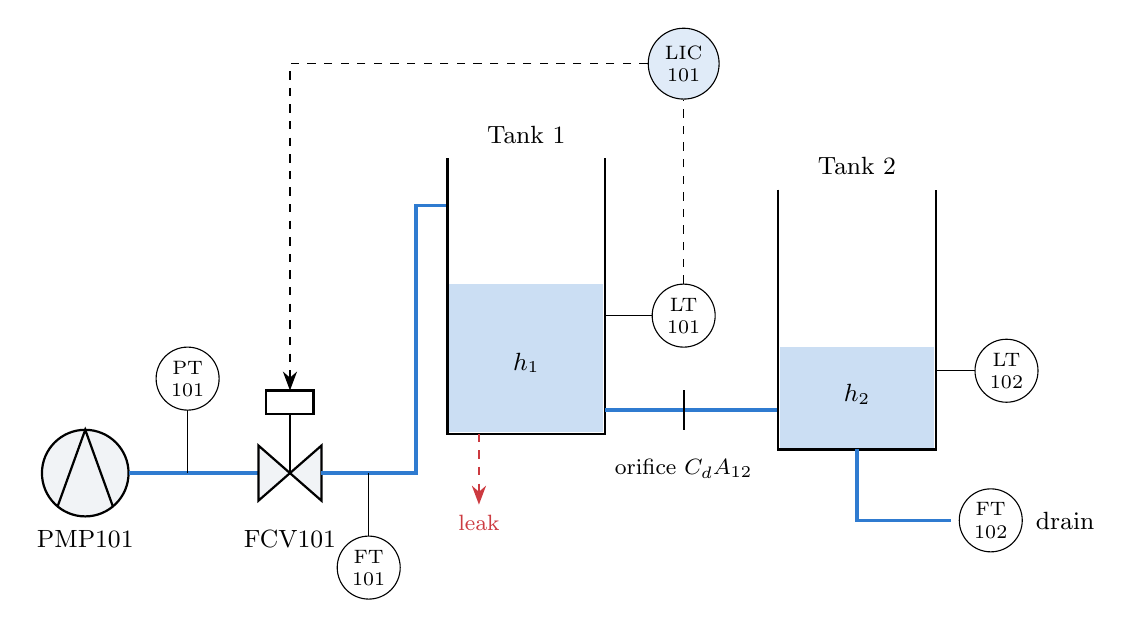
\begin{tikzpicture}[scale=1,every node/.style={font=\small}]
  % pump
  \draw[thick,fill=panelgrey] (0,0) circle (0.55);
  \draw[thick] (-0.35,-0.42) -- (0,0.55) -- (0.35,-0.42);
  \node[below=6mm] at (0,0) {PMP101};
  % pipe to valve
  \draw[very thick,accent] (0.55,0) -- (2.2,0);
  % valve (bowtie)
  \draw[thick,fill=panelgrey] (2.2,-0.35) -- (3.0,0.35) -- (3.0,-0.35) -- (2.2,0.35) -- cycle;
  \draw[thick] (2.6,0) -- (2.6,0.75);
  \draw[thick,fill=white] (2.3,0.75) rectangle (2.9,1.05);
  \node[below=4mm] at (2.6,-0.2) {FCV101};
  \draw[very thick,accent] (3.0,0) -- (4.2,0) -- (4.2,3.4) -- (4.6,3.4);
  % instruments on the discharge
  \draw (1.3,0) -- (1.3,0.8);
  \node[circle,draw,align=center,inner sep=0pt,minimum size=8mm,fill=white] at (1.3,1.2) {\scriptsize PT\\[-3pt]\scriptsize 101};
  \draw (3.6,0) -- (3.6,-0.8);
  \node[circle,draw,align=center,inner sep=0pt,minimum size=8mm,fill=white] at (3.6,-1.2) {\scriptsize FT\\[-3pt]\scriptsize 101};
  % tank 1
  \draw[thick] (4.6,4) -- (4.6,0.5) -- (6.6,0.5) -- (6.6,4);
  \fill[accent!25] (4.62,0.52) rectangle (6.58,2.4);
  \node at (5.6,4.3) {Tank 1};
  \node at (5.6,1.4) {$h_1$};
  % LT101 and controller
  \draw (6.6,2.0) -- (7.2,2.0);
  \node[circle,draw,align=center,inner sep=0pt,minimum size=8mm,fill=white] (lt) at (7.6,2.0) {\scriptsize LT\\[-3pt]\scriptsize 101};
  \node[circle,draw,align=center,inner sep=0pt,minimum size=9mm,fill=accent!15] (lic) at (7.6,5.2) {\scriptsize LIC\\[-3pt]\scriptsize 101};
  \draw[dashed] (lt) -- (lic);
  \draw[dashed,->] (lic) -| (2.6,1.05);
  % orifice to tank 2
  \draw[very thick,accent] (6.6,0.8) -- (8.8,0.8);
  \draw[thick] (7.6,0.55) -- (7.6,1.05);
  \node[below=3mm] at (7.6,0.6) {\footnotesize orifice $C_dA_{12}$};
  % tank 2
  \draw[thick] (8.8,3.6) -- (8.8,0.3) -- (10.8,0.3) -- (10.8,3.6);
  \fill[accent!25] (8.82,0.32) rectangle (10.78,1.6);
  \node at (9.8,3.9) {Tank 2};
  \node at (9.8,1.0) {$h_2$};
  \draw (10.8,1.3) -- (11.3,1.3);
  \node[circle,draw,align=center,inner sep=0pt,minimum size=8mm,fill=white] at (11.7,1.3) {\scriptsize LT\\[-3pt]\scriptsize 102};
  % drain
  \draw[very thick,accent] (9.8,0.3) -- (9.8,-0.6) -- (11.0,-0.6);
  \node[circle,draw,align=center,inner sep=0pt,minimum size=8mm,fill=white] at (11.5,-0.6) {\scriptsize FT\\[-3pt]\scriptsize 102};
  \node[right] at (11.95,-0.6) {drain};
  % leak
  \draw[->,badred,thick,dashed] (5.0,0.5) -- (5.0,-0.4) node[below] {\footnotesize leak};
\end{tikzpicture}}
\caption{Process and instrumentation of the two-tank plant. Solid blue lines
are piping, dashed black lines are signals. The red dashed arrow is where the
leak fault opens a hole in tank 1.}
\label{fig:pid}
\end{figure}

\section{Architecture}

The software is split into processes exactly as a real plant is split into
devices. Figure~\ref{fig:arch} shows the four runtime services, the networks
between them, and the workbench that supervises them.

\begin{figure}[htbp]
\centering
\resizebox{0.82\linewidth}{!}{%
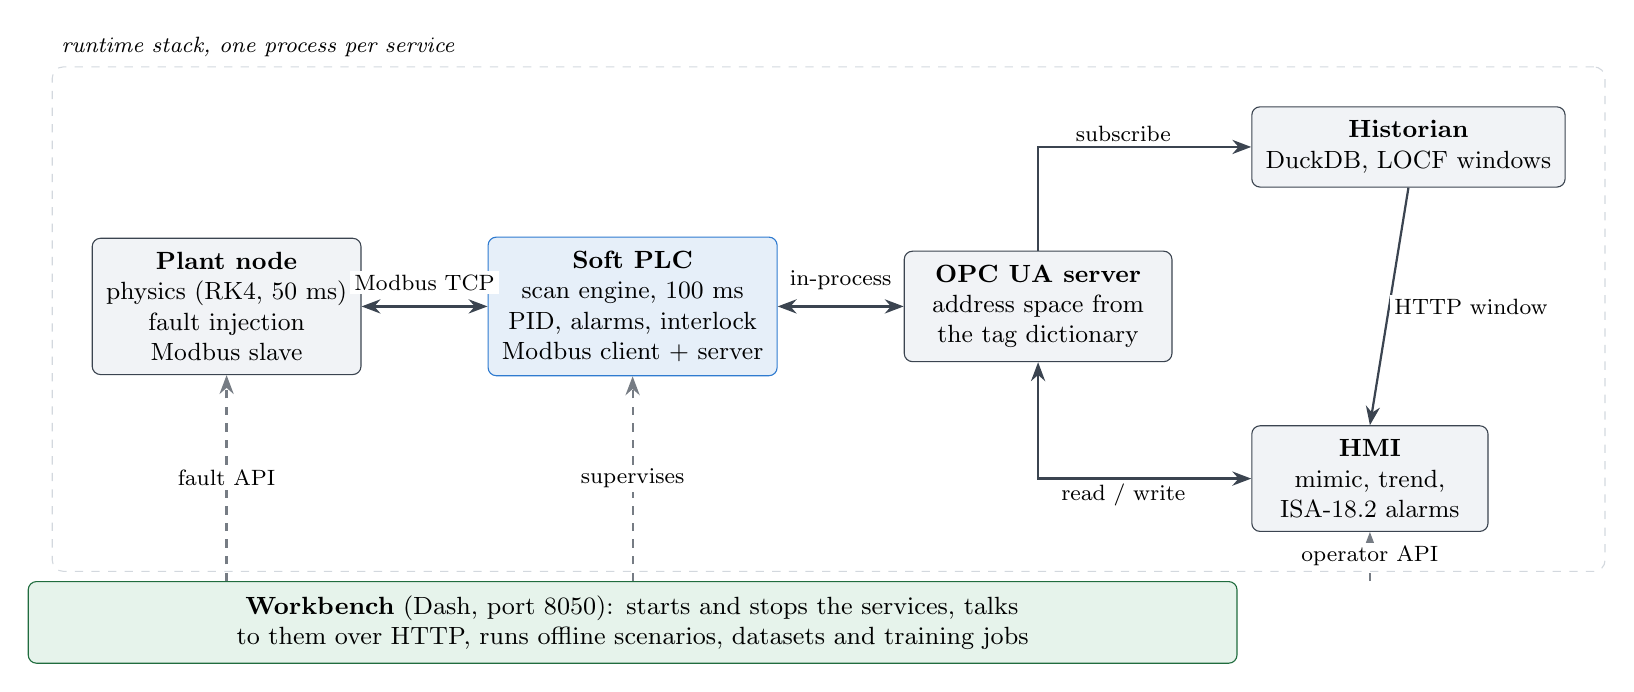
\begin{tikzpicture}[node distance=9mm and 16mm]
  \node[box,minimum width=34mm] (plant) {\textbf{Plant node}\\physics (RK4, 50 ms)\\fault injection\\Modbus slave};
  \node[hot,minimum width=34mm,right=of plant] (plc) {\textbf{Soft PLC}\\scan engine, 100 ms\\PID, alarms, interlock\\Modbus client + server};
  \node[box,minimum width=34mm,right=of plc] (opc) {\textbf{OPC UA server}\\address space from\\the tag dictionary};
  \node[box,minimum width=30mm,above right=8mm and 10mm of opc] (hist) {\textbf{Historian}\\DuckDB, LOCF windows};
  \node[box,minimum width=30mm,below right=8mm and 10mm of opc] (hmi) {\textbf{HMI}\\mimic, trend,\\ISA-18.2 alarms};
  \draw[flow,<->] (plant) -- node[lbl,above=4pt]{Modbus TCP} (plc);
  \draw[flow,<->] (plc) -- node[lbl,above=4pt]{in-process} (opc);
  \draw[flow] (opc) |- node[lbl,pos=0.7,above]{subscribe} (hist);
  \draw[flow,<->] (opc) |- node[lbl,pos=0.7,below]{read / write} (hmi);
  \draw[flow] (hist.south) -- node[lbl,right]{HTTP window} (hmi.north);
  \node[good,text width=150mm,below=26mm of plc] (wb) {\textbf{Workbench} (Dash, port 8050): starts and stops the services,
  talks to them over HTTP, runs offline scenarios, datasets and training jobs};
  \draw[dflow] (wb.north -| plant) -- node[lbl]{fault API} (plant.south);
  \draw[dflow] (wb.north -| plc) -- node[lbl]{supervises} (plc.south);
  \draw[dflow] (wb.north -| hmi) -- node[lbl]{operator API} (hmi.south);
  \begin{scope}[on background layer]
    \node[draw=linegrey,dashed,rounded corners,fit=(plant)(plc)(opc)(hist)(hmi),inner sep=5mm,
      label={[font=\footnotesize\itshape,anchor=south west]north west:runtime stack, one process per service}] {};
  \end{scope}
\end{tikzpicture}}
\caption{Runtime architecture. Each box in the dashed frame is a separate
operating-system process. The workbench is a client of the stack, never a
participant in it.}
\label{fig:arch}
\end{figure}

Three design rules recur throughout the code base and this manual:

\begin{enumerate}
  \item \textbf{One source of truth per fact.} Every signal is declared once,
        in the tag dictionary \code{pyplant/tags.py}. Addresses, scale factors,
        alarm limits and OPC UA paths are derived from it, never retyped.
  \item \textbf{Ownership.} Every tag has exactly one owner process. A process
        writes only what it owns. The plant cannot write controller outputs and
        the HMI cannot write measurements.
  \item \textbf{The same code drives the live plant and the datasets.} The
        offline scenario runner and the live plant node step the identical
        \code{Simulation} object with the identical PLC \code{Program}, so the
        training data cannot drift away from the running plant.
\end{enumerate}

\section{The two execution paths}

\begin{figure}[htbp]
\centering
\scalebox{0.8}{%
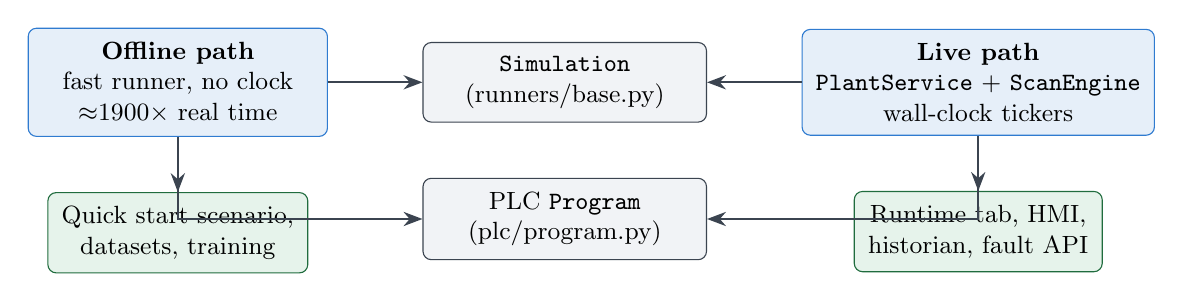
\begin{tikzpicture}[node distance=7mm and 10mm]
  \node[box,minimum width=36mm] (sim) {\code{Simulation}\\(runners/base.py)};
  \node[box,minimum width=36mm,below=of sim] (prog) {PLC \code{Program}\\(plc/program.py)};
  \node[hot,left=12mm of sim,minimum width=38mm] (fast) {\textbf{Offline path}\\fast runner, no clock\\$\approx$1900$\times$ real time};
  \node[hot,right=12mm of sim,minimum width=38mm] (live) {\textbf{Live path}\\\code{PlantService} + \code{ScanEngine}\\wall-clock tickers};
  \node[good,below=of fast] (ds) {Quick start scenario,\\datasets, training};
  \node[good,below=of live] (rt) {Runtime tab, HMI,\\historian, fault API};
  \draw[flow] (fast) -- (sim); \draw[flow] (live) -- (sim);
  \draw[flow] (fast) |- (prog); \draw[flow] (live) |- (prog);
  \draw[flow] (fast) -- (ds); \draw[flow] (live) -- (rt);
\end{tikzpicture}}
\caption{Two drivers, one model. Neither path owns the physics or the logic.}
\label{fig:paths}
\end{figure}

The \emph{offline path} (Figure~\ref{fig:paths}, left) runs the plant and the
PLC program in a tight loop with no clock and no network. A simulated hour
takes under two seconds. It is used by the Quick start tab, by dataset
generation and by the tests. The \emph{live path} (right) runs the same objects
against wall-clock schedulers, splits them into processes and connects them
with Modbus and OPC UA. It is used whenever the stack is started.

\section{Conventions in this manual}

\begin{itemize}
  \item Tag names are set in sans serif, e.g.\ \tg{LT101}.
  \item File names, Python identifiers and commands are set in
        typewriter type, e.g.\ \code{pyplant/plc/pid.py}.
  \item Buttons and labels in the workbench are set in bold, e.g.\
        \ui{Start stack}.
  \item Physical quantities inside the code are SI. Engineering units
        (mm, L/min, kPa, \%) appear only at the instrument boundary.
\end{itemize}

\chapter{Installation and first run}
\label{ch:install}

\section{Requirements}

\begin{center}
\begin{tabularx}{\textwidth}{@{}lX@{}}
\toprule
Item & Requirement \\
\midrule
Python & 3.11 or newer (3.12 is used for development) \\
Operating system & Windows, Linux or macOS \\
Memory & 2\,GB free is ample \\
Runtime libraries & numpy, pandas, pymodbus 3.8.x, asyncua, duckdb, fastapi, uvicorn, httpx \\
Machine learning (\code{ml} extra) & scikit-learn, pyarrow, joblib \\
Workbench UI (\code{ui} extra) & dash, plotly \\
Tests (\code{dev} extra) & pytest \\
\bottomrule
\end{tabularx}
\end{center}

\begin{warn}[pymodbus must stay on 3.8.x]
The 3.15 line of pymodbus replaced the datastore API this project uses and no
longer offers a way to update served values from outside the server, which is
what a live plant does twenty times a second. \code{pyproject.toml} pins
\code{pymodbus>=3.8,<3.9}; do not relax it.
\end{warn}

\section{Installing}

From the directory that contains \code{pyproject.toml}:

\begin{lstlisting}[style=sh]
# a dedicated environment is recommended
conda create -n pyplant python=3.12 -y
conda activate pyplant

pip uninstall -y pyplant          # an unrelated PyPI package has this name
pip install -e ".[ml,ui,dev]"     # everything: stack, ML, workbench, tests
python -c "import pyplant.hist.db; print('ok')"
\end{lstlisting}

The \code{-e} (editable) flag puts this directory on the Python path, so an
edited file takes effect without reinstalling and \code{python -m pyplant...}
works from any directory.

\begin{note}[Windows with several Pythons]
If \code{python --version} reports something older than 3.11, call the
environment's interpreter explicitly, for example
\begin{lstlisting}[style=sh]
C:\Users\you\anaconda3\envs\pyplant\python.exe -m pyplant.workbench.app
\end{lstlisting}
\end{note}

\section{Checking the installation}

\begin{lstlisting}[style=sh]
python -m pyplant.tags          # prints the tag list and the Modbus block plan
pytest -q                       # full suite, about five minutes
pytest -q -m "not slow"         # skips tests that start real subprocesses
\end{lstlisting}

\section{Starting the workbench}

\begin{lstlisting}[style=sh]
python -m pyplant.workbench.app --workspace ./work/demo --base-port 5400
\end{lstlisting}

Then open \url{http://127.0.0.1:8050}. The options are:

\begin{center}
\begin{tabular}{@{}lll@{}}
\toprule
Option & Default & Meaning \\
\midrule
\code{--workspace} & \code{./work/demo} & directory holding config, data, models and logs \\
\code{--base-port} & 5400 & first of six consecutive ports for the stack \\
\code{--host} & 127.0.0.1 & interface the workbench page listens on \\
\code{--port} & 8050 & port of the workbench page \\
\code{--debug} & off & Dash debug mode with hot reload \\
\bottomrule
\end{tabular}
\end{center}

With \code{--base-port 5400} the stack uses the ports in
Table~\ref{tab:ports}. Several people on one machine can each run a stack by
choosing different base ports.

\begin{table}[htbp]
\centering
\begin{tabular}{@{}llll@{}}
\toprule
Port & Offset & Service & Protocol \\
\midrule
5400 & +0 & plant Modbus slave & Modbus TCP \\
5401 & +1 & plant fault-injection API & HTTP \\
5402 & +2 & PLC Modbus server (SCADA side) & Modbus TCP \\
5403 & +3 & PLC OPC UA endpoint, \code{/pyplant/} & OPC UA \\
5404 & +4 & historian query API & HTTP \\
5405 & +5 & HMI operator page and API & HTTP \\
\bottomrule
\end{tabular}
\caption{Ports allocated from the base port.}
\label{tab:ports}
\end{table}

\section{The workspace directory}

Everything a session produces lives in the workspace, and nothing it produces
lives anywhere else:

\begin{lstlisting}[style=sh]
work/demo/
  config.json          speed, dt, ports, plant, loop and data settings
  runs.jsonl           append-only log of every action and its result
  dataset.parquet      the generated, labelled dataset
  history.duckdb       the historian database of the live stack
  artifacts/           trained detectors, manifest.json, metrics.json, per-run CSVs
  jobs/                progress files of background jobs and service logs
\end{lstlisting}

Deleting the workspace is always safe: the next start recreates it with
default settings.

\section{Running the stack by hand}

The workbench starts the four services for you, but each can be started from
a terminal. This is useful for debugging and is exactly what the workbench
runs (the Runtime tab shows the command lines).

\begin{lstlisting}[style=sh]
python -m pyplant.services.plant     --port 5020 --control-port 5021
python -m pyplant.services.plc       --plant-port 5020 --port 5022 --opcua-port 5023
python -m pyplant.services.historian --endpoint opc.tcp://127.0.0.1:5023/pyplant/ \
                                     --db history.duckdb --api-port 5024
python -m pyplant.services.hmi       --endpoint opc.tcp://127.0.0.1:5023/pyplant/ \
                                     --history http://127.0.0.1:5024 --port 5025
\end{lstlisting}

Start them in this order; each depends on the one before it. All command-line
options are listed in Section~\ref{sec:cli}.

\chapter{The workbench}
\label{ch:workbench}

The workbench is the single web page from which the whole toolbox is driven.
It holds no process state of its own: every value on the screen was read from
the HMI, the plant's fault API or the historian a moment ago. Long jobs
(dataset generation, training) run in separate processes and report progress
through files, so the page never blocks.

\section{Layout}

\begin{figure}[htbp]
\centering
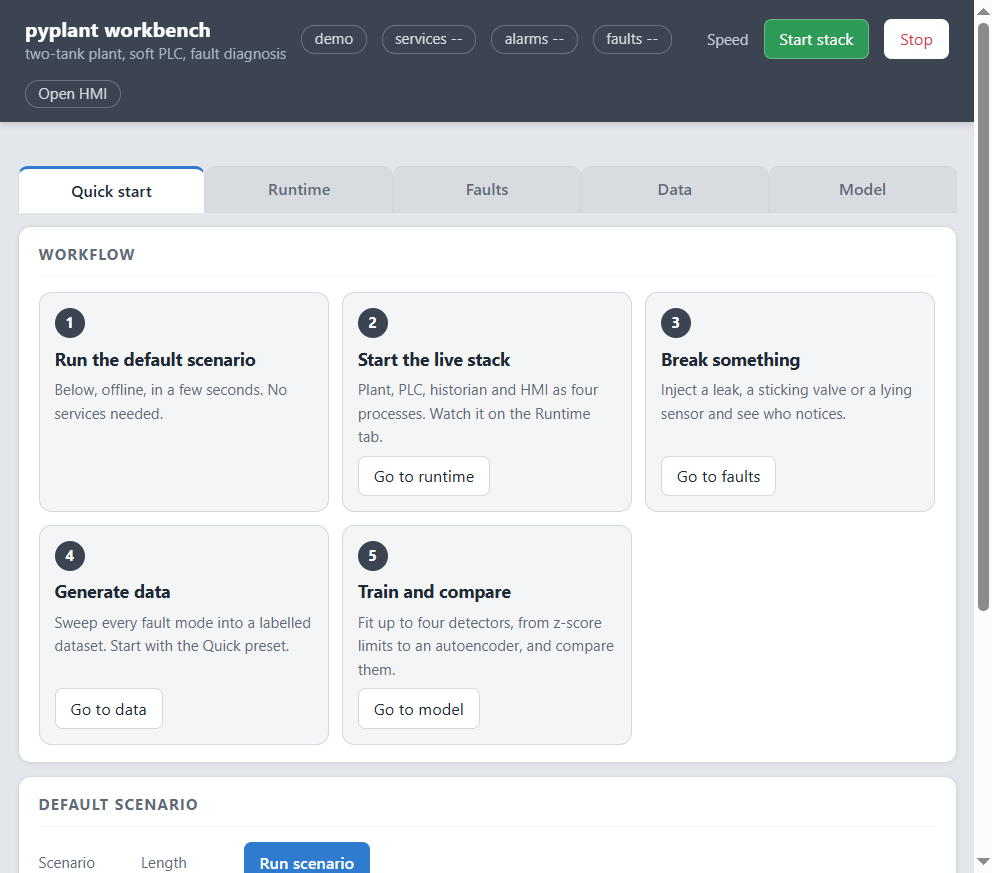
\includegraphics[width=0.6\textwidth]{quickstart_workflow.png}
\caption{The workbench header and the Quick start tab with its five workflow
cards.}
\label{fig:wb-header}
\end{figure}

\subsection*{Header}
The dark grey header stays at the top of the page and contains:
\begin{itemize}
  \item the workspace name;
  \item three status pills: services up (e.g.\ \ui{4/4 services}),
        unacknowledged alarms, and active faults. Green means healthy, amber
        partial, red attention;
  \item the \ui{Speed} selector, a real-time factor applied when the stack
        starts (Section~\ref{sec:speed});
  \item \ui{Start stack} and \ui{Stop}, which launch or terminate the four
        services in dependency order;
  \item \ui{Open HMI}, a link to the stand-alone operator page.
\end{itemize}

\subsection*{Tabs}
Below the header are five tabs. All of them are present in the page at all
times and merely hidden, so switching is instant and no callback ever fires
against a missing component.

\begin{center}
\begin{tabularx}{\textwidth}{@{}lX@{}}
\toprule
Tab & Purpose \\
\midrule
\ui{Quick start} & the opening page: workflow cards, the default scenario run offline, and a one-click live demo \\
\ui{Runtime} & service status, live mimic diagram, LIC101 faceplate and operator commands, trend, alarm list \\
\ui{Faults} & one-click fault presets, a custom fault builder, the active-fault list, ground truth against instrument readings \\
\ui{Data} & generation of the labelled scenario dataset, with presets and progress \\
\ui{Model} & selection and training of detection methods, comparison table, per-fault-mode results \\
\bottomrule
\end{tabularx}
\end{center}

\section{Quick start tab}

\subsection{Workflow cards}
Five numbered cards describe the recommended order of work. A card turns
green when its step is done, judged from what the workspace actually holds:

\begin{enumerate}
  \item \ui{Run the default scenario} --- done once a scenario has run in this session;
  \item \ui{Start the live stack} --- done while the HMI answers;
  \item \ui{Break something} --- done once any fault has been injected;
  \item \ui{Generate data} --- done once \code{dataset.parquet} exists;
  \item \ui{Train and compare} --- done once \code{artifacts/metrics.json} exists.
\end{enumerate}
Each card from step 2 on has a \ui{Go to ...} button that opens the right tab.

\subsection{Default scenario}

\begin{figure}[htbp]
\centering
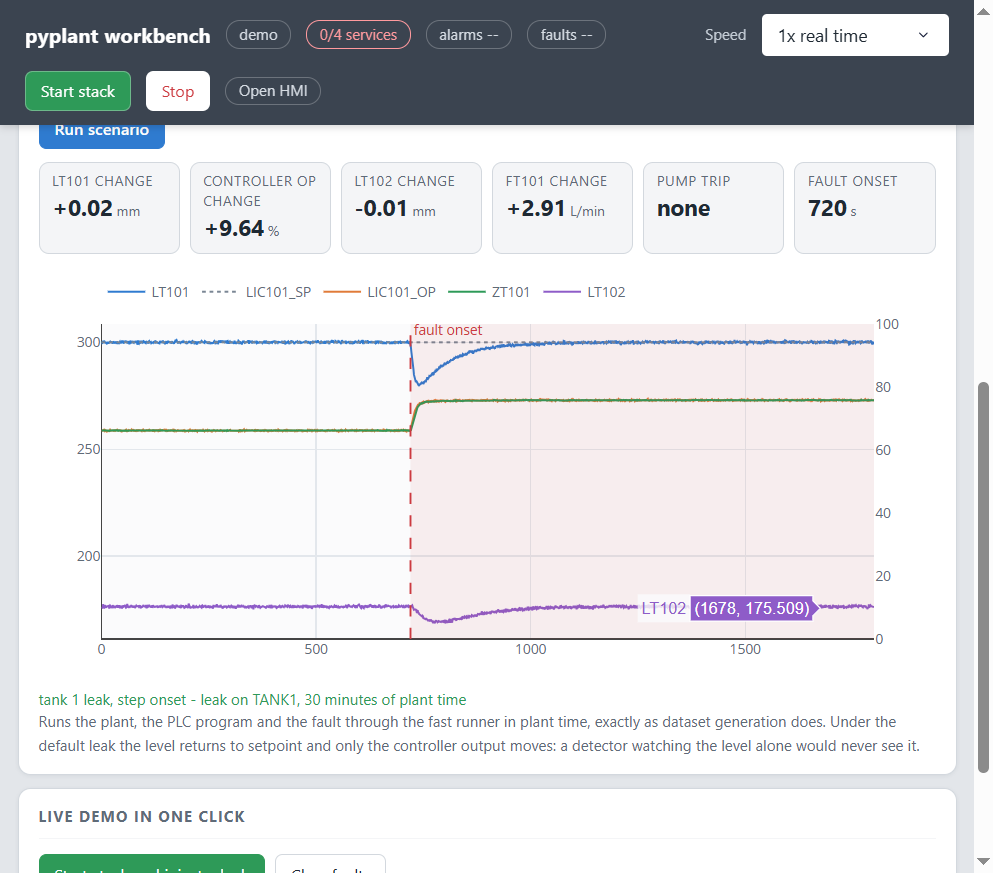
\includegraphics[width=0.6\textwidth]{quickstart_scenario.png}
\caption{The default scenario: an abrupt leak in tank 1 at $t = 720$\,s. The
level (blue) dips and returns to the setpoint (dotted); the controller output
(orange) and the valve position (green) rise by about 10\%. The summary cards
quantify the change.}
\label{fig:qs-scenario}
\end{figure}

When the page opens it immediately runs the default scenario, an abrupt leak
in tank~1, through the offline runner. No services are needed and the run
takes a few seconds. The controls are:

\begin{description}
  \item[Scenario] any of the nine library scenarios: normal operation, abrupt
        leak (default), slow leak, pump wear, fouling, valve stiction, sensor
        bias, sensor drift, frozen sensor.
  \item[Length] 15, 30 or 60 minutes of plant time. The fault starts at 40\%
        of the length.
  \item[setpoint moves] off by default, so the setpoint is held at 300\,mm and
        everything that moves is caused by the fault. Ticking it adds the
        standard setpoint programme (300, 340, 280, 300\,mm at 0, 15, 30 and
        45 minutes).
  \item[Run scenario] reruns with the chosen settings.
\end{description}

The summary cards compare the last five minutes before onset with the last
five minutes of the run: change in \tg{LT101}, controller output, \tg{LT102}
and \tg{FT101}, the time of any pump trip, and the onset time. The chart has
levels on the left axis and percentages on the right; the faulty period is
shaded red.

\subsection{Live demo in one click}
\ui{Start stack and inject a leak} starts the four services if they are not
already running, waits until each answers, and injects a
$5\times10^{-5}$\,m$^2$ leak into the live plant. Open the Runtime tab to
watch the controller output climb while the level holds. \ui{Clear faults}
removes every injected fault and leaves the instrument noise in place.

\section{Runtime tab}

\begin{description}
  \item[Services] one row per service with state, process id, port and role,
        and the exact command line the supervisor ran.
  \item[Unit 1] the mimic: pump, valve filled to its measured stem position,
        both tanks filled to their levels, flows and pump pressure. Pipes turn
        blue when they carry flow. A red frame marks a level alarm and a red
        banner a tripped interlock. Below it, cards for \tg{FT101},
        \tg{FT102}, \tg{PT101}, \tg{ZT101}, scan time and overrun count.
  \item[LIC101] the controller faceplate: PV, SP, OP, error, mode and pump
        state, plus the operator commands:
        \begin{itemize}
          \item \ui{Setpoint} + \ui{Write} --- 0 to 600\,mm. Values outside
                the span are rejected with a visible error, never clamped.
          \item \ui{Manual OP} + \ui{Write} --- valve demand in manual mode, 0 to 100\%.
          \item \ui{Auto} / \ui{Manual} --- controller mode (bumpless both ways).
          \item \ui{Start} / \ui{Stop} --- pump request.
          \item \ui{Reset interlock} --- pulses the reset bit. A latched trip
                clears only if its cause has gone.
        \end{itemize}
  \item[Trend] \tg{LT101}, \tg{LIC101_SP} and \tg{LT102} in mm on the left
        axis and \tg{LIC101_OP} in \% on the right, over 2, 5, 15 or 60
        minutes, read from the historian.
  \item[Alarms] the ISA-18.2 alarm list with priority, tag, message, state,
        time in and count, and per-row \ui{Ack} and \ui{Shelve} (30 minutes).
        \ui{Acknowledge all} acknowledges every alarm.
\end{description}

\section{Faults tab}

\begin{description}
  \item[Break something] seven presets, one click each: leak in tank 1, slow
        leak (15 minute ramp), sticking valve, worn pump, fouled interconnect,
        LT101 reading 25\,mm high, LT101 frozen. Some print a suggested next
        step; for instance a frozen transmitter on setpoint gives the
        controller nothing to act on until you move the setpoint.
  \item[Or build one] any fault kind with its own magnitude (units shown
        beside the field), sensor tag for sensor faults, and ramp time.
        Default magnitudes are filled in when the kind changes.
  \item[Active faults] id, kind, target, state, magnitude, start and ramp.
  \item[Ground truth] what each instrument reads against what the plant
        really is. Under a sensor fault the two disagree; under a process
        fault they agree and the fault appears in the controller output.
\end{description}

\begin{note}[Injection is separate from the control system]
Faults are injected through the plant's own API, not through the PLC or the
HMI. Neither the operator page nor a detector is told that a fault exists;
the only way to know is to observe the plant. This keeps the diagnosis problem
honest.
\end{note}

\section{Data tab}

\begin{description}
  \item[Preset] fills the four fields below:
  \begin{center}
  \begin{tabular}{@{}lrrrrr@{}}
  \toprule
  Preset & Run length & Magnitudes & Repeats & Normal runs & Typical time \\
  \midrule
  Quick & 1200\,s & 1 & 1 & 6 & about 1.5 min \\
  Standard & 3600\,s & 3 & 2 & 10 & about 4 min \\
  Thorough & 3600\,s & 5 & 3 & 16 & about 10 min \\
  \bottomrule
  \end{tabular}
  \end{center}
  \item[Run length] seconds of recorded plant time per run.
  \item[Magnitudes] how many fault sizes per mode, spread from 0.5 to 1.5
        times the library value.
  \item[Repeats] runs per mode and magnitude, each with its own seed and a
        random onset between 25\% and 60\% of the run.
  \item[Normal runs] fault-free runs. At least three are needed (train,
        calibrate, test); more give a better false-alarm estimate.
  \item[Generate / Cancel] start or stop the background job. The progress bar
        and \ui{Recent runs} table update every three seconds.
\end{description}

\section{Model tab}

\begin{figure}[htbp]
\centering
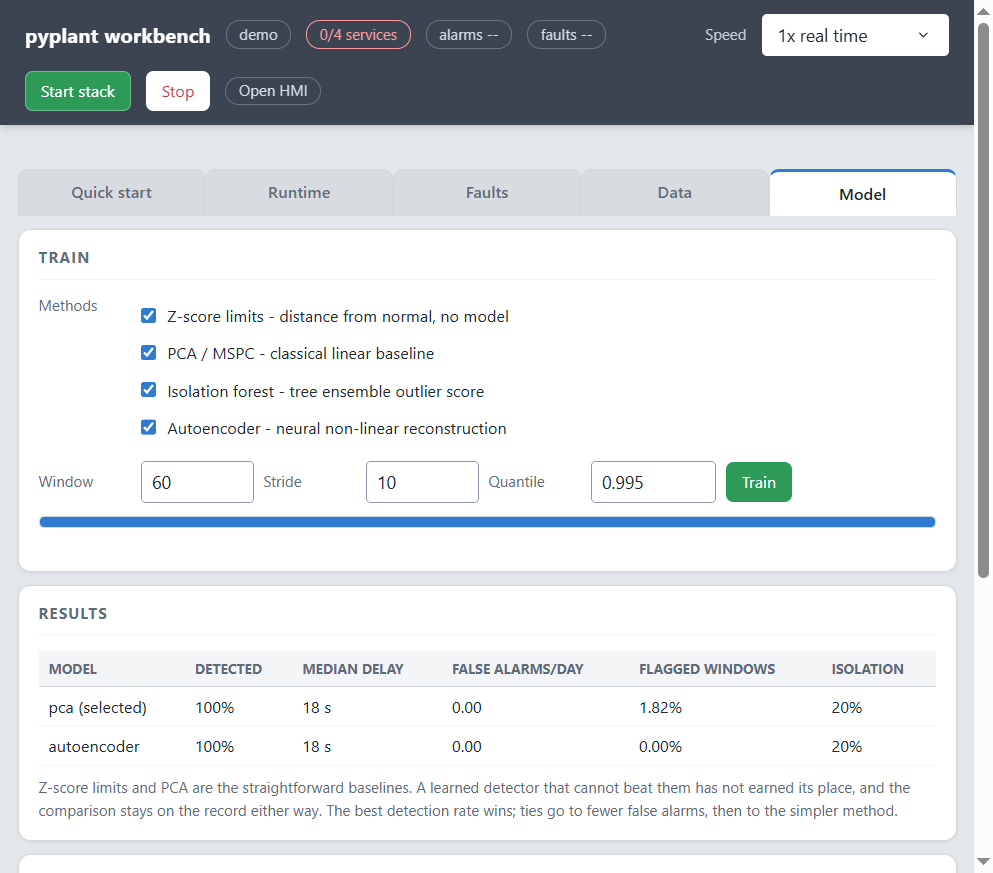
\includegraphics[width=0.6\textwidth]{model_tab.png}
\caption{The Model tab: method selection, window settings and the comparison
table.}
\label{fig:model-tab}
\end{figure}

\begin{description}
  \item[Methods] tick any of the four detectors (Chapter~\ref{ch:ml} and
        \ref{ch:dl}): z-score limits, PCA/MSPC, isolation forest, autoencoder.
  \item[Window] samples per window (1\,Hz, so 60 is one minute).
  \item[Stride] samples between consecutive windows.
  \item[Quantile] the fraction of held-out normal windows that must lie below
        the alarm threshold, e.g.\ 0.995.
  \item[Train] fits every ticked method, evaluates it and deploys the best.
  \item[Results] detection rate, median detection delay, false alarms per
        day, flagged-window rate and isolation accuracy per method.
  \item[By fault mode] for the selected method: runs, detection rate, median
        delay, the channel that contributed most, and the channel physics
        expects.
\end{description}

\section{Speed}
\label{sec:speed}

Speed is a real-time factor applied to both the plant and the PLC tickers:
at $4\times$ a 100\,ms scan runs every 25\,ms of wall time. Slow faults need
it: a stiction limit cycle takes several process time constants to establish,
and this plant's time constant is 72\,s.

\begin{warn}[Windows timer granularity]
Windows schedules sleeps in steps of about 15.6\,ms. Above $4\times$ the scan
period falls below that, every scan lands late and \tg{SCAN_OVERRUNS} climbs.
The controller still works; the diagnostics are telling the truth. Keep speed
at 4 or below on Windows. Linux and macOS manage $20\times$.
\end{warn}

\chapter{Walkthrough: one leak, from step 0 to a trained detector}
\label{ch:walkthrough}

This chapter follows a single, fixed scenario through every part of the
workbench. Every figure is a real screenshot taken while writing this manual,
in the order the steps happen, and each one is followed by a table that names
the elements on screen and says what they do. Section~\ref{sec:wt-numbers}
collects the numbers to expect at each step.

\begin{note}[The scenario]
Unit~1 runs in automatic at a level of 300\,mm. The operator raises the
setpoint to 340\,mm. Then a hole opens in tank~1 (the \ui{Leak in tank 1}
preset, an effective leak area of $5\times10^{-5}$\,m$^2$). We watch the
controller hide the leak, then confirm it on the operator HMI. Finally we
generate a labelled dataset and train four detectors to see which one would
have caught it. Workspace \code{work/manual}, base port 5400, speed
1$\times$ real time.
\end{note}

\begin{figure}[H]
\centering
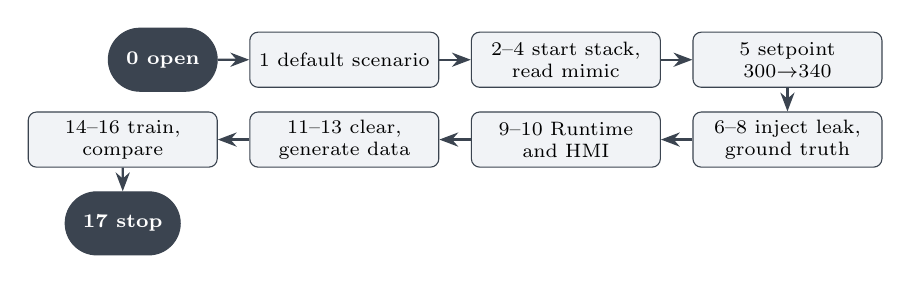
\begin{tikzpicture}[node distance=3mm and 4mm,
  st/.style={box,minimum width=24mm,minimum height=7mm,font=\scriptsize,inner sep=2pt}]
  \node[term,font=\scriptsize\bfseries] (s0) {0 open};
  \node[st,right=of s0] (s1) {1 default scenario};
  \node[st,right=of s1] (s2) {2--4 start stack,\\read mimic};
  \node[st,right=of s2] (s5) {5 setpoint\\300$\to$340};
  \node[bad,st,below=of s5] (s7) {6--8 inject leak,\\ground truth};
  \node[st,left=of s7] (s9) {9--10 Runtime\\and HMI};
  \node[st,left=of s9] (s11) {11--13 clear,\\generate data};
  \node[good,st,left=of s11] (s14) {14--16 train,\\compare};
  \node[term,font=\scriptsize\bfseries,below=of s14] (s17) {17 stop};
  \draw[flow] (s0) -- (s1);
  \draw[flow] (s1) -- (s2);
  \draw[flow] (s2) -- (s5);
  \draw[flow] (s5) -- (s7);
  \draw[flow] (s7) -- (s9);
  \draw[flow] (s9) -- (s11);
  \draw[flow] (s11) -- (s14);
  \draw[flow] (s14) -- (s17);
\end{tikzpicture}
\caption{The eighteen steps of the walkthrough.}
\label{fig:wt-map}
\end{figure}

% ---------------------------------------------------------------------------
\section{Step 0: open the workbench}

Start the workbench on its own workspace so the walkthrough does not disturb
other work:
\begin{lstlisting}[style=sh]
conda activate pyplant
python -m pyplant.workbench.app --workspace ./work/manual
\end{lstlisting}
Open \url{http://127.0.0.1:8050}. The Quick start tab opens first
(Figure~\ref{fig:s00_open}).

\shot{s00_open}{Step 0: the workbench as it opens, with nothing running.}

\begin{elements}
pyplant workbench & Title. The dark header stays on screen on every tab. \\
manual (badge) & Name of the workspace folder. Every file the session
  writes goes there. \\
0/4 services (badge) & How many of the four services (plant, PLC, historian,
  HMI) are up. It is red below 4/4 and green at 4/4. \\
alarms -- / faults -- & Live alarm and fault counts. They show ``--'' while
  the stack is down, because nobody is there to ask. \\
Speed & Plant-time multiplier for the live stack (1$\times$ to
  20$\times$). It takes effect at the next \ui{Start stack}; see
  Section~\ref{sec:speed}. \\
Start stack & Green button. Launches the four services as separate
  processes. \\
Stop & Stops every service the workbench started. \\
Open HMI & Link that opens the operator page on port 5405 in a new tab. \\
Tabs & \ui{Quick start}, \ui{Runtime}, \ui{Faults}, \ui{Data},
  \ui{Model}. The active tab is white with a blue top edge. \\
Workflow cards 1--5 & The recommended order of work. Card~1 is highlighted
  green because it needs no services. The \ui{Go to \ldots} buttons switch
  tabs. \\
\end{elements}

% ---------------------------------------------------------------------------
\section{Step 1: run the default scenario offline}

Scroll down to \ui{Default scenario}. Leave \ui{Scenario} on
\ui{Leak in tank 1 (default)}, \ui{Length} on \ui{30 minutes}, and
\ui{setpoint moves} unticked, then press \ui{Run scenario}. The fast runner
simulates 30 minutes of plant time in a few seconds, without any service.

\shot{s01_scenario}{Step 1: the default scenario result.}

\begin{elements}
Scenario (dropdown) & Which built-in scenario to run. The default is the
  tank-1 leak. \\
Length (dropdown) & Plant time to simulate. \\
setpoint moves & When ticked, the scenario also steps the setpoint, so the
  fault has to be told apart from normal operation. \\
Run scenario & Blue button. Runs the scenario and redraws everything
  below it. \\
LT101 CHANGE & End level minus start level: \textbf{+0.02\,mm}. The loop
  holds the level, so the leak is \emph{invisible} in the level. \\
CONTROLLER OP CHANGE & \textbf{+9.64\,\%}. The controller opens the valve to
  feed the leak. This is where the fault actually shows. \\
LT102 / FT101 CHANGE & Tank~2 is unaffected (\textbf{$-$0.01\,mm}); the
  inflow rises by \textbf{2.91\,L/min}, which equals the leak flow. \\
PUMP TRIP & Whether the low-level interlock tripped (\textbf{none}). \\
FAULT ONSET & Plant time at which the leak opened (\textbf{720\,s}). \\
Chart & Left axis: levels (\tg{LT101} blue, \tg{LT102} purple, setpoint
  grey dashes). Right axis: \tg{LIC101_OP} orange and \tg{ZT101} green
  (\%). The red band marks the fault. \\
Caption line & Green text naming the scenario and length that produced the
  chart. \\
\end{elements}

The chart is the whole lesson of the chapter in one picture. At onset the
level dips about 20\,mm and recovers within a few minutes. The valve then
stays about 10 points more open for as long as the leak lasts.

% ---------------------------------------------------------------------------
\section{Step 2: look at the Runtime tab before starting}

Click the \ui{Runtime} tab. With nothing running, every service is down
and the mimic shows dashes (Figure~\ref{fig:s02_runtime_stopped}).

\shot{s02_runtime_stopped}{Step 2: the Runtime tab with the stack down.}

\begin{elements}
SERVICES table & One row per service: name, \ui{STATE} pill (red
  \ui{down} / green \ui{up}), operating-system \ui{PID}, \ui{PORT} and
  \ui{ROLE}. \\
Hint line & ``Not running. Start the stack to see live values.'' \\
UNIT 1 mimic & The process drawing. Values are ``--'' until the PLC
  answers. \\
\end{elements}

% ---------------------------------------------------------------------------
\section{Step 3: start the stack}

Keep \ui{Speed} at \ui{1x real time} and press \ui{Start stack}. After a
few seconds the badge turns green at \ui{4/4 services}, and the alarm and
fault counts change from ``--'' to 0.

\shot{s03_runtime_services}{Step 3: all four services up.}

\begin{elements}
stack started at 1x & Green confirmation under the header. \\
STATE = up & Each process answered its health check. \\
PID & Process id; useful if you need to look at a service in Task
  Manager. \\
PORT & plant 5400 (Modbus), plc 5402 (Modbus server; OPC UA on 5403),
  historian 5404, hmi 5405. \\
Command line (grey text) & The exact command the supervisor ran for the
  last service listed. Copy it to run that service by hand. \\
\end{elements}

% ---------------------------------------------------------------------------
\section{Step 4: read the mimic}

Scroll to \ui{UNIT 1}. This is the healthy reference picture; keep it in
mind for step~9.

\shot{s04_runtime_mimic}{Step 4: the healthy plant at steady state.}

\begin{elements}
PMP101 & Pump symbol. A green ring means running. \\
FCV101 66.1\% & Control valve. The fill of the small box is the stem
  position. \\
PT101 / FT101 labels & Pump discharge pressure (50.3\,kPa) and inflow
  (10.08\,L/min), drawn on the pipe. \\
TANK 1 / TANK 2 & Live levels \tg{LT101} = 300.0\,mm and \tg{LT102} =
  176.8\,mm. The blue fill is to scale. \\
drain 10.05 L/min & Outflow of tank~2 (\tg{FT102}). In steady state it
  equals \tg{FT101}. \\
Tiles FT101 \ldots ZT101 & The same measurements as numbers. \\
SCAN / OVERRUNS & PLC scan time (3.70\,ms of a 100\,ms budget) and the count
  of scans that ran over. A non-zero OVERRUNS means the PC is too slow for
  the chosen speed. \\
\end{elements}

% ---------------------------------------------------------------------------
\section{Step 5: operate LIC101, a setpoint step}

On the \ui{LIC101} faceplate, type \code{340} in \ui{Setpoint} and press its
\ui{Write} button. Watch the trend for about two minutes.

\shot{s05_faceplate_trend}{Step 5: the faceplate after the setpoint step to 340\,mm, with the trend.}

\begin{elements}
PV / SP / OP / ERROR & Process value 339.7\,mm, setpoint 340.0\,mm,
  controller output 68.6\,\%, error 0.3\,mm. \\
MODE / PUMP & AUTO (the PID drives the valve) and RUN. \\
Setpoint + Write & Sends a new setpoint to the PLC. ``sp-write accepted''
  confirms it. \\
Manual OP + Write & Valve opening to use in Manual mode. Ignored in Auto. \\
Auto / Manual & Switches the controller mode. The PLC changes mode
  bumplessly. \\
Pump Start / Stop & Operator commands to PMP101. \\
Reset interlock & Clears a latched low-level trip once the level has
  recovered. \\
TREND, Window & Historian trend, 5 minutes by default. Levels on the left
  axis, OP on the right axis. \\
\end{elements}

The step response is clean. The output kicks up to about 80\,\%, the level
rises to 340\,mm in roughly a minute without overshoot, and the output
settles at 68.6\,\%, a little higher than before because a fuller tank~1
drains faster.

% ---------------------------------------------------------------------------
\section{Step 6: open the Faults tab}

Click the \ui{Faults} tab. Before anything is injected, \ui{Active faults}
reads ``Plant is healthy.''

\shot{s06_faults_empty}{Step 6: the Faults tab, nothing injected.}

\begin{elements}
BREAK SOMETHING & One-click presets (red outline). Each injects a fault of
  a sensible size: \ui{Leak in tank 1}, \ui{Slow leak (15 min ramp)},
  \ui{Sticking valve}, \ui{Worn pump}, \ui{Fouled interconnect},
  \ui{LT101 reads 25 mm high}, \ui{LT101 frozen}. \\
Clear all faults & Removes every active fault at once. \\
OR BUILD ONE: Kind & Fault type, alphabetical: \code{fouling}, \code{leak},
  \code{pump_wear}, \code{sensor_bias}, \code{sensor_drift},
  \code{sensor_noise}, \code{sensor_stuck}, \code{stiction}. \\
Magnitude ($-$/$+$) & Size of the fault. The text on the right gives its
  unit for the chosen kind (here m$^2$ of effective leak area). \\
Sensor & Which transmitter a sensor fault acts on. It is greyed out for
  process faults. \\
Ramp (s) & 0 for a step; otherwise the time the fault takes to grow to
  full size. \\
Inject & Applies the custom fault. \\
Grey note & Injection is separate from control: neither the HMI nor a
  model is told about the fault. \\
\end{elements}

% ---------------------------------------------------------------------------
\section{Step 7: inject the leak}

Press \ui{Leak in tank 1}. The message under the presets confirms the
injection and the header badge turns red at \ui{faults 1}.

\shot{s07_fault_injected}{Step 7: the leak is injected.}

\begin{elements}
faults 1 (red badge) & One fault is active in the plant. \\
Message & ``injected leak\_168 on TANK1 -- watch the Runtime tab''. The
  number is the plant time of injection, used as the fault id. \\
ACTIVE FAULTS row & \ui{ID} leak\_168, \ui{KIND} leak, \ui{TARGET} TANK1,
  \ui{STATE} active, \ui{MAGNITUDE} 0.000050, \ui{START (S)} 169,
  \ui{RAMP (S)} 0. \\
\end{elements}

% ---------------------------------------------------------------------------
\section{Step 8: check the ground truth}

Scroll down. The ground-truth table compares the plant's true state with
what each transmitter reports.

\shot{s08_truth}{Step 8: active fault and ground truth, about 30\,s after injection.}

\begin{elements}
TAG & The five measured channels. \\
TRUE & The physical value inside the simulator. \\
REPORTED & What the transmitter sends to the PLC, including noise and any
  sensor fault. \\
DIFFERENCE & Reported minus true. Here every difference is within the noise
  (below 0.3), which tells you the fault is in the \emph{process}, not in a
  sensor. Under \ui{LT101 reads 25 mm high} the LT101 row would show about
  +25. \\
\end{elements}

Notice the true level, 299.3\,mm: the leak has already pulled tank~1 about
40\,mm below the 340\,mm setpoint.

% ---------------------------------------------------------------------------
\section{Step 9: watch the controller compensate}

Go back to \ui{Runtime} and scroll to \ui{LIC101}, about two minutes after
the injection.

\shot{s09_runtime_leak}{Step 9: the loop fighting the leak. The trend shows the setpoint step from step~5, then the leak.}

\begin{elements}
PV 324.6 mm, ERROR 15.4 mm & The level is still below setpoint but
  climbing back. \\
OP 93.4\,\% & The valve is almost fully open. Before the leak it was
  68.6\,\%. \\
MODE AUTO, PUMP RUN & No interlock trip; the operator sees no alarm. \\
Trend, first edge & The setpoint step from step~5 (grey) and the clean level
  response (blue). \\
Trend, second edge & The leak. The level (blue) drops to about 290\,mm while
  the output (orange) jumps to about 92\,\% and stays there. The level
  recovers slowly, because the valve has little travel left. \\
\end{elements}

This is the signature to remember: a \emph{process} fault moves the
controller output, while the level only dips and then returns.

% ---------------------------------------------------------------------------
\section{Step 10: see it as the operator, on the HMI}

Click \ui{Open HMI} in the header, or open \url{http://127.0.0.1:5405}. The
HMI is a separate service and reads everything over OPC UA.

\shot{s10_hmi}{Step 10: the operator HMI during the leak.}

\begin{elements}
pyplant -- Unit 1 & HMI header. \ui{connected} (green) means the OPC UA
  session is live. It also shows the alarm count, the controller mode badge
  \ui{AUTO}, and the PLC timestamp. \\
MIMIC & Same process picture, in a dark ISA-101 style: tank~1 328.4\,mm,
  tank~2 188.4\,mm. \\
FT101 / PT101 / ZT101 & Inflow up to 18.30\,L/min (from about 10), pump
  pressure down to 27.9\,kPa (the pump runs further out on its curve), valve
  at 93.4\,\%. \\
Scan & PLC scan time, 5.9\,ms. \\
LIC101 panel & Same faceplate as the workbench: PV, SP, OP, Error, plus
  \ui{Setpoint}/\ui{Manual OP} with \ui{Write}, \ui{Auto}/\ui{Manual} and
  pump \ui{Start}/\ui{Stop}/\ui{Reset}. \\
TREND, Window & 2\,min to 1\,hour. The legend notes that OP uses the
  0--100 right-hand scale. \\
ALARMS, Acknowledge all & Further down the page (not in the screenshot).
  It stays empty in this scenario: no limit is crossed. \\
\end{elements}

\begin{warn}[Why no alarm?]
The level never crossed the low alarm, so a conventional alarm system says
nothing. A 5$\times10^{-5}$\,m$^2$ leak loses about 8\,L/min, nearly as much
as the normal throughput, and the only evidence is a valve that is 25 points
more open. Catching this is the job of the detectors trained in steps 14--16.
\end{warn}

% ---------------------------------------------------------------------------
\section{Step 11: clear the fault and open the Data tab}

Return to the workbench. On \ui{Faults} press \ui{Clear all faults}; the
header goes back to \ui{faults 0}. Then click the \ui{Data} tab.

\shot{s11_data_form}{Step 11: the Data tab with its default settings.}

\begin{elements}
Preset: Quick / Standard / Thorough & Fill the four fields below with a
  ready-made size: about 1.5, 4 or 10 minutes of computing. \\
Run length ($-$/$+$) & Plant seconds per simulated run (default 3600). \\
Magnitudes & How many fault sizes per fault mode. \\
Repeats & How many random onsets per size. \\
Normal runs & Fault-free runs. Training uses only these. \\
Generate / Cancel & Start or stop the background job. \\
Progress bar & Grey bar under the buttons. It fills blue as runs
  finish. \\
RECENT RUNS & Job history: \ui{KIND}, \ui{STATUS}, \ui{TOOK} and a
  \ui{RESULT} summary. The ``fault'' row is the \ui{Clear all faults}
  action. \\
\end{elements}

% ---------------------------------------------------------------------------
\section{Step 12: generate a Quick dataset}

Press \ui{Quick (\textasciitilde1.5 min)}. The fields change to run length
1200, magnitudes 1, repeats 1, normal runs 6. Press \ui{Generate}.

\shot{s12_data_running}{Step 12: dataset generation in progress.}

\begin{elements}
started & Green confirmation under the bar. \\
Progress bar & About a third full: runs completed out of runs planned. \\
dataset / running / 17 s & The new job, still running, with elapsed time. \\
\end{elements}

The live stack keeps running meanwhile. Dataset runs use the offline fast
runner in a separate process and do not touch the live plant.

% ---------------------------------------------------------------------------
\section{Step 13: the dataset is ready}

\shot{s13_data_done}{Step 13: dataset finished.}

\begin{elements}
Full bar & The job has finished. \\
dataset / ok / 43 s & Status and wall time. \\
RESULT & \code{{"runs": 14, "samples": 16814, "path": ...}}: 6 normal plus
  8 faulty runs, written to \code{work/manual/dataset.parquet} (1.7\,MB). \\
\end{elements}

% ---------------------------------------------------------------------------
\section{Step 14: set up training}

Click the \ui{Model} tab.

\shot{s14_model_form}{Step 14: the Model tab before training.}

\begin{elements}
Methods (checklist) & The four detectors, from simplest to most complex:
  Z-score limits, PCA/MSPC, Isolation forest, Autoencoder. Untick any you do
  not want to train. \\
Window & Samples per feature window (60). \\
Stride & Step between windows (10). \\
Quantile & The alarm threshold is this quantile of the scores on normal
  data (0.995). Higher means fewer false alarms but later detection. \\
Train & Starts the training job. \\
RESULTS / BY FAULT MODE & Empty until the first model is trained
  (``no model trained yet''). \\
\end{elements}

% ---------------------------------------------------------------------------
\section{Step 15: train and read the results}

Keep the defaults and press \ui{Train}. The message reads
``started: zscore, pca, isolation\_forest, autoencoder''. On the Quick
dataset the job takes about 12\,s, and the bar fills when it is done.

\shot{s15_model_results}{Step 15: four detectors compared.}

\begin{elements}
model & Method name. The deployed one is marked \ui{(selected)}. \\
detected & Share of faulty test runs flagged after onset: z-score 62\,\%,
  PCA 88\,\%, isolation forest 38\,\%, autoencoder 88\,\%. \\
median delay & Time from onset to first alarm (43\,s for PCA and the
  autoencoder; more than 340\,s for the others). \\
false alarms/day & Alarms on normal test runs, scaled to a day: 0.00 for
  all four. \\
flagged windows & Share of normal windows over the threshold (0.87\,\%). \\
isolation & How often the top-scoring channel was the expected one. \\
\end{elements}

PCA and the autoencoder tie on detection and false alarms, so the rule in
the grey note picks the \emph{simpler} method: PCA is deployed to
\code{artifacts/detector.joblib}.

% ---------------------------------------------------------------------------
\section{Step 16: check the leak, fault mode by fault mode}

Scroll to \ui{BY FAULT MODE}. It shows the selected detector's results for
each fault mode.

\shot{s16_by_mode}{Step 16: per-fault-mode breakdown of the selected detector.}

\begin{elements}
fault / runs & Fault mode and how many test runs it had. \\
detected / median delay & The \textbf{leak} row: 2 runs, 100\,\%
  detected, median 139\,s after onset. \\
top channel & Channel with the largest contribution at the first alarm.
  For the leak it is \tg{FLOW_IMBALANCE}, the inflow-minus-outflow residual. \\
expected & Channel physics says should respond. The leak's matches, so the
  detector also \emph{isolates} it correctly. ``not scored'' rows are
  sensor faults, where isolation is not meaningful. \\
\end{elements}

% ---------------------------------------------------------------------------
\section{Step 17: stop the stack}

Press \ui{Stop} in the header. The badge returns to \ui{0/4 services}, the
message reads ``stack stopped'', and every service shows \ui{down}.

\shot{s17_stopped}{Step 17 (final): the stack stopped.}

\begin{elements}
stack stopped & Confirmation. \\
0/4 services, alarms --, faults -- & Nothing is running any more. \\
Mimic ``-- mm'' & No live values without the PLC. \\
\end{elements}

Everything from the session stays in \code{work/manual}: \code{config.json}
(the settings used), \code{history.duckdb} (the historian),
\code{dataset.parquet}, \code{artifacts/} (all four detectors, the deployed
\code{detector.joblib}, \code{metrics.json} and per-run CSVs), and
\code{jobs/} (job records and service logs).

% ---------------------------------------------------------------------------
\section{Numbers to expect}
\label{sec:wt-numbers}

\begin{table}[H]
\centering\small
\begin{tabularx}{\linewidth}{@{}lXl@{}}
\toprule
Step & Quantity & Observed \\
\midrule
1 & OP change for the default leak (offline) & +9.6\,\% \\
4 & Healthy steady state at SP 300 & LT101 300.0, OP 66\,\%, FT101 10.1 \\
5 & After SP step to 340 & PV 339.7, OP 68.6\,\%, no overshoot \\
9 & Two minutes into the leak & PV 324.6, OP 93.4\,\%, no alarm \\
10 & HMI during the leak & FT101 18.3\,L/min, PT101 27.9\,kPa \\
13 & Quick dataset & 14 runs, 16\,814 samples, 43\,s \\
15 & Selected detector & PCA, 88\,\% detected, 0 false alarms/day \\
16 & Leak, per mode & 100\,\% detected, 139\,s, \tg{FLOW_IMBALANCE} \\
\bottomrule
\end{tabularx}
\caption{Reference values from this walkthrough. Expect small run-to-run
differences from noise and random fault onsets.}
\label{tab:wt-numbers}
\end{table}

\chapter{Using the toolbox step by step}
\label{ch:tutorials}

This chapter walks through the toolbox in the order the workflow cards
suggest. Figure~\ref{fig:workflow} is the whole procedure as a flow diagram;
each tutorial below covers one part of it.

\begin{figure}[htbp]
\centering
\scalebox{0.8}{%
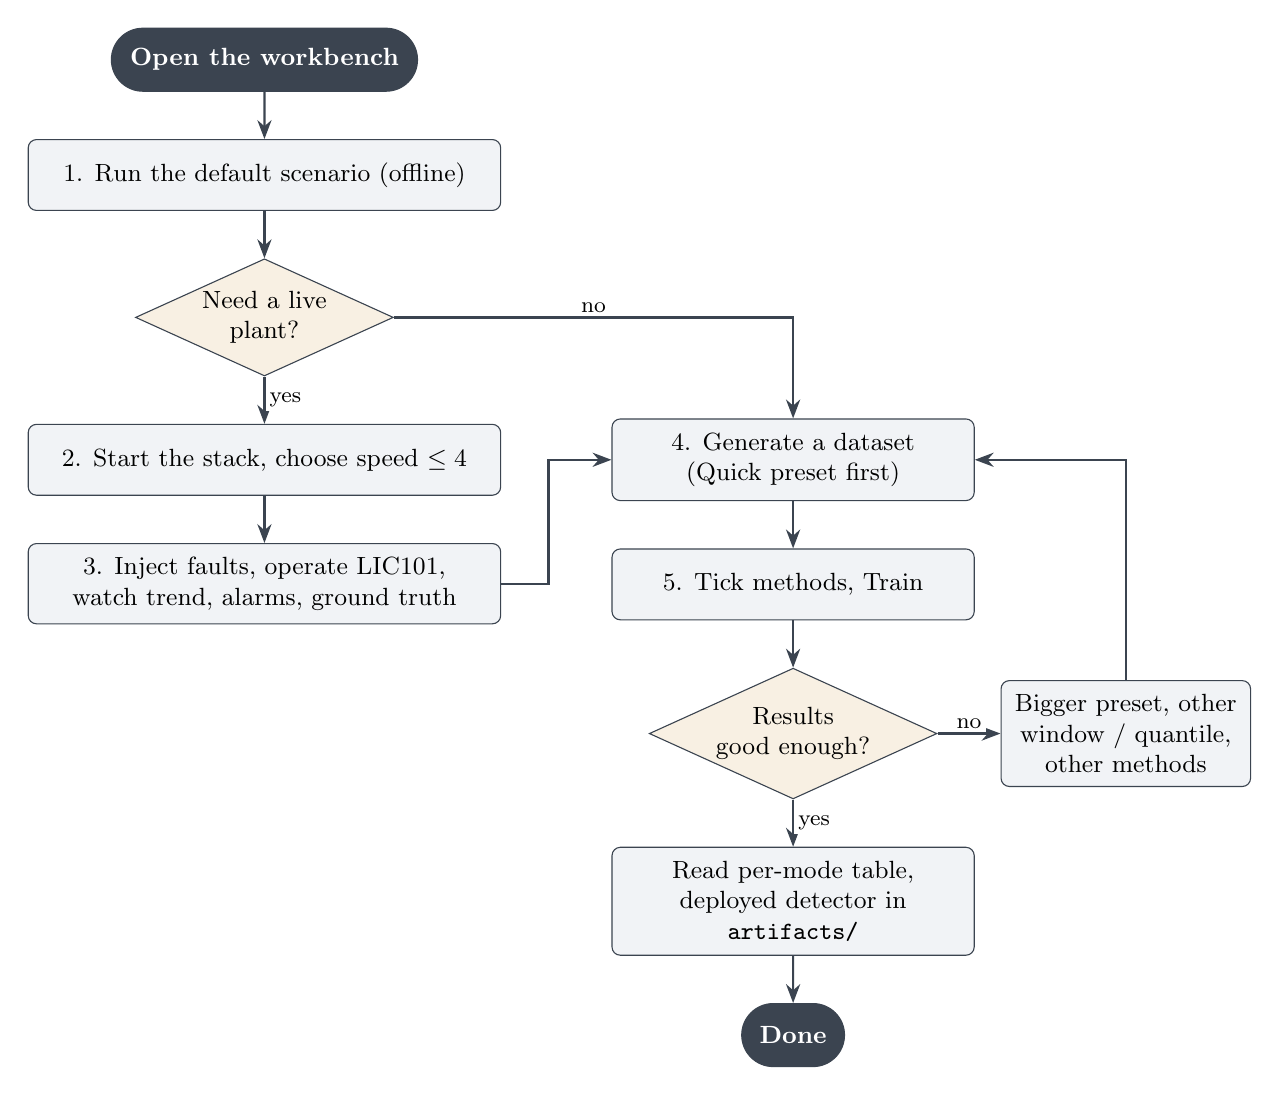
\begin{tikzpicture}[node distance=6mm and 8mm]
  \node[term] (start) {Open the workbench};
  \node[box,below=of start,minimum width=60mm] (s1) {1. Run the default scenario (offline)};
  \node[decision,below=of s1] (q1) {Need a live\\plant?};
  \node[box,below=of q1,minimum width=60mm] (s2) {2. Start the stack, choose speed $\le 4$};
  \node[box,below=of s2,minimum width=60mm] (s3) {3. Inject faults, operate LIC101,\\watch trend, alarms, ground truth};
  \node[box,right=14mm of s2,minimum width=46mm] (s4) {4. Generate a dataset\\(Quick preset first)};
  \node[box,below=of s4,minimum width=46mm] (s5) {5. Tick methods, Train};
  \node[decision,below=of s5] (q2) {Results\\good enough?};
  \node[box,below=of q2,minimum width=46mm] (s6) {Read per-mode table,\\deployed detector in\\\code{artifacts/}};
  \node[box,right=8mm of q2,minimum width=30mm] (tune) {Bigger preset, other\\window / quantile,\\other methods};
  \node[term,below=of s6] (end) {Done};
  \draw[flow] (start) -- (s1);
  \draw[flow] (s1) -- (q1);
  \draw[flow] (q1) -- node[lbl,right]{yes} (s2);
  \draw[flow] (q1.east) -| node[lbl,pos=0.25,above]{no} (s4.north);
  \draw[flow] (s2) -- (s3);
  \draw[flow] (s3.east) -- ++(6mm,0) |- (s4.west);
  \draw[flow] (s4) -- (s5);
  \draw[flow] (s5) -- (q2);
  \draw[flow] (q2) -- node[lbl,right]{yes} (s6);
  \draw[flow] (q2) -- node[lbl,above]{no} (tune);
  \draw[flow] (tune.north) |- (s4.east);
  \draw[flow] (s6) -- (end);
\end{tikzpicture}}
\caption{Recommended workflow through the toolbox.}
\label{fig:workflow}
\end{figure}

\section{Tutorial 1: the default scenario}

\begin{enumerate}
  \item Start the workbench and open \url{http://127.0.0.1:8050}. The Quick
        start tab opens and the default leak scenario runs by itself.
  \item Read the summary cards. With the setpoint held, \tg{LT101} ends where
        it started ($\pm0.1$\,mm) while the controller output rises by about
        9.6\%. This is the central fact of the project: in a closed loop the
        controller absorbs the fault, so the measurement alone does not show
        it.
  \item Choose \ui{Sticking control valve}, length \ui{1 hour}, and press
        \ui{Run scenario}. After onset the level starts to hunt and the
        orange controller output and the green stem position stop agreeing:
        the valve is stuck until the command moves far enough, then jumps.
  \item Choose \ui{LT101 frozen}, tick \ui{setpoint moves}, and run. After
        the setpoint changes the controller chases a reading that cannot
        follow, winds the valve shut, starves the pump, and the minimum-flow
        interlock trips. The \ui{Pump trip} card shows when.
\end{enumerate}

\section{Tutorial 2: the live plant}

\begin{enumerate}
  \item Set \ui{Speed} to $1\times$ or $2\times$ (at most $4\times$ on
        Windows) and press \ui{Start stack}. After about ten seconds the
        services pill reads \ui{4/4 services}.
  \item Open the Runtime tab. The plant starts lined out at its design point:
        \tg{LT101} $\approx$ 300\,mm, valve $\approx$ 66\%, flow
        $\approx$ 10\,L/min, pump pressure $\approx$ 50\,kPa.
  \item \textbf{Setpoint step.} Type 350 in \ui{Setpoint} and press
        \ui{Write}. The level rises to 350\,mm in about 40\,s with no
        overshoot (IMC tuning, Section~\ref{sec:imc}).
  \item \textbf{Manual mode.} Press \ui{Manual}, write 50 to \ui{Manual OP}.
        The valve closes to 50\% and the level falls; the controller is not
        acting. Press \ui{Auto}: the output continues from 50\% without a jump
        (bumpless transfer) and the level returns to setpoint.
  \item \textbf{Rejected write.} Write 3000 to \ui{Setpoint}. The HMI refuses
        it with an error message instead of clamping it silently.
  \item \textbf{Interlock.} Press pump \ui{Stop} and then \ui{Start} while
        watching the alarms, or raise the setpoint to 560\,mm so the level
        crosses the 550\,mm trip. The interlock latches, the pump stops and
        the valve closes. Restore a normal setpoint and press
        \ui{Reset interlock}.
\end{enumerate}

\section{Tutorial 3: faults on the live plant}

\begin{enumerate}
  \item Open the Faults tab and press \ui{Leak in tank 1}. The active-fault
        list shows the new fault; the ground-truth table shows readings equal
        to the true values, because a leak is a process fault and the
        instruments are honest.
  \item On the Runtime tab, the controller output climbs by about 10\% over a
        minute while the level holds.
  \item Press \ui{Clear all faults}, then \ui{LT101 reads 25 mm high}. Now the
        ground-truth table shows \tg{LT101} reported 25\,mm above its true
        value. The controller drives the \emph{reading} back to 300\,mm, so
        the true level sits 25\,mm low and \tg{LT102} falls.
  \item Try \ui{Sticking valve} at $4\times$ speed for a few minutes and
        watch \tg{LIC101_OP} and \tg{ZT101} on the mimic diverge.
  \item Use \ui{Or build one} to inject, for example, \code{pump_wear} with
        magnitude 0.3 and ramp 300\,s, and watch \tg{PT101} fall below what
        the pump curve predicts.
\end{enumerate}

\section{Tutorial 4: a dataset}

\begin{enumerate}
  \item Open the Data tab and press \ui{Quick (\textasciitilde 1.5 min)}.
        The fields become 1200\,s, 1 magnitude, 1 repeat, 6 normal runs.
  \item Press \ui{Generate}. The progress bar fills; when it finishes,
        \ui{Recent runs} shows a \code{dataset} row with the number of runs
        and samples, and \code{dataset.parquet} appears in the workspace.
  \item For publishable numbers use \ui{Standard} (58 runs of an hour) or
        \ui{Thorough}.
\end{enumerate}

The dataset is generated offline, in plant time, with the same code as the
live plant (Figure~\ref{fig:paths}). Each row is one second of one run and
carries all signals, the label, the fault kind, target, onset and ramp.

\section{Tutorial 5: training and comparing detectors}

\begin{enumerate}
  \item Open the Model tab. Leave all four methods ticked, window 60,
        stride 10, quantile 0.995, and press \ui{Train}.
  \item When the bar is full, the Results table compares the methods. The
        method with the highest detection rate is deployed; ties go to the one
        with fewer false alarms and then to the simpler method.
  \item Read the \ui{By fault mode} table. For leak, pump wear, stiction and
        fouling the \ui{expected} column names the physics channel the fault
        should implicate; a match is an isolated fault.
  \item The deployed detector is \code{artifacts/detector.joblib} with its
        \code{manifest.json}; every method's detector and per-run CSV are kept
        beside it.
\end{enumerate}

On the Quick dataset, a typical result is:

\begin{center}
\begin{tabular}{@{}lrrrr@{}}
\toprule
Method & Detected & Median delay & False alarms/day & Isolation \\
\midrule
Z-score limits & 62.5\% & 341\,s & 0.00 & 100\% \\
PCA / MSPC & 87.5\% & 43\,s & 0.00 & 80\% \\
Isolation forest & 37.5\% & 354\,s & 0.00 & 100\% \\
Autoencoder & 87.5\% & 43\,s & 0.00 & 60\% \\
\bottomrule
\end{tabular}
\end{center}

On the Standard dataset the README reports the autoencoder at 100\%
detection with a 70\,s median delay and PCA at 83\% with 256\,s. Small
datasets favour simple models; larger ones let the learned model pull ahead.

\section{Tutorial 6: the same pipeline from Python}

Everything the workbench does is available as functions:

\begin{lstlisting}
from pyplant.workbench.tasks import (run_default_scenario,
                                     generate_dataset, train_detector)

result = run_default_scenario("stiction", duration=3600.0)
print(result["onset"], result["series"]["LIC101_OP"][-1])

noop = lambda fraction, message="": None      # progress callback
generate_dataset(noop, "./work/scratch", duration=1200.0,
                 magnitudes=1, repeats=1, normal_runs=6)
summary = train_detector(noop, "./work/scratch",
                         methods=["zscore", "pca"])
print(summary["selected"], summary["results"]["pca"]["detection_rate"])
\end{lstlisting}

And the command-line training pipeline of the README:

\begin{lstlisting}[style=sh]
python -m pyplant.ml.train --out artifacts --duration 3600 \
       --magnitudes 3 --repeats 2 --normal-runs 6 --window 60 --stride 10
\end{lstlisting}

\chapter{The plant model}
\label{ch:plant}

\code{pyplant/core/hybrid_tank.py} holds the physics as pure functions: SI
units throughout, no sockets, no sleeping, no global state. This chapter
derives every equation it implements.

\section{State, inputs and outputs}

The state vector is
\[
  \bm{x} = \begin{bmatrix} h_1 & h_2 & z \end{bmatrix}^\top,
\]
the two levels in metres and the valve stem position $z\in[0,1]$. The inputs
are the valve command $u\in[0,1]$ and the pump run command. The outputs are
the instrument readings of Table~\ref{tab:meas}.

\begin{table}[htbp]
\centering
\begin{tabular}{@{}llll@{}}
\toprule
Tag & Quantity & Formula & Span \\
\midrule
\tg{LT101} & tank 1 level & $1000\,h_1$ & 0--600\,mm \\
\tg{LT102} & tank 2 level & $1000\,h_2$ & 0--600\,mm \\
\tg{FT101} & pump discharge flow & $60\,000\,q_\text{in}$ & 0--20\,L/min \\
\tg{FT102} & tank 2 outlet flow & $60\,000\,q_\text{out}$ & 0--20\,L/min \\
\tg{PT101} & pump discharge pressure & $p_\text{pump}/1000$ & 0--100\,kPa \\
\tg{ZT101} & valve stem position & $100\,z$ & 0--100\,\% \\
\tg{PMP101_RUN} & pump running feedback & pump command & bool \\
\bottomrule
\end{tabular}
\caption{Measurements. \code{measure()} is the only function that converts SI
to engineering units.}
\label{tab:meas}
\end{table}

\section{Mass balances}

Each tank is a vertical cylinder of cross-section $A$. Conservation of volume
for an incompressible liquid gives
\begin{align}
  A_1 \frac{dh_1}{dt} &= q_\text{in} - q_{12} - q_\text{leak}, \label{eq:tank1}\\
  A_2 \frac{dh_2}{dt} &= q_{12} - q_\text{out}. \label{eq:tank2}
\end{align}
Both tanks are bounded: a level at the overflow lip $h_\text{max}=0.6$\,m
cannot rise further, and an empty tank cannot drain.

\section{Gravity drains: Torricelli's law}

Flow through an orifice under a head $h$ follows from Bernoulli's equation
between the free surface and the jet, $v=\sqrt{2gh}$, multiplied by an
effective discharge area $C_dA$ that lumps the geometric area and the
contraction coefficient:
\begin{equation}
  q = C_dA\,\sqrt{2gh}.
\end{equation}
This gives the interconnect, outlet and leak flows:
\begin{align}
  q_{12} &= C_dA_{12}\,g_{12}\,\sqrt{2gh_1}, &
  q_\text{out} &= C_dA_{2,\text{out}}\,\sqrt{2gh_2}, &
  q_\text{leak} &= C_dA_\text{leak}\,\sqrt{2gh_1},
\end{align}
where $g_{12}\le1$ is the fouling factor and $C_dA_\text{leak}\ge0$ the leak
area. Both are healthy at $g_{12}=1$, $C_dA_\text{leak}=0$.

\section{Pump and valve: an algebraic loop solved in closed form}

A centrifugal pump develops less pressure as it delivers more flow. A
quadratic curve is the standard approximation:
\begin{equation}
  p_\text{pump} = \Delta p_0\,\gamma\left(1-\left(\frac{q}{q_\text{max}}\right)^2\right),
\end{equation}
with shut-off pressure $\Delta p_0 = 60$\,kPa, run-out flow
$q_\text{max} = 25$\,L/min and wear factor $\gamma\le1$.

The control valve passes a flow proportional to the square root of the
pressure drop across it. The drop is the pump pressure minus the static head
of tank~1:
\begin{equation}
  q = k\sqrt{p_\text{pump}-\rho g h_1}, \qquad k = C_v\,\phi(z).
\end{equation}

The valve has an \emph{equal-percentage} inherent characteristic with
rangeability $R=30$: equal increments of stem travel change the flow by equal
percentages,
\begin{equation}
  \phi(z) = R^{\,z-1}, \qquad \phi(1) = 1,\ \phi(0) = 1/R,
\end{equation}
and below a seat position of 0.5\% the valve shuts tight. Under a falling
pump curve, an equal-percentage valve gives a roughly linear
\emph{installed} characteristic, which is why it is chosen.

Pump pressure depends on flow, and flow depends on pump pressure. Substituting
one into the other and solving the quadratic gives
\begin{equation}
  \boxed{\;q_\text{in} = k\sqrt{\dfrac{\Delta p_0\gamma - \rho g h_1}
        {1 + k^2\,\Delta p_0\gamma/q_\text{max}^2}}\;}
  \label{eq:qin}
\end{equation}
so no iteration is needed and the system is not stiff at a 50\,ms step. If the
valve is shut the pump dead-heads at $\Delta p_0\gamma$; if the pump is off,
$q_\text{in}=0$.

\begin{figure}[htbp]
\centering
\begin{subfigure}{0.4\textwidth}
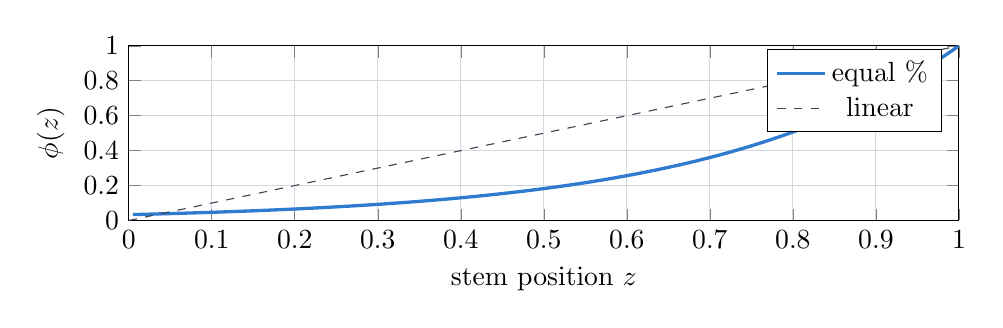
\begin{tikzpicture}
\begin{axis}[width=\textwidth,height=3.8cm,xlabel={stem position $z$},
  ylabel={$\phi(z)$},grid=major,grid style={linegrey},
  xmin=0,xmax=1,ymin=0,ymax=1]
\addplot[accent,very thick,domain=0.005:1,samples=80]{30^(x-1)};
\addplot[slate,dashed,domain=0:1]{x};
\legend{equal \%, linear}
\end{axis}
\end{tikzpicture}
\caption{Inherent valve characteristic, $R=30$.}
\end{subfigure}\hfill
\begin{subfigure}{0.4\textwidth}
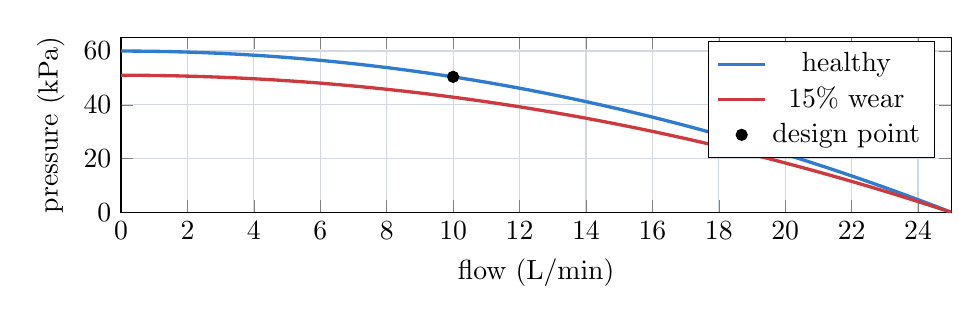
\begin{tikzpicture}
\begin{axis}[width=\textwidth,height=3.8cm,xlabel={flow (L/min)},
  ylabel={pressure (kPa)},grid=major,grid style={linegrey},
  xmin=0,xmax=25,ymin=0,ymax=65]
\addplot[accent,very thick,domain=0:25,samples=60]{60*(1-(x/25)^2)};
\addplot[badred,very thick,domain=0:25,samples=60]{0.85*60*(1-(x/25)^2)};
\addplot[only marks,mark=*,mark size=2pt] coordinates {(10,50.4)};
\legend{healthy,15\% wear,design point}
\end{axis}
\end{tikzpicture}
\caption{Pump curve, healthy and worn.}
\end{subfigure}
\caption{Component characteristics used by the plant model.}
\label{fig:curves}
\end{figure}

\section{Valve actuator}

The stem follows the command through a first-order lag with
$\tau_v = 2$\,s:
\begin{equation}
  \tau_v \frac{dz}{dt} = u - z .
\end{equation}

\section{Numerical integration}

The model is integrated with the classical fourth-order Runge--Kutta method at
$\Delta t = 50$\,ms:
\begin{align*}
  \bm k_1 &= f(\bm x_n,u), &
  \bm k_2 &= f(\bm x_n + \tfrac{\Delta t}{2}\bm k_1,u),\\
  \bm k_3 &= f(\bm x_n + \tfrac{\Delta t}{2}\bm k_2,u), &
  \bm k_4 &= f(\bm x_n + \Delta t\,\bm k_3,u),\\
  \bm x_{n+1} &= \bm x_n + \tfrac{\Delta t}{6}(\bm k_1+2\bm k_2+2\bm k_3+\bm k_4),
\end{align*}
after which levels are clipped to $[0,h_\text{max}]$ and $z$ to $[0,1]$. The
input is held constant within a step.

\section{Steady state}

At equilibrium $dh_1/dt = 0$. For a fixed valve position, inflow falls and
outflow rises monotonically with $h_1$, so the residual
$r(h_1) = q_\text{in} - q_{12} - q_\text{leak}$ has a single root, found by
bisection. Then $dh_2/dt=0$ gives tank 2 directly:
\begin{equation}
  h_2 = \frac{1}{2g}\left(\frac{q_{12}}{C_dA_{2,\text{out}}}\right)^2 .
\end{equation}
\code{steady_state()} is used to start the plant lined out and by the tests.

\section{Sizing and the design point}

\begin{table}[htbp]
\centering
\begin{tabular}{@{}lll@{}}
\toprule
Parameter (\code{Params} field) & Value & Meaning \\
\midrule
\code{area_tank1}, \code{area_tank2} & 0.020\,m$^2$ & tank cross-sections ($\approx$160\,mm diameter) \\
\code{height_max} & 0.600\,m & overflow lip \\
\code{pump_dp0} & 60\,000\,Pa & shut-off pressure \\
\code{pump_qmax} & $4.17\times10^{-4}$\,m$^3$/s & run-out flow, 25\,L/min \\
\code{valve_cv} & $2.429\times10^{-6}$ & valve coefficient fully open, m$^3$/(s$\sqrt{\text{Pa}}$) \\
\code{valve_rangeability} & 30 & equal-percentage $R$ \\
\code{valve_seat} & 0.005 & tight shut-off below this position \\
\code{tau_valve} & 2.0\,s & actuator lag \\
\code{cda_12} & $6.90\times10^{-5}$\,m$^2$ & tank 1 to tank 2 orifice \\
\code{cda_2out} & $9.00\times10^{-5}$\,m$^2$ & tank 2 drain \\
\code{pump_gain} & 1.0 & fault knob: $<1$ is impeller wear \\
\code{cda_12_gain} & 1.0 & fault knob: $<1$ is fouling \\
\code{cda_leak} & 0.0 & fault knob: leak area \\
\bottomrule
\end{tabular}
\caption{Plant parameters and their defaults.}
\label{tab:params}
\end{table}

At the design point the valve is 66\% open, the level is 300\,mm, the flow
10\,L/min and the pump pressure 50\,kPa. The usable level range is roughly 30
to 580\,mm, corresponding to valve positions from 0.30 to 0.79.

\section{Linearisation and the process time constant}

Tuning needs a linear model. Around an operating point $(\bar h_1,\bar z)$,
write $h_1 = \bar h_1 + \delta h$, $z = \bar z + \delta z$ and expand
equation~\eqref{eq:tank1} to first order:
\begin{equation}
  A_1 \frac{d\,\delta h}{dt}
   = \underbrace{\left(\frac{\partial q_\text{in}}{\partial h_1}
     - \frac{\partial q_{12}}{\partial h_1}\right)}_{-1/R_h}\delta h
   + \frac{\partial q_\text{in}}{\partial z}\,\delta z .
\end{equation}
Inflow falls as the back-pressure rises, so $\partial q_\text{in}/\partial h_1<0$,
and outflow rises with head, $\partial q_{12}/\partial h_1 = q_{12}/(2h_1)>0$;
the bracket is therefore negative and the tank is self-regulating. This is a
first-order system
\begin{equation}
  \tau \frac{d\,\delta h}{dt} + \delta h = K\,\delta z,
  \qquad \tau = A_1 R_h,\quad K = R_h\frac{\partial q_\text{in}}{\partial z}.
\end{equation}
An open-loop step test on the model at the design point gives
$K \approx 15.4$\,mm per \% of valve travel and $\tau\approx 72$\,s, the
values the controller is tuned for. The valve lag (2\,s) is small compared
with $\tau$ and is neglected in tuning.

\begin{figure}[htbp]
\centering
\scalebox{0.8}{%
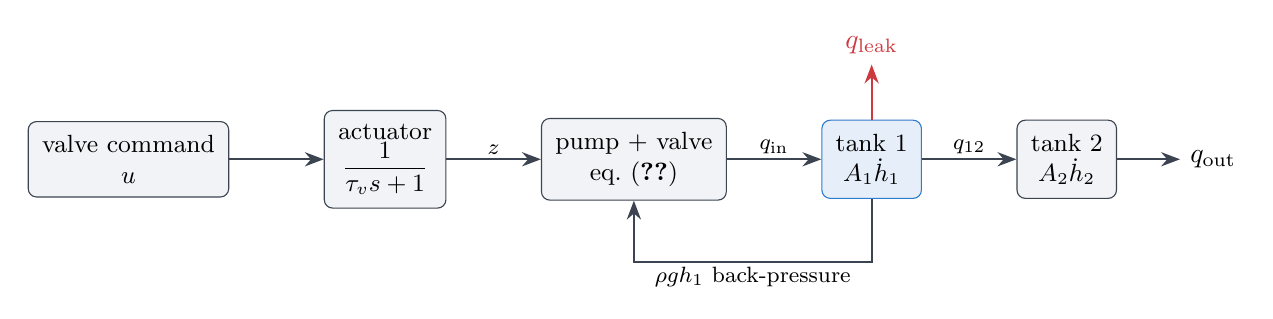
\begin{tikzpicture}[node distance=12mm]
  \node[box] (u) {valve command\\$u$};
  \node[box,right=of u] (v) {actuator\\$\dfrac{1}{\tau_v s+1}$};
  \node[box,right=of v] (q) {pump + valve\\eq.~\eqref{eq:qin}};
  \node[hot,right=of q] (t1) {tank 1\\$A_1\dot h_1$};
  \node[box,right=of t1] (t2) {tank 2\\$A_2\dot h_2$};
  \draw[flow] (u) -- (v);
  \draw[flow] (v) -- node[lbl,above]{$z$} (q);
  \draw[flow] (q) -- node[lbl,above]{$q_\text{in}$} (t1);
  \draw[flow] (t1) -- node[lbl,above]{$q_{12}$} (t2);
  \draw[flow] (t1.south) -- ++(0,-8mm) -| node[lbl,pos=0.25,below]{$\rho g h_1$ back-pressure} (q.south);
  \draw[flow] (t2.east) -- ++(8mm,0) node[right]{$q_\text{out}$};
  \draw[flow,badred] (t1.north) -- ++(0,7mm) node[above]{$q_\text{leak}$};
\end{tikzpicture}}
\caption{Signal flow inside the plant model.}
\label{fig:plant-signal}
\end{figure}

\section{The simulation stepper}

\code{pyplant/runners/base.py} holds \code{Simulation}, the one loop body both
runners drive. It has three deliberately different rates:

\begin{center}
\begin{tabular}{@{}lll@{}}
\toprule
Rate & Default & What it governs \\
\midrule
\code{dt} & 50\,ms & integration accuracy \\
\code{control_period} & 100\,ms & how often the controller sees the plant \\
\code{log_period} & 1\,s & what the historian and datasets store \\
\bottomrule
\end{tabular}
\end{center}

The controller period must be a whole number of integration steps, and time
is computed from an integer step count rather than by repeated addition, so it
never accumulates rounding error. Between controller executions the inputs
are held: a genuine zero-order hold, as on a real PLC. Faults are applied in
\code{Simulation.integrate()}, the single place both runners share
(Chapter~\ref{ch:faults}).

\chapter{Control theory and the LIC101 loop}
\label{ch:control}

This chapter explains feedback control from first principles and then the
specific controller in \code{pyplant/plc/pid.py}: a velocity-form PID with
structural anti-windup, bumpless transfer, derivative on filtered measurement
and IMC tuning.

\section{Feedback control}

A feedback loop measures the controlled variable (the \emph{process value},
PV), compares it with the desired value (the \emph{setpoint}, SP), and moves
a manipulated variable (the \emph{controller output}, OP) to remove the
difference $e = \text{SP} - \text{PV}$. Figure~\ref{fig:loop} shows LIC101 in
this form.

\begin{figure}[htbp]
\centering
\scalebox{0.8}{%
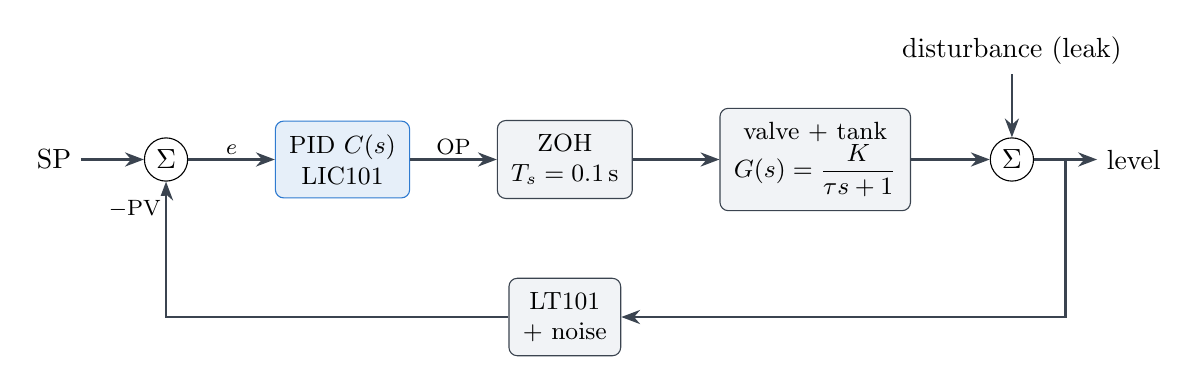
\begin{tikzpicture}[node distance=11mm]
  \node (sp) {SP};
  \node[circle,draw,right=8mm of sp,inner sep=2pt] (sum) {$\Sigma$};
  \node[hot,right=of sum] (c) {PID $C(s)$\\LIC101};
  \node[box,right=of c] (zoh) {ZOH\\$T_s=0.1$\,s};
  \node[box,right=of zoh] (p) {valve + tank\\$G(s)=\dfrac{K}{\tau s+1}$};
  \node[circle,draw,right=10mm of p,inner sep=2pt] (dsum) {$\Sigma$};
  \node[right=8mm of dsum] (pv) {level};
  \node[above=8mm of dsum] (d) {disturbance (leak)};
  \node[box,below=10mm of zoh] (m) {LT101\\+ noise};
  \draw[flow] (sp) -- (sum);
  \draw[flow] (sum) -- node[lbl,above]{$e$} (c);
  \draw[flow] (c) -- node[lbl,above]{OP} (zoh);
  \draw[flow] (zoh) -- (p);
  \draw[flow] (p) -- (dsum);
  \draw[flow] (d) -- (dsum);
  \draw[flow] (dsum) -- (pv);
  \draw[flow] ($(dsum.east)+(4mm,0)$) |- (m);
  \draw[flow] (m) -| node[lbl,pos=0.9,left]{$-$PV} (sum);
\end{tikzpicture}}
\caption{LIC101 as a feedback loop. The PLC samples the level every 100\,ms and
holds its output between scans.}
\label{fig:loop}
\end{figure}

\section{The PID law}

The ideal continuous PID controller in standard (ISA) form is
\begin{equation}
  u(t) = K_c\left( e(t) + \frac{1}{T_i}\int_0^t e(\tau)\,d\tau
         + T_d\frac{de}{dt}\right),
\end{equation}
with controller gain $K_c$, integral time $T_i$ and derivative time $T_d$. Each
term has a role:
\begin{description}
  \item[Proportional] reacts to the present error. Alone it leaves a steady
        offset whenever a non-zero output is needed to hold the setpoint.
  \item[Integral] accumulates past error and keeps moving the output until
        the error is exactly zero. It removes offset, and it is the reason a
        leak is masked (Section~\ref{sec:masking}).
  \item[Derivative] anticipates by reacting to the rate of change. On a noisy
        level it does more harm than good, so LIC101 runs with $T_d=0$.
\end{description}

\subsection{Positional and velocity forms}

Discretising at sample time $T_s$ with backward differences gives the
\emph{positional} form
\begin{equation}
  u_k = K_c\Big(e_k + \frac{T_s}{T_i}\sum_{j\le k} e_j
        + \frac{T_d}{T_s}(e_k - e_{k-1})\Big).
\end{equation}
Subtracting $u_{k-1}$ from $u_k$ gives the \emph{velocity} (incremental) form
used here:
\begin{equation}
  \Delta u_k = K_c(e_k - e_{k-1}) + K_c\frac{T_s}{T_i}e_k
   - K_c\frac{T_d}{T_s}\big(y^f_k - 2y^f_{k-1} + y^f_{k-2}\big),
  \qquad u_k = \operatorname{clip}\big(u_{k-1} + \Delta u_k,\,0,\,100\big),
  \label{eq:velocity}
\end{equation}
where $y^f$ is the filtered measurement (below). For a reverse-acting loop the
derivative term has a minus sign because it acts on the measurement.

\subsection{Why the velocity form}

In the velocity form the output itself is the integrator state. Two
properties that need extra logic in the positional form become automatic:

\begin{theory}[Anti-windup is structural]
When the actuator saturates, a positional PID keeps integrating the error, so
the integral grows far beyond the limit (\emph{windup}) and the output stays
pinned long after the error reverses. In equation~\eqref{eq:velocity} the
increment that would push past a limit is simply clipped away. No hidden
accumulator grows, and the output leaves the limit on the first scan the
error changes sign.
\end{theory}

\begin{theory}[Bumpless transfer is structural]
In manual mode the output is whatever the operator writes, and the controller
keeps its error history fresh against the current PV (\code{track()}). On
return to auto it continues incrementing from the manual value, so the valve
does not jump.
\end{theory}

\subsection{Derivative on filtered measurement}

Taking the derivative of the error differentiates the setpoint too, so a
setpoint step would produce an impulse (\emph{derivative kick}). The code
differentiates the measurement instead. The measurement is first passed
through a first-order low-pass filter with time constant $T_f = 5$\,s,
discretised as
\begin{equation}
  y^f_k = y^f_{k-1} + \alpha\,(y_k - y^f_{k-1}),
  \qquad \alpha = \frac{T_s}{T_f + T_s}.
\end{equation}

\subsection{Initialisation from valve feedback}

A velocity PID increments from wherever its output already is. Starting at
0\% would slam shut the valve of a plant running at 66\%, dead-head the pump
and trip the interlock on the first scan. On the first scan the program
therefore seeds the output from the measured stem position \tg{ZT101}.

\section{IMC tuning}
\label{sec:imc}

Internal Model Control (IMC) tuning chooses the controller so that the closed
loop behaves like a first-order lag with a time constant $\lambda$ the
engineer specifies. For a first-order process
\begin{equation}
  G(s) = \frac{K}{\tau s + 1},
\end{equation}
the IMC controller is $Q(s) = G^{-1}(s)\,\frac{1}{\lambda s+1}$ and the
equivalent feedback controller is
\begin{equation}
  C(s) = \frac{Q}{1 - GQ} = \frac{\tau s + 1}{K\lambda s}
       = \frac{\tau}{K\lambda}\left(1 + \frac{1}{\tau s}\right),
\end{equation}
which is a PI controller with
\begin{equation}
  \boxed{K_c = \frac{\tau}{K\lambda}, \qquad T_i = \tau .}
\end{equation}
The integral time cancels the process pole, and the closed-loop response to a
setpoint step is
\begin{equation}
  \frac{\text{PV}(s)}{\text{SP}(s)} = \frac{GC}{1+GC} = \frac{1}{\lambda s+1}.
\end{equation}

For LIC101, $K = 15.4$\,mm/\%, $\tau = 72$\,s and $\lambda = 13$\,s:
\[
  K_c = \frac{72}{15.4\times13} \approx 0.36 \;\to\; 0.35\ \%/\text{mm},
  \qquad T_i = 72\ \text{s}, \qquad T_d = 0.
\]
The ratio $\tau/\lambda\approx5.5$ gives a closed loop five times faster than
the open loop while leaving margin for the neglected valve lag, the sample
time and the nonlinearity.

\begin{figure}[htbp]
\centering
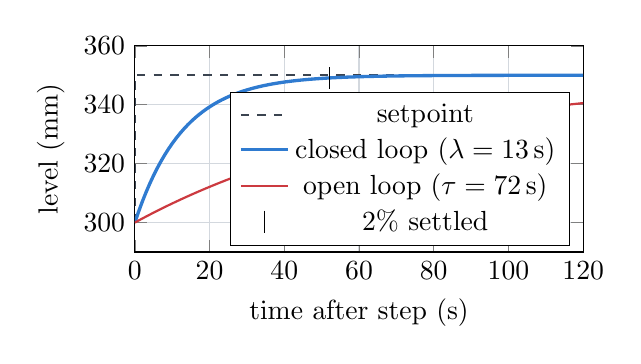
\begin{tikzpicture}
\begin{axis}[width=0.6\textwidth,height=4.2cm,xlabel={time after step (s)},
  ylabel={level (mm)},grid=major,grid style={linegrey},xmin=0,xmax=120,
  ymin=290,ymax=360,legend pos=south east]
\addplot[slate,dashed,thick] coordinates {(0,300)(0,350)(120,350)};
\addplot[accent,very thick,domain=0:120,samples=120]{300+50*(1-exp(-x/13))};
\addplot[badred,thick,domain=0:120,samples=120]{300+50*(1-exp(-x/72))};
\addplot[only marks,mark=|,mark size=4pt] coordinates {(52,349)};
\legend{setpoint, closed loop ($\lambda=13$\,s), open loop ($\tau=72$\,s), 2\% settled}
\end{axis}
\end{tikzpicture}
\caption{Ideal response to a 50\,mm setpoint step. The measured response of
the real loop matches: no overshoot, 2\% settling in about 40--50\,s, zero
offset.}
\label{fig:step}
\end{figure}

\section{Sampling and the zero-order hold}

The PLC executes every $T_s = 100$\,ms and holds its output until the next
scan. A zero-order hold behaves approximately like a dead time of $T_s/2 =
50$\,ms, negligible against $\lambda = 13$\,s, but it is modelled physically
rather than ignored: the simulator integrates at 50\,ms with the input held
between scans. A PID that looks better in simulation than on a PLC usually
lacks exactly this.

\section{Why integral action hides a leak}
\label{sec:masking}

A leak is a load disturbance $d$ on tank~1. With a PI controller the
steady-state error to a step disturbance is, by the final value theorem,
\begin{equation}
  e_\infty = \lim_{s\to0} s\cdot\frac{G_d(s)}{1+G(s)C(s)}\cdot\frac{d}{s} = 0,
\end{equation}
because $C(s)$ has a pole at $s=0$. The controller drives the level back to
setpoint exactly, and the only lasting evidence is that the output has moved:

\begin{center}
\begin{tabular}{@{}lrr@{}}
\toprule
& \tg{LT101} & \tg{LIC101_OP} \\
\midrule
before the leak & 300.00\,mm & 66.18\% \\
after the leak & 300.00\,mm & 75.80\% \\
\bottomrule
\end{tabular}
\end{center}

A diagnosis model fed only the process value cannot see this fault. This is
why the detectors are given the controller output, the valve position and
derived physics channels (Chapter~\ref{ch:ml}).

\section{Controller parameters}

\begin{center}
\begin{tabular}{@{}llll@{}}
\toprule
\code{PidTuning} field & Default & Unit & Meaning \\
\midrule
\code{kc} & 0.35 & \%/mm & controller gain \\
\code{ti} & 72.0 & s & integral time (0 disables integral action) \\
\code{td} & 0.0 & s & derivative time (0 disables derivative) \\
\code{tf} & 5.0 & s & derivative filter time constant \\
\code{out_lo}, \code{out_hi} & 0, 100 & \% & output limits \\
\code{direct_acting} & False & & False: output rises when PV falls \\
\bottomrule
\end{tabular}
\end{center}

Chapter~\ref{ch:params} explains how to change them.

\chapter{The soft PLC}
\label{ch:plc}

A programmable logic controller is a computer built to run one program
forever, deterministically, on a fixed cycle. This chapter describes the PLC
model pyplant implements: the scan cycle, the program and its precedence
rules, protective logic, timers, the drift-free scheduler and the
communication layers.

\section{The scan cycle}

Every PLC scan does three things, always in this order:

\begin{enumerate}
  \item \textbf{Read inputs.} All field inputs are copied into an
        \emph{input image table} in one operation.
  \item \textbf{Execute logic.} The program runs against the frozen image.
        It never reads a field value directly, so every rung in one scan sees
        the same consistent snapshot.
  \item \textbf{Write outputs.} The \emph{output image table} is written to
        the field in one operation.
\end{enumerate}

\begin{figure}[htbp]
\centering
\scalebox{0.8}{%
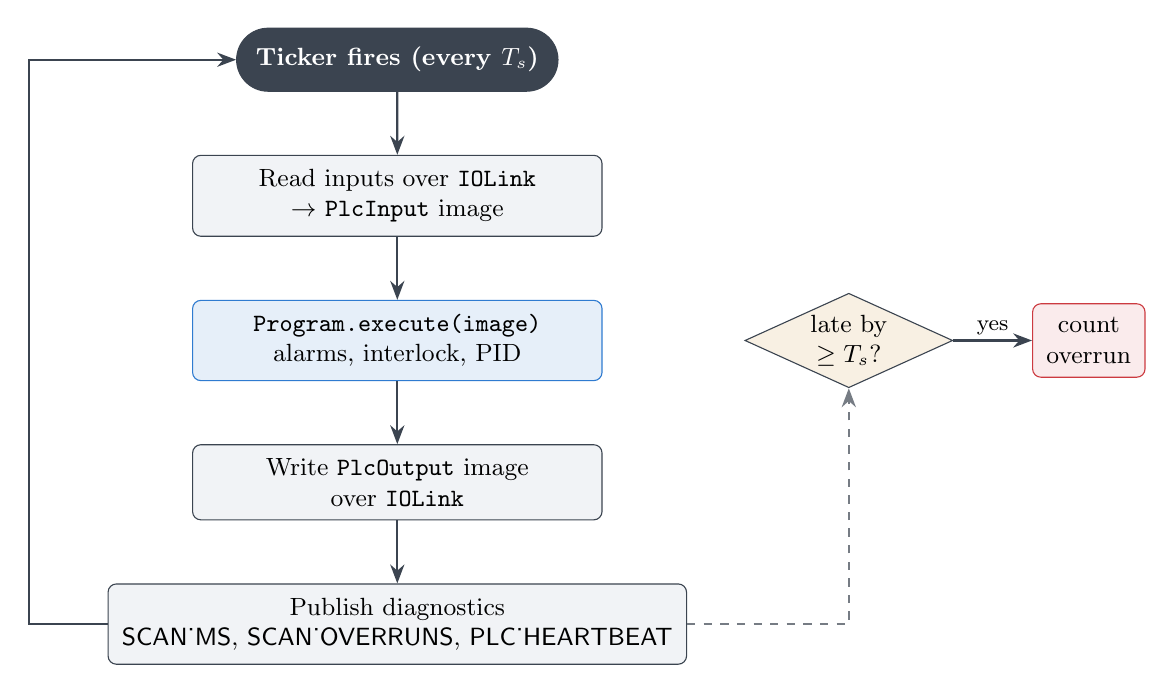
\begin{tikzpicture}[node distance=8mm and 10mm]
  \node[term] (tick) {Ticker fires (every $T_s$)};
  \node[box,below=of tick,minimum width=52mm] (read) {Read inputs over \code{IOLink}\\$\to$ \code{PlcInput} image};
  \node[hot,below=of read,minimum width=52mm] (exec) {\code{Program.execute(image)}\\alarms, interlock, PID};
  \node[box,below=of exec,minimum width=52mm] (write) {Write \code{PlcOutput} image\\over \code{IOLink}};
  \node[box,below=of write,minimum width=52mm] (diag) {Publish diagnostics\\\tg{SCAN_MS}, \tg{SCAN_OVERRUNS}, \tg{PLC_HEARTBEAT}};
  \node[decision,right=18mm of exec] (late) {late by\\$\ge T_s$?};
  \node[bad,right=of late] (ovr) {count\\overrun};
  \draw[flow] (tick) -- (read);
  \draw[flow] (read) -- (exec);
  \draw[flow] (exec) -- (write);
  \draw[flow] (write) -- (diag);
  \draw[flow] (diag.west) -- ++(-10mm,0) |- (tick.west);
  \draw[dflow] (diag.east) -| (late.south);
  \draw[flow] (late) -- node[lbl,above]{yes} (ovr);
\end{tikzpicture}}
\caption{One scan of the PLC engine (\code{pyplant/plc/scan.py}).}
\label{fig:scan}
\end{figure}

The engine (\code{ScanEngine}) does not know whether its I/O is in-process or
Modbus: all I/O goes through the \code{IOLink} protocol. The program
(\code{Program}) does not know about I/O at all: \code{execute()} is a pure
function of the input image and the program's retained state, which is what
makes it testable scan by scan.

\section{The program}

\subsection{Precedence}
Highest first, as on a real unit:
\begin{enumerate}
  \item \textbf{Interlock.} Latched on a trip condition. Forces the pump off,
        drives the valve shut, and keeps the PID tracking 0\% so a reset
        cannot slam the valve open. Clears only when the operator resets
        \emph{and} the condition has gone.
  \item \textbf{Manual.} The operator's output demand passes through; the PID
        tracks it so that returning to auto is bumpless.
  \item \textbf{Auto.} The PID holds \tg{LT101} at \tg{LIC101_SP}.
\end{enumerate}

\begin{figure}[htbp]
\centering
\scalebox{0.8}{%
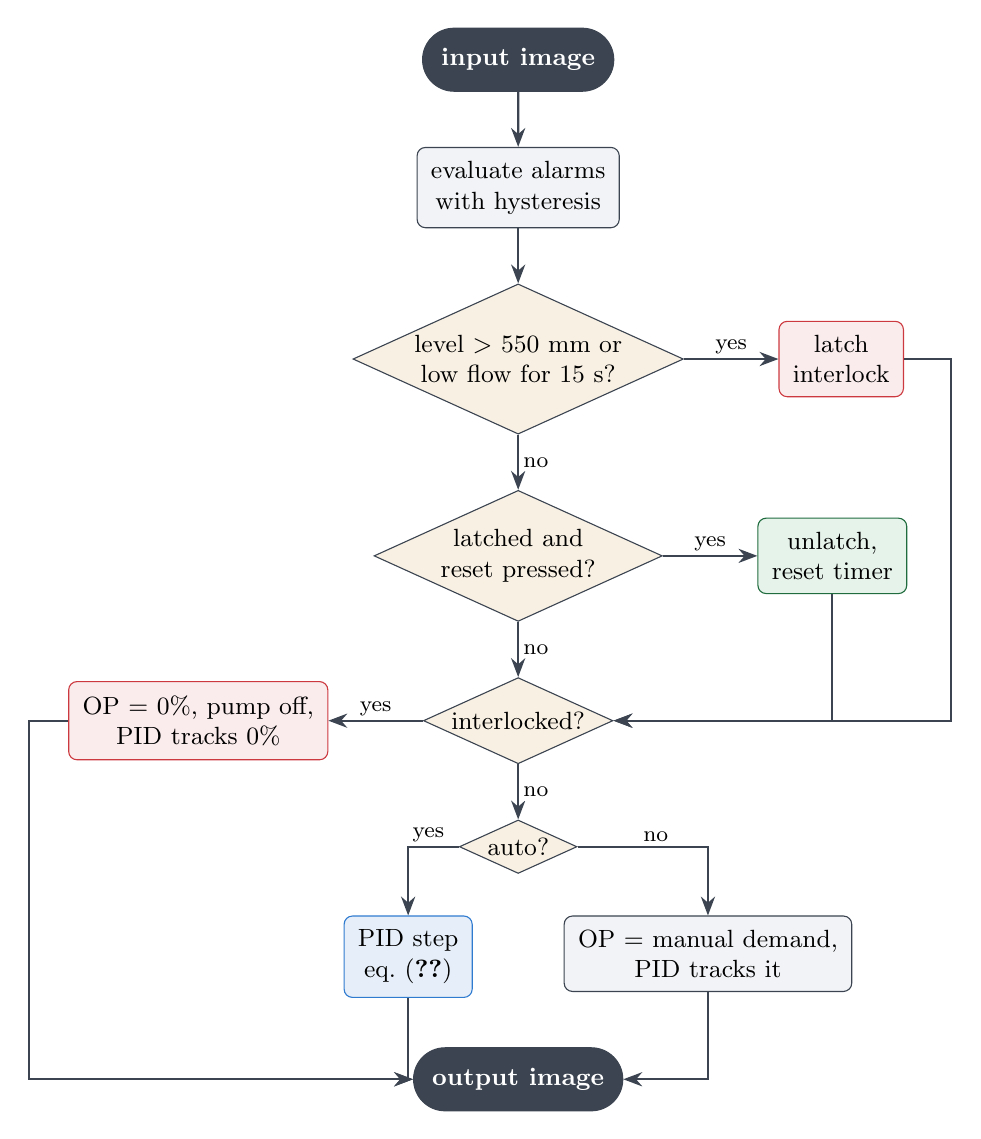
\begin{tikzpicture}[node distance=7mm and 12mm]
  \node[term] (in) {input image};
  \node[box,below=of in] (alm) {evaluate alarms\\with hysteresis};
  \node[decision,below=of alm] (trip) {level $>$ 550 mm or\\low flow for 15 s?};
  \node[bad,right=of trip] (latch) {latch\\interlock};
  \node[decision,below=of trip] (rst) {latched and\\reset pressed?};
  \node[good,right=of rst] (unl) {unlatch,\\reset timer};
  \node[decision,below=of rst] (il) {interlocked?};
  \node[bad,left=of il] (safe) {OP = 0\%, pump off,\\PID tracks 0\%};
  \node[decision,below=of il] (auto) {auto?};
  \node[hot,below left=7mm and 2mm of auto] (pid) {PID step\\eq.~\eqref{eq:velocity}};
  \node[box,below right=7mm and 2mm of auto] (man) {OP = manual demand,\\PID tracks it};
  \node[term,below=22mm of auto] (out) {output image};
  \draw[flow] (in) -- (alm);
  \draw[flow] (alm) -- (trip);
  \draw[flow] (trip) -- node[lbl,above]{yes} (latch);
  \draw[flow] (trip) -- node[lbl,right]{no} (rst);
  \draw[flow] (rst) -- node[lbl,above]{yes} (unl);
  \draw[flow] (rst) -- node[lbl,right]{no} (il);
  \draw[flow] (unl) |- (il);
  \draw[flow] (latch.east) -- ++(6mm,0) |- (il.east);
  \draw[flow] (il) -- node[lbl,above]{yes} (safe);
  \draw[flow] (il) -- node[lbl,right]{no} (auto);
  \draw[flow] (auto) -| node[lbl,pos=0.3,above]{yes} (pid);
  \draw[flow] (auto) -| node[lbl,pos=0.3,above]{no} (man);
  \draw[flow] (pid) |- (out);
  \draw[flow] (man) |- (out);
  \draw[flow] (safe.west) -- ++(-5mm,0) |- (out.west);
\end{tikzpicture}}
\caption{Decision flow of \code{Program.execute()} in one scan.}
\label{fig:program}
\end{figure}

\subsection{Protective functions}

\begin{center}
\begin{tabularx}{\textwidth}{@{}lXX@{}}
\toprule
Function & Trigger & Action \\
\midrule
\tg{ALM_LT101_HI} & \tg{LT101} $>$ 500\,mm & alarm, priority medium \\
\tg{ALM_LT101_LOLO} & \tg{LT101} $<$ 50\,mm & alarm, priority high \\
\tg{ALM_PT101_HIHI} & \tg{PT101} $>$ 58\,kPa & alarm, priority high \\
\tg{ILK_PMP101} & \tg{LT101} $>$ 550\,mm, or \tg{FT101} $<$ 1\,L/min for 15\,s while running & latched trip: pump off, valve shut; priority critical \\
\bottomrule
\end{tabularx}
\end{center}

All thresholds are read from the tag dictionary, so a respanned instrument
cannot leave a stale limit behind in the logic.

\begin{theory}[Why minimum flow and not high pressure]
A centrifugal pump against a shut valve rises to its shut-off head, 60\,kPa
here. A high-pressure trip below that would fire during any legitimate
low-output excursion. The real hazard of dead-heading is that no flow carries
heat away, so the trip is \emph{low flow on a time delay} and high pressure
is only an alarm.
\end{theory}

\subsection{Hysteresis}
A comparator that switches exactly at a limit chatters when the signal rests
on it, and an alarm list that chatters is one operators stop reading. Each
alarm is a latching comparator: a high alarm sets when $x \ge L$ and clears
only when $x \le L - \delta$, with deadbands
$\delta = 10$\,mm for levels, 2\,kPa for pressure and 0.5\,L/min for flow.

\begin{figure}[htbp]
\centering
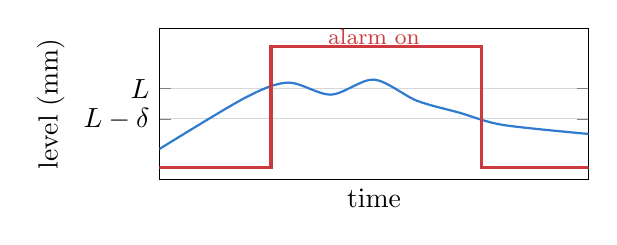
\begin{tikzpicture}
\begin{axis}[width=0.58\textwidth,height=3.5cm,xlabel={time},ylabel={level (mm)},
  xmin=0,xmax=10,ymin=470,ymax=520,ytick={490,500},yticklabels={$L-\delta$,$L$},
  xtick=\empty,grid=major,grid style={linegrey}]
\addplot[accent,thick,smooth] coordinates {(0,480)(2,497)(3,502)(4,498)(5,503)(6,496)(7,492)(8,488)(10,485)};
\addplot[badred,very thick,const plot] coordinates {(0,474)(2.6,474)(2.6,514)(7.5,514)(7.5,474)(10,474)};
\node[font=\footnotesize,badred] at (axis cs:5,517) {alarm on};
\end{axis}
\end{tikzpicture}
\caption{Hysteresis: the alarm (red) sets at $L$ and clears only below
$L-\delta$, so the wobble between 496 and 503\,mm produces a single alarm.}
\label{fig:hyst}
\end{figure}

\subsection{Timers count scans}
The minimum-flow trip uses an on-delay timer (TON): its output goes true once
its input has been true for the preset, and resets the moment the input goes
false. The timer counts \emph{scans}, not seconds. Accumulating
\code{elapsed += 0.1} reaches $0.9999999999999999$ after ten scans, and a
timer compared with \code{>=} against a 1.0\,s preset would never fire. Real
PLC timers count ticks for exactly this reason. The preset is converted once
to $\operatorname{round}(T/T_s)$ scans.

\section{Drift-free scheduling}

\code{await asyncio.sleep(period)} in a loop schedules the next wake relative
to when the previous one \emph{finished}, so every microsecond of work is
added permanently to the phase. The \code{Ticker} in \code{pyplant/clock.py}
computes absolute targets from a fixed origin instead:
\begin{equation}
  t_n = t_0 + n\,\frac{T}{\text{speed}} .
\end{equation}
Work eats into the slack, never into the phase. With a 70\,ms body on a
100\,ms period, 100 ticks land at exactly 10.000\,s rather than 17.000\,s; a
test asserts this to $10^{-12}$\,s.

\begin{figure}[htbp]
\centering
\scalebox{0.8}{%
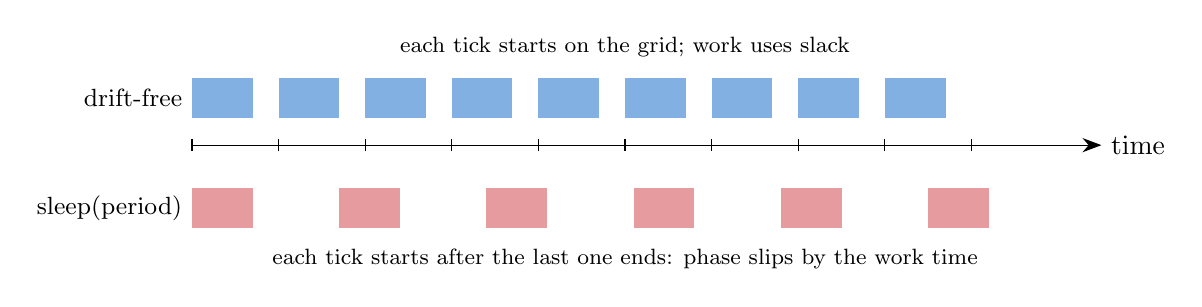
\begin{tikzpicture}[x=1.1cm,y=1cm]
  \draw[->] (0,0) -- (10.5,0) node[right]{time};
  \foreach \i in {0,...,9}{\draw (\i,0.08) -- (\i,-0.08); }
  \node[left] at (0,0.6) {\small drift-free};
  \foreach \i in {0,...,8}{\fill[accent!60] (\i,0.35) rectangle (\i+0.7,0.85);}
  \node[left] at (0,-0.8) {\small sleep(period)};
  \foreach \i in {0,...,5}{\fill[badred!50] (\i*1.7,-0.55) rectangle (\i*1.7+0.7,-1.05);}
  \node[font=\footnotesize] at (5,1.25) {each tick starts on the grid; work uses slack};
  \node[font=\footnotesize] at (5,-1.45) {each tick starts after the last one ends: phase slips by the work time};
\end{tikzpicture}}
\caption{Absolute scheduling (top) against relative sleeping (bottom) with a
70\% duty cycle.}
\label{fig:ticker}
\end{figure}

\subsection{The engine measures itself}
\tg{SCAN_MS}, \tg{SCAN_OVERRUNS} and \tg{PLC_HEARTBEAT} are real tags, trended
like any process value. The published statistics are always the previous
scan's, because this scan's duration is unknown until its write completes,
which is what real controllers do. When the engine cannot keep up, lateness
grows without bound against the fixed grid while the overrun count increments
once per scan; lateness is the signal to watch.

\section{The tag dictionary}

\code{pyplant/tags.py} is the single source of truth for every signal. Each
\code{Tag} carries a description, kind (analog or bool), owning process,
Modbus table and address, engineering unit and span, integer scale factor,
alarm limits, writability and the OPC UA area. Every other module imports its
I/O definitions from it; nothing else may hard-code an address or a scale
factor. Appendix~\ref{app:tags} lists all tags.

\subsection{Wire representation}
Analog values travel in 16-bit Modbus holding registers as
\begin{equation}
  w = \operatorname{round}(v\cdot s), \qquad
  w \in [-32768, 32767],
\end{equation}
sent as an unsigned two's-complement word. The scale $s$ is chosen per tag so
the span fits; this is checked at import. Out-of-range values are clamped,
not wrapped, so a bad value reads as a pegged instrument rather than a sign
flip. For \tg{LT101}, $s = 10$: 432.7\,mm travels as 4327 with a resolution
of 0.1\,mm. Booleans travel in coils as 0 or 1.

\subsection{Ownership and blocks}
Each tag's \code{owner} (\code{PLANT}, \code{PLC}, \code{OPER}, \code{ML})
is the only process that may write it. Addresses are grouped into declared
\emph{blocks} so a client polls a whole span in one Modbus transaction, and
import fails if a block has a gap, two blocks overlap, or a tag sits in a
block owned by another process.

\begin{theory}[No block may be written by two parties]
If one block held both the operator's setpoint and the PLC's readback, an
operator write arriving between the PLC's read and its publish would be
overwritten 100\,ms later. The faceplate is therefore split into
\code{OPER_SP}/\code{OPER_CMD} (HMI writes, PLC reads) and
\code{PLC_FACE}/\code{PLC_DIAG}/\code{PLC_ALARMS} (PLC writes, HMI reads).
\end{theory}

\section{Modbus TCP: the field layer}

\begin{figure}[htbp]
\centering
\scalebox{0.8}{%
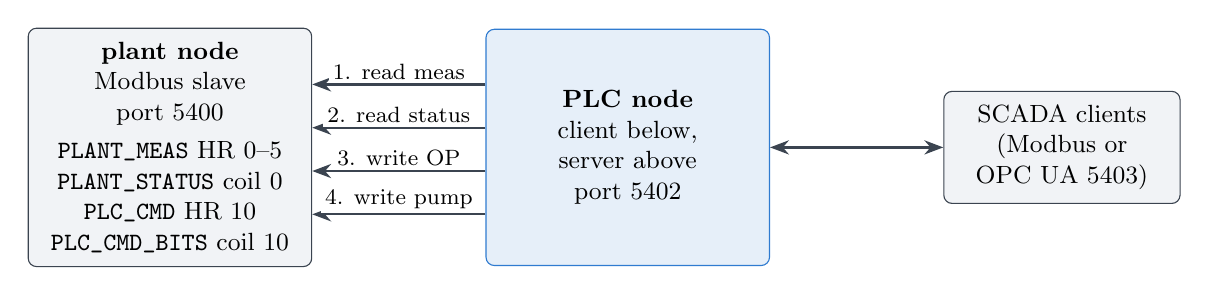
\begin{tikzpicture}[node distance=6mm and 22mm]
  \node[box,minimum width=36mm,minimum height=30mm] (plant) {\textbf{plant node}\\Modbus slave\\port 5400\\[3pt]\code{PLANT_MEAS} HR 0--5\\\code{PLANT_STATUS} coil 0\\\code{PLC_CMD} HR 10\\\code{PLC_CMD_BITS} coil 10};
  \node[hot,minimum width=36mm,minimum height=30mm,right=of plant] (plc) {\textbf{PLC node}\\client below,\\server above\\port 5402};
  \node[box,minimum width=30mm,right=of plc] (scada) {SCADA clients\\(Modbus or\\OPC UA 5403)};
  \draw[flow] ([yshift=8mm]plc.west) -- node[lbl,above]{1. read meas} ([yshift=8mm]plant.east);
  \draw[flow] ([yshift=2.5mm]plc.west) -- node[lbl,above]{2. read status} ([yshift=2.5mm]plant.east);
  \draw[flow] ([yshift=-3mm]plc.west) -- node[lbl,above]{3. write OP} ([yshift=-3mm]plant.east);
  \draw[flow] ([yshift=-8.5mm]plc.west) -- node[lbl,above]{4. write pump} ([yshift=-8.5mm]plant.east);
  \draw[flow,<->] (plc) -- (scada);
\end{tikzpicture}}
\caption{Four Modbus round trips per scan, measured at 0.7\,ms against a
100\,ms budget.}
\label{fig:modbus}
\end{figure}

The plant is a Modbus \emph{slave}, as a field device is. It has no controller,
no alarms and no memory of intent: it applies whatever is in its command
registers, so if the PLC stops writing, the valve holds its last position, as
a real one does. The PLC is both client (towards the plant) and server
(towards SCADA). It mirrors the plant measurements into its own store so the
HMI polls one address instead of two. Reads are by block, never by tag: one
\code{read_holding_registers} for six measurements is one round trip.

\section{OPC UA: the information layer}

OPC UA is the boundary between registers and meaning. Below it everything is
addresses and scale factors; above it the historian and HMI speak tag names
with units attached and never import a Modbus symbol.

The address space is generated from the tag dictionary. Each tag's
\code{area} becomes its folder path, e.g.\ \code{Plant/Unit1/LT101},
\code{PLC/LIC101/LIC101_SP} (writable) or \code{PLC/Diagnostics/SCAN_MS}.
Every analog node carries \code{EngineeringUnits} and \code{EURange} from its
declared span, so a client can scale a trend without being told anything about
the plant.

The server is a \emph{view} of the same \code{TagStore} the Modbus server
holds, not a second process image. Values are pushed outward on a refresh tick
only for nodes that changed; client writes are pushed back into the store. To
stop a refresh from reverting a fresh operator write, \code{refresh()} tracks
the last value each writable tag was seen to hold and overwrites a writable
node only when the store changed underneath it.

Clients use \emph{subscriptions}: the server pushes changes at a publishing
interval, which is why the historian is not a poller.

\chapter{SCADA: historian, HMI and alarms}
\label{ch:scada}

Supervisory control and data acquisition (SCADA) sits above the PLC. It does
not close loops; it records, displays and lets people intervene. In pyplant
the SCADA layer is three pieces: the historian collector, its query API and
the operator HMI with an ISA-18.2 alarm manager.

\section{The historian}

\subsection{Data flow}

\begin{figure}[htbp]
\centering
\scalebox{0.8}{%
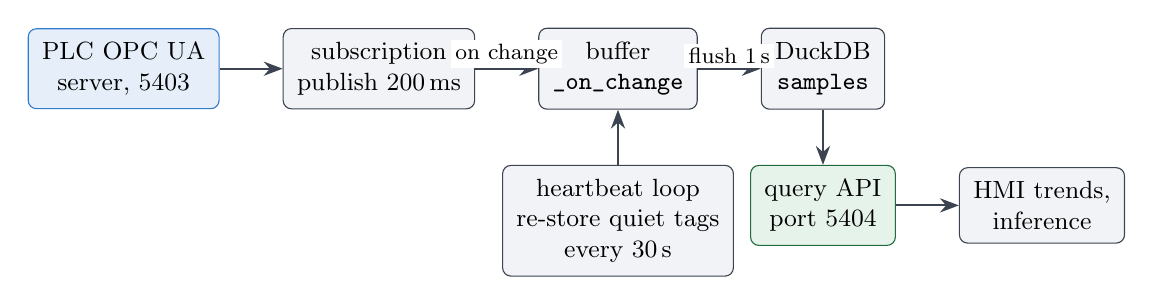
\begin{tikzpicture}[node distance=7mm and 8mm]
  \node[hot] (opc) {PLC OPC UA\\server, 5403};
  \node[box,right=of opc] (sub) {subscription\\publish 200\,ms};
  \node[box,right=of sub] (buf) {buffer\\\code{_on_change}};
  \node[box,right=of buf] (db) {DuckDB\\\code{samples}};
  \node[box,below=of buf] (hb) {heartbeat loop\\re-store quiet tags\\every 30\,s};
  \node[good,below=of db] (api) {query API\\port 5404};
  \node[box,right=of api] (cli) {HMI trends,\\inference};
  \draw[flow] (opc) -- (sub);
  \draw[flow] (sub) -- node[lbl,above]{on change} (buf);
  \draw[flow] (buf) -- node[lbl,above]{flush 1\,s} (db);
  \draw[flow] (hb) -- (buf);
  \draw[flow] (db) -- (api);
  \draw[flow] (api) -- (cli);
\end{tikzpicture}}
\caption{The historian collector (\code{pyplant/services/historian.py}).}
\label{fig:historian}
\end{figure}

The collector subscribes to every tag the PLC serves. An OPC UA subscription
already pushes only on change, which is most of what a historian's
compression does. What it does not give is an anchor for a tag that has been
quiet for an hour, so each tag is also re-stored if it has been silent for
\code{heartbeat} seconds (default 30). This is the classic exception-reporting
pair: store on change, and never let the gap exceed a maximum. Writes are
buffered and flushed in batches every second, because row-at-a-time inserts
are the usual way to make DuckDB look slow.

\subsection{Storage}
The table is in long format, one row per sample:
\begin{center}
\code{samples(ts TIMESTAMP, tag VARCHAR, value DOUBLE, quality UTINYINT)}
\end{center}
A wide table needs a migration the day a tag is added; a long table does not.
Quality is the OPC UA status flattened to \code{GOOD}~(0),
\code{UNCERTAIN}~(1) and \code{BAD}~(2). Queries ignore bad samples unless
asked.

\subsection{Resampling: last value carried forward}

Samples arrive by exception, so between two stored samples the signal did not
drift; it was \emph{held}. Linear interpolation would invent a ramp that never
existed, and on a valve position or an alarm bit that is simply wrong. The
historian builds a regular grid and uses DuckDB's \code{ASOF LEFT JOIN} to
take, for every grid instant, the last sample at or before it:
\begin{equation}
  \hat x(t_g) = x(t_j), \qquad j = \max\{\,i : t_i \le t_g\,\}.
\end{equation}
Samples stored before the window's start count too, so a window never opens
with a column of nulls just because a tag happened to be quiet.

\begin{figure}[htbp]
\centering
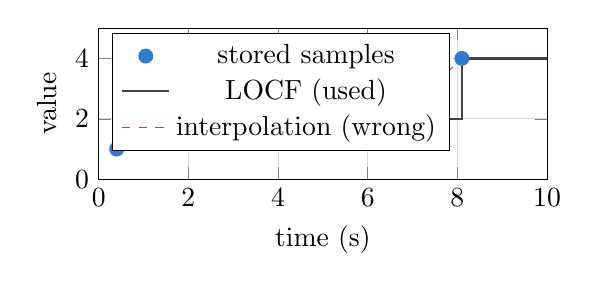
\begin{tikzpicture}
\begin{axis}[width=0.6\textwidth,height=3.5cm,xlabel={time (s)},ylabel={value},
  xmin=0,xmax=10,ymin=0,ymax=5,grid=major,grid style={linegrey},legend pos=north west]
\addplot[only marks,mark=*,accent,mark size=2.5pt] coordinates {(0.4,1)(3.2,3)(6.7,2)(8.1,4)};
\addplot[slate,thick,const plot] coordinates {(0.4,1)(3.2,1)(3.2,3)(6.7,3)(6.7,2)(8.1,2)(8.1,4)(10,4)};
\addplot[badred,dashed] coordinates {(0.4,1)(3.2,3)(6.7,2)(8.1,4)};
\legend{stored samples, LOCF (used), interpolation (wrong)}
\end{axis}
\end{tikzpicture}
\caption{Step-hold resampling against linear interpolation.}
\label{fig:locf}
\end{figure}

\subsection{Covered span}
\code{span()} is the extent of the whole database, and a window opened there
almost always starts with nulls: tags report a few milliseconds apart, so the
earliest sample belongs to exactly one of them. \code{covered_span(tags)}
returns the interval over which \emph{every} requested tag has a value, the
latest of the per-tag first samples to the latest last sample. Use it to ask
``give me everything you have''.

\begin{warn}[Wall-clock timestamps]
Timestamps are wall clock, as a real historian's are. At \code{speed} $>1$ the
recorded timeline is compressed, so a window 60 wall seconds long covers
$60\times\text{speed}$ seconds of plant time. Training data comes from the
fast runner in plant time and never touches this database.
\end{warn}

\subsection{One writer}
DuckDB takes an exclusive lock on its file, so a second process cannot open
it even to read. That is not a limitation to work around: a historian is a
service you query, not a file you share. Exactly one process writes, and
everything else asks the query API on port 5404 (Chapter~\ref{ch:api}).

\section{The operator HMI}

The HMI (\code{pyplant/hmi/app.py}; port 5405 under the workbench, 8080
when started by hand) is a FastAPI application
serving one HTML page and a JSON API. It connects to the PLC over OPC UA,
polls the faceplate every 0.5\,s, feeds the alarm manager and reads trends
from the historian API. It shows a live mimic of the two tanks, the LIC101
faceplate (SP, PV, OP, mode), pump control, trends and the alarm list.

\subsection{Write guards}
Every operator write goes through one function that rejects bad requests
before anything reaches the control system:

\begin{center}
\begin{tabular}{@{}lll@{}}
\toprule
Check & HTTP status & Example \\
\midrule
tag exists & 404 & unknown tag \\
tag is operator-writable & 403 & writing \tg{LT101} \\
analog value inside span & 422 & setpoint of 900\,mm \\
connected to the PLC & 503 & PLC is down \\
\bottomrule
\end{tabular}
\end{center}

\subsection{Pulsed reset}
\code{POST /api/reset} pulses \tg{CMD_ALM_RESET}. A latched interlock needs
an \emph{edge}, not a level: holding the reset bit true would re-clear the
latch on every scan and defeat it.

\section{Alarm management (ISA-18.2)}

A boolean that turns a row red is not alarm management. ANSI/ISA-18.2 exists
because operators need to distinguish four situations that a single ``is it
on'' flag collapses into two. pyplant implements the core state model in
\code{pyplant/hmi/alarms.py}.

\begin{figure}[htbp]
\centering
\scalebox{0.8}{%
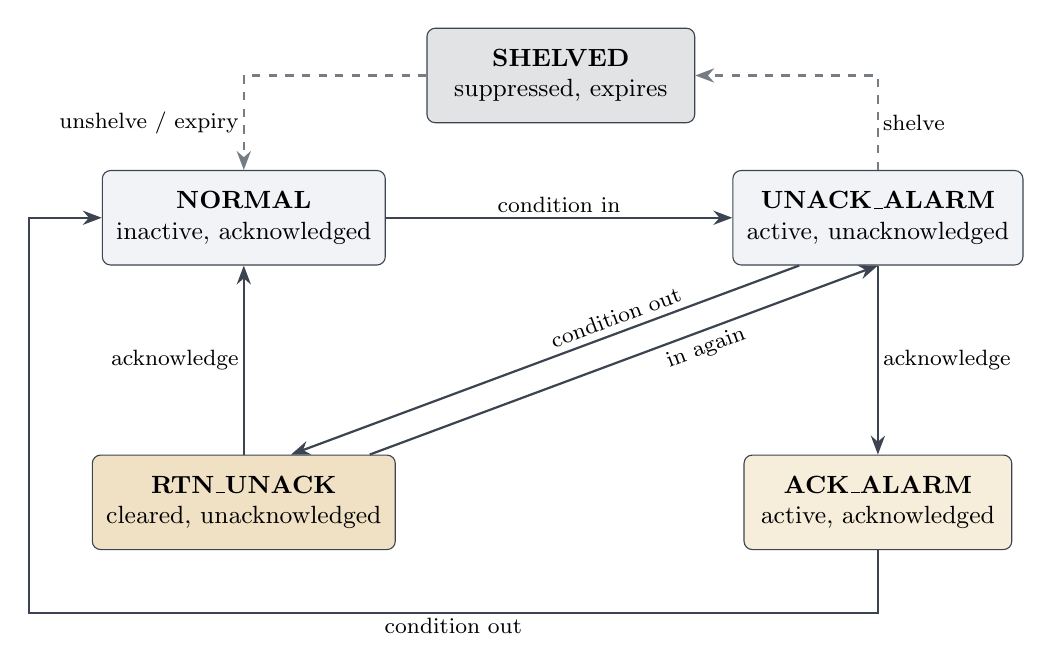
\begin{tikzpicture}[node distance=24mm and 44mm,
  st/.style={box,minimum width=34mm,minimum height=12mm}]
  \node[good,st] (n) {\textbf{NORMAL}\\inactive, acknowledged};
  \node[bad,st,right=of n] (u) {\textbf{UNACK\_ALARM}\\active, unacknowledged};
  \node[box,st,fill=warnamber!15,below=of u] (a) {\textbf{ACK\_ALARM}\\active, acknowledged};
  \node[box,st,fill=warnamber!25,below=of n] (r) {\textbf{RTN\_UNACK}\\cleared, unacknowledged};
  \node[box,st,fill=slate!15,above=12mm of $(n)!0.5!(u)$] (s) {\textbf{SHELVED}\\suppressed, expires};
  \draw[flow] (n) -- node[lbl,above]{condition in} (u);
  \draw[flow] (u) -- node[lbl,right]{acknowledge} (a);
  \draw[flow] (r) -- node[lbl,left]{acknowledge} (n);
  \draw[flow] ([xshift=-10mm]u.south) -- node[lbl,sloped,above=1pt,pos=0.35]{condition out} ([xshift=6mm]r.north);
  \draw[flow] ([xshift=16mm]r.north) -- node[lbl,sloped,below=1pt,pos=0.65]{in again} ([xshift=0mm]u.south);
  \draw[flow] (a.south) -- ++(0,-8mm) -| node[lbl,pos=0.25,below]{condition out} ([xshift=-8mm]r.west) |- (n.west);
  \draw[dflow] (s.west) -| node[lbl,pos=0.75,left]{unshelve / expiry} (n.north);
  \draw[dflow] (u.north) |- node[lbl,pos=0.25,right]{shelve} (s.east);
\end{tikzpicture}}
\caption{The ISA-18.2 alarm states implemented by \code{Alarm}. Shelving can be
entered from any state and returns to whatever the condition says at that
moment.}
\label{fig:isa}
\end{figure}

\begin{description}
  \item[NORMAL] quiet, and nobody needs to do anything.
  \item[UNACK\_ALARM] active, and nobody has looked at it yet.
  \item[ACK\_ALARM] active, and somebody has taken responsibility.
  \item[RTN\_UNACK] it cleared itself before anyone looked. This is the
        state that matters most: a transient between two operator glances
        leaves no trace in a flag-based list, and the transient nobody saw is
        often the interesting one. It stays on the list until acknowledged.
  \item[SHELVED] a deliberate, temporary, expiring silence with a reason
        recorded (default 30\,min, capped at 8\,h). The condition is still
        tracked underneath: if it goes active while shelved, the alarm comes
        back as unacknowledged on expiry.
\end{description}

\subsection{Priorities}
Priority is a design decision per alarm, not something derived from a name.
An interlock that trips the pump outranks a level approaching its limit.

\begin{center}
\begin{tabular}{@{}lll@{}}
\toprule
Alarm & Priority & Message \\
\midrule
\tg{ILK_PMP101} & CRITICAL (4) & interlock tripped, pump stopped, valve shut \\
\tg{ALM_LT101_LOLO} & HIGH (3) & tank 1 level low low \\
\tg{ALM_PT101_HIHI} & HIGH (3) & pump discharge pressure high high \\
\tg{ALM_LT101_HI} & MEDIUM (2) & tank 1 level high \\
\tg{ALM_HEALTH} & LOW (1) & model health index degraded \\
\bottomrule
\end{tabular}
\end{center}

The alarm page sorts by priority, then newest first. The summary reports the
counts per state, the number needing attention (UNACK plus RTN\_UNACK) and
the worst priority among them, which drives the banner colour.

\subsection{Operating the alarm list}
\begin{enumerate}
  \item A red row is an unacknowledged active alarm. Investigate, then press
        \ui{Ack}; it turns amber (acknowledged) and stays until the condition
        clears.
  \item A row marked \emph{returned} cleared on its own. Read it and
        acknowledge it; it then leaves the list.
  \item A chattering nuisance alarm can be shelved with a reason and a
        duration. Shelving is how you avoid operators ignoring the whole
        list instead.
  \item The interlock additionally needs \ui{Reset} once the cause is gone;
        acknowledging only clears the notification, not the trip.
\end{enumerate}

\chapter{Faults and scenarios}
\label{ch:faults}

Faults are objects applied to a running plant, never edits to the physics.
This chapter describes the fault taxonomy in \code{pyplant/faults/model.py},
the scenarios in \code{pyplant/faults/scenarios.py} that turn faults into
labelled data, and how to inject faults into the live stack.

\section{Where a fault enters}

There are three places a fault can enter the loop, and which one it uses is
the most important thing about it.

\begin{figure}[htbp]
\centering
\scalebox{0.8}{%
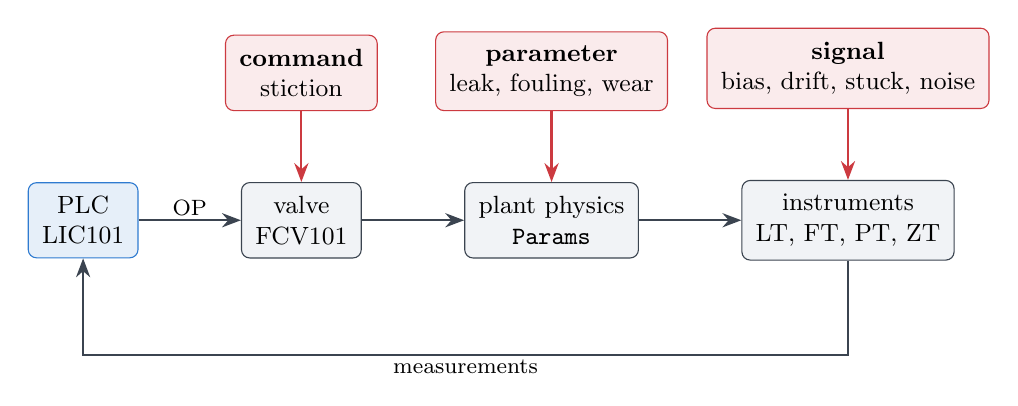
\begin{tikzpicture}[node distance=8mm and 13mm]
  \node[hot] (plc) {PLC\\LIC101};
  \node[box,right=of plc] (valve) {valve\\FCV101};
  \node[box,right=of valve] (plant) {plant physics\\\code{Params}};
  \node[box,right=of plant] (inst) {instruments\\LT, FT, PT, ZT};
  \draw[flow] (plc) -- node[lbl,above]{OP} (valve);
  \draw[flow] (valve) -- (plant);
  \draw[flow] (plant) -- (inst);
  \draw[flow] (inst.south) -- ++(0,-12mm) -| node[lbl,pos=0.25,below]{measurements} (plc.south);
  \node[bad,above=9mm of valve] (cf) {\textbf{command}\\stiction};
  \node[bad,above=9mm of plant] (pf) {\textbf{parameter}\\leak, fouling, wear};
  \node[bad,above=9mm of inst] (sf) {\textbf{signal}\\bias, drift, stuck, noise};
  \draw[flow,badred] (cf) -- (valve);
  \draw[flow,badred] (pf) -- (plant);
  \draw[flow,badred] (sf) -- (inst);
\end{tikzpicture}}
\caption{The three fault entry points, applied by \code{FaultSet.command()},
\code{FaultSet.params()} and \code{FaultSet.measure()}.}
\label{fig:faultentry}
\end{figure}

\begin{description}
  \item[Parameter faults] change the plant itself: the physics really is
        different afterwards.
  \item[Command faults] sit between the PLC and the valve: the stem does not
        do what it is told.
  \item[Signal faults] corrupt what an instrument reports while the process
        is unchanged.
\end{description}

\begin{theory}[Why the entry point matters]
A level transmitter reading 30\,mm high and a genuine 30\,mm rise produce
identical numbers in \tg{LT101}. They differ only in what the \emph{rest} of
the plant does: a real rise changes \tg{LT102} and the outflow, a bias does
not. A model that has never seen both cannot tell them apart. In a closed
loop it is worse: the controller acts on the biased reading and moves the
\emph{true} level 25\,mm down while the displayed level sits on setpoint.
\end{theory}

\section{Timing}

Every fault has a start $t_s$, an optional end $t_e$ and a ramp $T_r$. Its
strength at time $t$ is
\begin{equation}
  s(t) = \begin{cases}
   0 & t < t_s \text{ or } t \ge t_e,\\
   \min\!\big((t-t_s)/T_r,\;1\big) & T_r > 0,\\
   1 & \text{otherwise.}
  \end{cases}
\end{equation}
The ramp is not cosmetic: an abrupt leak and an incipient one over an hour are
different detection problems, and a dataset containing only step changes
trains a detector that is useless on faults that creep.

\section{The fault catalogue}

\begin{center}
\begin{tabularx}{\textwidth}{@{}lllX@{}}
\toprule
Kind & Entry & Magnitude (default) & Effect \\
\midrule
\code{leak} & parameter & \code{cda} $2\times10^{-5}$\,m$^2$ & adds a Torricelli drain on tank 1: $q_\text{leak}=C_dA\sqrt{2gh_1}$ \\
\code{fouling} & parameter & \code{loss} 0.30 & interconnect $C_dA$ multiplied by $(1-\text{loss}\cdot s)$ \\
\code{pump_wear} & parameter & \code{loss} 0.15 & pump head multiplied by $(1-\text{loss}\cdot s)$ \\
\code{stiction} & command & \code{deadband} 0.06, \code{slip} 0.04 & stem sticks inside $S$, jumps by $J$ \\
\code{sensor_bias} & signal & \code{bias} 25 (units) & reading $+\,\text{bias}\cdot s$ \\
\code{sensor_drift} & signal & \code{rate_per_min} 5 & reading $+\,\text{rate}\cdot(t-t_s)/60$ \\
\code{sensor_stuck} & signal & none & reading frozen at onset value \\
\code{sensor_noise} & signal & \code{sigma} 1.0 & reading $+\,\mathcal N(0,(\sigma s)^2)$, seeded \\
\bottomrule
\end{tabularx}
\end{center}

Signal faults take a \code{tag} (default \tg{LT101}); the corrupted value is
clamped to the tag's span, so a bias cannot read beyond the instrument's
range. Several faults can be active together; the label of a sample is the
sorted list of active fault ids joined by \code{+}, or \code{normal}.

\section{Valve stiction in detail}

Stiction is the most control-relevant fault in the set and the hardest one
for a detector fed only \tg{LT101}, because its signature lives in the phase
relationship between \tg{FCV101_OP} and \tg{ZT101}. pyplant implements the
two-parameter data-driven model (deadband $S$ plus slip jump $J$):

\begin{enumerate}
  \item While stuck, the stem position $y$ does not move.
  \item When the command $u$ moves more than $S$ away from $y$, the stem
        breaks free and lands at $u - \operatorname{sign}(u-y)(S-J)$, i.e.\
        it jumps by $J$ past the point it would have reached smoothly.
  \item While moving, the stem follows the command.
  \item On a reversal of the command direction, it sticks again.
\end{enumerate}

\begin{figure}[htbp]
\centering
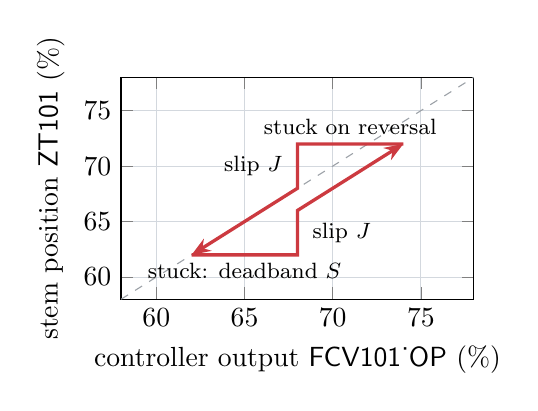
\begin{tikzpicture}
\begin{axis}[width=0.5\textwidth,height=4.4cm,xlabel={controller output \tg{FCV101_OP} (\%)},
  ylabel={stem position \tg{ZT101} (\%)},xmin=58,xmax=78,ymin=58,ymax=78,
  grid=major,grid style={linegrey},axis equal image=false]
\addplot[slate!50,dashed,domain=58:78] {x};
\addplot[badred,very thick,->] coordinates {
  (62,62)(68,62)(68,66)(74,72)};
\addplot[badred,very thick,->] coordinates {
  (74,72)(68,72)(68,68)(62,62)};
\node[font=\footnotesize] at (axis cs:65,60.6) {stuck: deadband $S$};
\node[font=\footnotesize,anchor=west] at (axis cs:68.3,64) {slip $J$};
\node[font=\footnotesize] at (axis cs:71,73.5) {stuck on reversal};
\node[font=\footnotesize,anchor=east] at (axis cs:67.7,70) {slip $J$};
\end{axis}
\end{tikzpicture}
\caption{Idealised stiction cycle in the OP--stem plane. A healthy valve lies
on the dashed diagonal; a sticky one traces a parallelogram.}
\label{fig:stiction}
\end{figure}

In a closed loop with integral action the result is a \emph{limit cycle}: the
controller keeps winding until the stem slips, the level overshoots, the
controller winds back the other way, the stem sticks on the reversal, and the
pattern repeats. The parameters are fractions of full stroke and the slip
cannot exceed the deadband.

\section{Instrument noise is not a fault}

Every scenario adds Gaussian noise to the transmitters:

\begin{center}
\begin{tabular}{@{}lccccc@{}}
\toprule
Tag & \tg{LT101} & \tg{LT102} & \tg{FT101} & \tg{PT101} & \tg{ZT101} \\
\midrule
$\sigma$ & 0.4\,mm & 0.4\,mm & 0.03\,L/min & 0.08\,kPa & 0.05\,\% \\
\bottomrule
\end{tabular}
\end{center}

It is applied as \emph{benign} \code{SensorNoise} faults: recorded, never
labelled positive. This is not decoration. A perfectly quiet loop never moves
its valve, so stiction cannot produce a limit cycle at all, and a detector
trained on noiseless signals learns a threshold that collapses the moment it
meets a real transmitter.

\section{Scenarios}

A \code{Scenario} is a reproducible run: a duration, a setpoint programme, a
fault timeline, a seed, plant parameters and a noise table. Running it
produces a trajectory in which every sample is labelled.

\begin{figure}[htbp]
\centering
\scalebox{0.8}{%
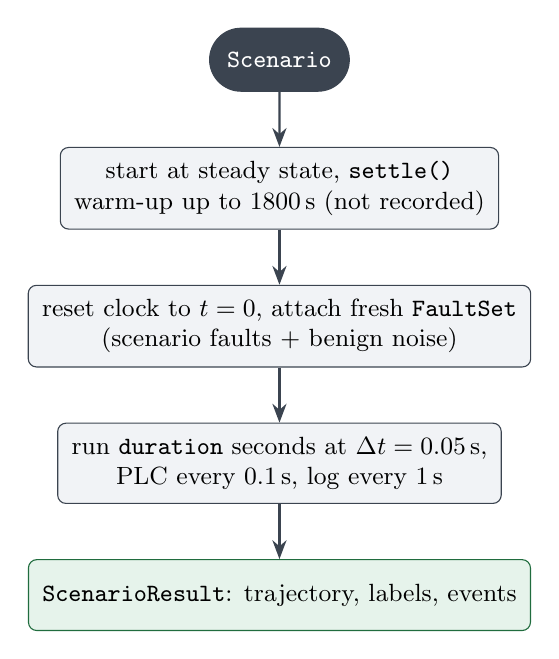
\begin{tikzpicture}[node distance=7mm]
  \node[term] (s) {\code{Scenario}};
  \node[box,below=of s] (w) {start at steady state, \code{settle()}\\warm-up up to 1800\,s (not recorded)};
  \node[box,below=of w] (r) {reset clock to $t=0$, attach fresh \code{FaultSet}\\(scenario faults + benign noise)};
  \node[box,below=of r] (run) {run \code{duration} seconds at $\Delta t=0.05$\,s,\\PLC every 0.1\,s, log every 1\,s};
  \node[good,below=of run] (out) {\code{ScenarioResult}: trajectory, labels, events};
  \draw[flow] (s) -- (w);
  \draw[flow] (w) -- (r);
  \draw[flow] (r) -- (run);
  \draw[flow] (run) -- (out);
\end{tikzpicture}}
\caption{\code{run_scenario()}. The warm-up stops a model from learning that
``faults happen at the start''.}
\label{fig:runscenario}
\end{figure}

Fault objects are stateful (stiction carries a stem position), so a fresh copy
is built for every run and the scenario's own fault list is never mutated.

\subsection{The library}
\code{library(duration)} returns one representative scenario per fault mode
plus normal operation, each with onset at 40\% of the duration and the
setpoint programme 300, 340, 280, 300\,mm at 0, 900, 1800, 2700\,s:

\begin{center}
\begin{tabular}{@{}ll@{}}
\toprule
Name & Description \\
\midrule
\code{normal} & setpoint moves only, no fault \\
\code{leak_abrupt} & tank 1 leak, step onset \\
\code{leak_incipient} & tank 1 leak opening over fifteen minutes \\
\code{pump_wear} & impeller wear 18\%, 600\,s ramp \\
\code{fouling} & interconnect restriction 35\%, 1200\,s ramp \\
\code{sensor_bias} & \tg{LT101} reads 25\,mm high \\
\code{sensor_drift} & \tg{LT101} drifting up at 1.5\,mm/min \\
\code{sensor_stuck} & \tg{LT101} frozen \\
\code{stiction} & FCV101 sticking, deadband 6\%, slip 4\% \\
\bottomrule
\end{tabular}
\end{center}

\subsection{The grid}
\code{grid(duration, magnitudes, repeats)} sweeps each fault mode across
\code{magnitudes} scale factors from 0.5 to 1.5, repeats each with different
seeds, and draws a random onset between 25\% and 60\% of the duration. It also
adds \code{repeats} normal runs. A model therefore cannot learn ``the fault
starts at 24 minutes'' instead of learning the fault. The number of scenarios
is
\begin{equation}
  N = \text{repeats}\,\big(1 + 8\times\text{magnitudes}\big),
\end{equation}
so the Standard preset (3 magnitudes, 2 repeats) builds 50 scenarios.
\code{default_dataset()} then tops the normal runs up to \code{normal_runs}
(10 for Standard), giving 58 runs in all.

\section{Injecting faults into the live stack}

The plant service exposes an injection API (Chapter~\ref{ch:api}); the
workbench \ui{Faults} tab is a form over it.

\begin{enumerate}
  \item Start the stack from \ui{Runtime} and wait for all services to be up.
  \item On \ui{Faults}, choose a kind, a magnitude, a ramp and, for sensor
        faults, a tag. Times are in plant seconds from now.
  \item Press \ui{Inject}. The fault appears in the active list with its id.
  \item Watch the HMI: the PV may not move at all (integral action), but the
        OP and the health index will.
  \item Clear one fault or all of them. \code{GET /api/truth} always returns
        the true state, including what the instruments do not show.
\end{enumerate}

From Python:
\begin{lstlisting}
from pyplant.faults.model import Leak
from pyplant.faults.scenarios import Scenario, run_scenario
sc = Scenario("my_leak", duration=1800,
              faults=[Leak("leak", t_start=600, cda=3e-5, ramp=300)])
res = run_scenario(sc)
df = res.frame()        # time series + label + faulty columns
print(res.events)       # ground truth
\end{lstlisting}

\chapter{Machine learning for fault detection}
\label{ch:ml}

This chapter covers the data-driven diagnosis pipeline in \code{pyplant/ml}:
how runs become feature windows, the theory behind each classical detector,
how thresholds and the health index are set, and how a detection is traced
back to an instrument. The neural detector is in Chapter~\ref{ch:dl} and the
evaluation method in Chapter~\ref{ch:eval}.

\section{The pipeline}

\begin{figure}[htbp]
\centering
\scalebox{0.8}{%
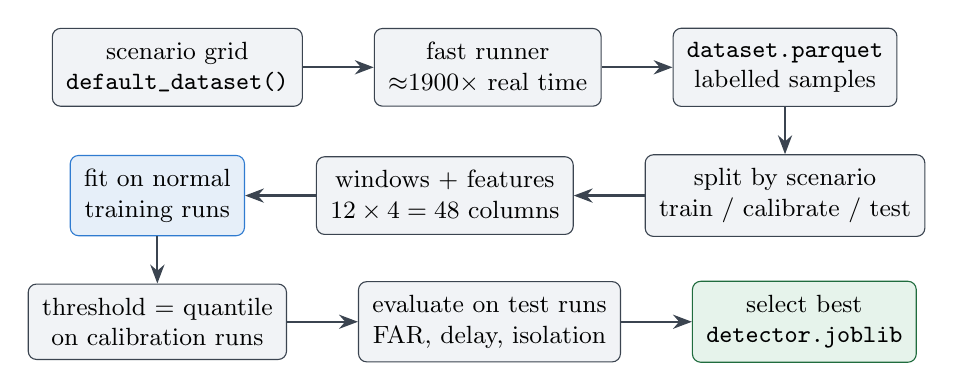
\begin{tikzpicture}[node distance=6mm and 9mm]
  \node[box] (grid) {scenario grid\\\code{default_dataset()}};
  \node[box,right=of grid] (sim) {fast runner\\$\approx$1900$\times$ real time};
  \node[box,right=of sim] (pq) {\code{dataset.parquet}\\labelled samples};
  \node[box,below=of pq] (split) {split by scenario\\train / calibrate / test};
  \node[box,left=of split] (win) {windows + features\\$12\times4=48$ columns};
  \node[hot,left=of win] (fit) {fit on normal\\training runs};
  \node[box,below=of fit] (cal) {threshold = quantile\\on calibration runs};
  \node[box,right=of cal] (ev) {evaluate on test runs\\FAR, delay, isolation};
  \node[good,right=of ev] (sel) {select best\\\code{detector.joblib}};
  \draw[flow] (grid) -- (sim);
  \draw[flow] (sim) -- (pq);
  \draw[flow] (pq) -- (split);
  \draw[flow] (split) -- (win);
  \draw[flow] (win) -- (fit);
  \draw[flow] (fit) -- (cal);
  \draw[flow] (cal) -- (ev);
  \draw[flow] (ev) -- (sel);
\end{tikzpicture}}
\caption{From simulation to a deployable detector. The workbench \ui{Data}
and \ui{Model} tabs run exactly these steps.}
\label{fig:mlpipe}
\end{figure}

\section{Why unsupervised, trained on normal only}

The detectors never see a fault during training. This is not a purity
exercise: a real plant has years of normal operation and a handful of
documented failures, so a supervised classifier would be trained on the rarest
thing it will ever meet and could not recognise a mode nobody labelled.
Instead each detector learns what \emph{normal} looks like and scores how far
a window departs from it. Fault data is used only to measure the result.

Formally, given normal feature vectors $\{\bm x_i\}$ drawn from $p_0$, each
detector defines an anomaly score $a(\bm x)$ that is small where $p_0$ is
dense and large where it is not. A window is flagged when $a(\bm x) > \theta$.

\section{Windows}

A detector looks at a window, not a sample, because what distinguishes faults
are shapes over time: a leak shifts a level, a drift tilts it, stiction makes
it oscillate. One sample cannot express any of those.

\begin{figure}[htbp]
\centering
\scalebox{0.8}{%
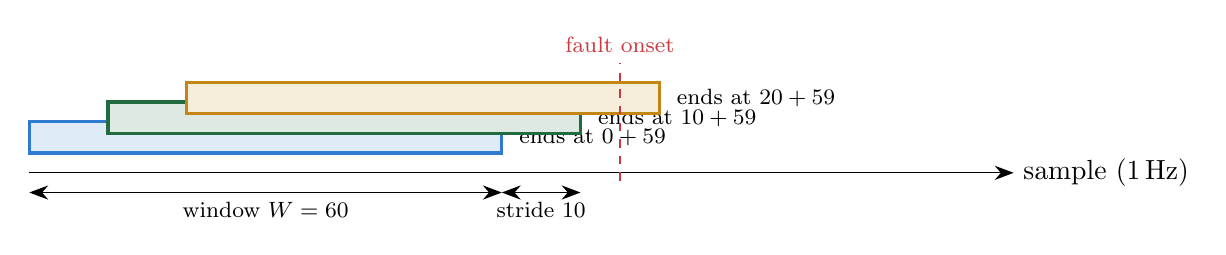
\begin{tikzpicture}[x=0.1cm,y=1cm]
  \draw[->] (0,0) -- (125,0) node[right]{sample (1\,Hz)};
  \foreach \s/\c in {0/accent,10/okgreen!70!black,20/warnamber}{
    \draw[\c,very thick,fill=\c!15] (\s,{0.25+\s/40}) rectangle (\s+60,{0.65+\s/40});
    \node[font=\footnotesize,anchor=west] at (\s+61,{0.45+\s/40}) {ends at $\s+59$};
  }
  \draw[<->] (0,-0.25) -- node[below,font=\footnotesize]{window $W=60$} (60,-0.25);
  \draw[<->] (60,-0.25) -- node[below,font=\footnotesize]{stride 10} (70,-0.25);
  \draw[badred,dashed,thick] (75,-0.1) -- (75,1.4) node[above,font=\footnotesize]{fault onset};
\end{tikzpicture}}
\caption{Overlapping windows. Each is labelled by its \emph{last} sample, so a
window straddling the onset is not counted as faulty from its first sample.}
\label{fig:windows}
\end{figure}

Defaults: \code{WINDOW = 60} samples (one minute) and \code{STRIDE = 10}. A
window labelled by its first sample would make detection delay look negative.

\section{Features}

\subsection{Channels}
Nine measured or controller tags are used:
\tg{LT101}, \tg{LT102}, \tg{FT101}, \tg{FT102}, \tg{PT101}, \tg{ZT101},
\tg{FCV101_OP}, \tg{LIC101_SP} and \tg{LIC101_ERR}. Controller output is
included deliberately: in a closed loop the controller absorbs the fault, so
the PV alone hides it (Section~\ref{sec:masking}).

Three more channels are computed from first principles, each because the
fault shows up in a difference that no single tag contains:
\begin{align}
  \text{OP\_MINUS\_ZT} &= \text{FCV101\_OP} - \text{ZT101}, \\
  \text{FLOW\_IMBALANCE} &= \text{FT101} - \text{FT102}, \\
  \text{HEAD\_RESIDUAL} &= \text{PT101} - \frac{\Delta p_0}{1000}
     \Big(1-\big(\tfrac{q}{q_\text{max}}\big)^2\Big),
\end{align}
where $q$ is \tg{FT101} in m$^3$/s.
\tg{OP_MINUS_ZT} is zero on a healthy valve, and a sticking one opens a gap.
\tg{FLOW_IMBALANCE} is zero at steady state by conservation of mass, and a
leak makes it positive: a conservation law, not a learned correlation.
\tg{HEAD_RESIDUAL} is the pump pressure minus what the pump curve says it
should develop at the delivered flow, and impeller wear opens it.
Giving a model the residual of a physical relationship is cheaper and more
robust than making it learn the relationship.

\subsection{Statistics}
Each of the $12$ channels is reduced to four numbers over the window,
$\{\textit{last}, \textit{mean}, \textit{std}, \textit{slope}\}$, giving $48$
features. The slope is the least-squares slope in units per sample,
\begin{equation}
  \beta = \frac{\sum_k (k-\bar k)(x_k - \bar x)}{\sum_k (k-\bar k)^2}.
\end{equation}

\begin{center}
\begin{tabular}{@{}lll@{}}
\toprule
Statistic & Meaning & Where faults show \\
\midrule
last & where it is now & bias, stuck \\
mean & where it has been & leak, fouling, wear \\
std & how much it is moving & stiction (limit cycle), stuck (std $\to$ 0) \\
slope & which way it is going & drift, incipient faults \\
\bottomrule
\end{tabular}
\end{center}

Sixty samples of twelve channels would be 720 nearly redundant numbers. Four
statistics per channel is small enough to train on a modest dataset and keeps
every feature attributable to one channel, which is what makes isolation
possible. Features are named \code{CHANNEL::stat}, e.g.\
\code{FLOW_IMBALANCE::mean}.

\subsection{Standardisation}
Every detector first standardises with statistics of the normal training set:
\begin{equation}
  z_j = \frac{x_j - \mu_j}{\sigma_j}.
\end{equation}
In these units ``normal'' is centred at the origin with unit spread in every
direction, and all scores below are computed on $\bm z$.

\section{Detector 1: z-score limits}

The most straightforward method there is: no model at all. The reconstruction
is the normal mean, which is zero in standardised units, so the score is
\begin{equation}
  a_\text{z}(\bm x) = \sum_{j=1}^{48} z_j^2 .
\end{equation}

\begin{theory}[Interpretation]
If the features were independent Gaussians, $a_\text{z}$ would follow a
$\chi^2$ distribution with 48 degrees of freedom and a fixed limit would set a
known false alarm rate. They are not independent (\tg{LT101} and
\tg{LIC101_ERR} are nearly the same signal), which is why the threshold is
taken empirically from calibration data instead. The z-score is the baseline
every other method must beat; if it cannot be beaten, the honest report says
so.
\end{theory}

\section{Detector 2: PCA and the SPE statistic}

Principal component analysis is the basis of classical multivariate
statistical process control (MSPC). Normal operation of a plant governed by a
few physical relationships occupies a low-dimensional subspace of feature
space; a fault that breaks a relationship pushes data \emph{off} that
subspace.

\subsection{Theory}
With the standardised training matrix $Z\in\mathbb R^{n\times m}$, the
covariance $S = Z^\top Z/(n-1)$ has the eigendecomposition $S = P\Lambda
P^\top$ with eigenvalues $\lambda_1\ge\lambda_2\ge\dots$. Keep the first $k$
eigenvectors $P_k$, chosen as the smallest $k$ that explains 95\% of the
variance:
\begin{equation}
  \frac{\sum_{i\le k}\lambda_i}{\sum_i \lambda_i} \ge 0.95 .
\end{equation}
A window is projected onto the subspace and back, $\hat{\bm z} = P_kP_k^\top
\bm z$, and the score is the \emph{squared prediction error} (SPE, the $Q$
statistic):
\begin{equation}
  a_\text{PCA}(\bm x) = \text{SPE} = \lVert \bm z - \hat{\bm z} \rVert^2
  = \lVert (I - P_kP_k^\top)\,\bm z \rVert^2 .
\end{equation}

\begin{figure}[htbp]
\centering
\scalebox{0.8}{%
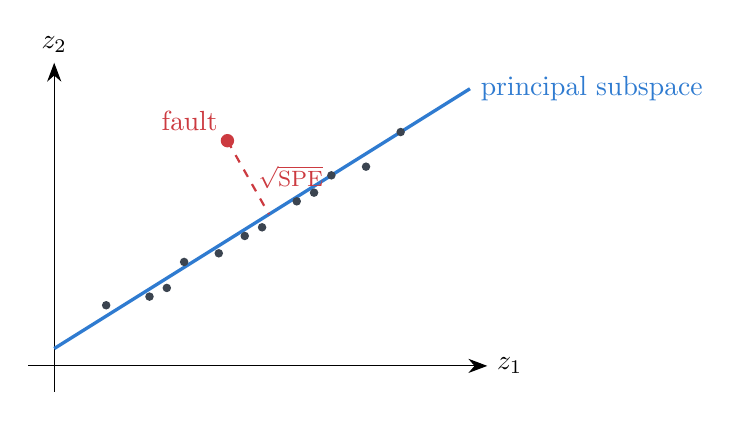
\begin{tikzpicture}[scale=1.1]
  \draw[->] (-0.3,0) -- (5,0) node[right]{$z_1$};
  \draw[->] (0,-0.3) -- (0,3.5) node[above]{$z_2$};
  \draw[accent,very thick] (0,0.2) -- (4.8,3.2) node[right]{principal subspace};
  \foreach \x/\y in {0.6/0.7,1.1/0.8,1.5/1.2,1.9/1.3,2.4/1.6,2.8/1.9,3.2/2.2,3.6/2.3,4.0/2.7,1.3/0.9,2.2/1.5,3.0/2.0}
    \fill[slate] (\x,\y) circle (1.4pt);
  \fill[badred] (2.0,2.6) circle (2.2pt) node[above left]{fault};
  \draw[badred,thick,dashed] (2.0,2.6) -- (2.48,1.75) node[midway,right,font=\footnotesize]{$\sqrt{\text{SPE}}$};
\end{tikzpicture}}
\caption{Normal data (grey) lies near the principal subspace. A fault that
breaks the correlation is far from it even when each coordinate is within its
normal range.}
\label{fig:pca}
\end{figure}

The second classical statistic, Hotelling's $T^2 = \bm z^\top P_k
\Lambda_k^{-1} P_k^\top \bm z$, measures unusual variation \emph{within} the
subspace. pyplant uses SPE only, because the faults of interest break
correlations rather than scale them.

\section{Detector 3: isolation forest}

An isolation forest does not model density or reconstruct anything. It exploits
the observation that anomalies are \emph{few and different}, so random
partitioning isolates them in fewer splits than normal points.

\subsection{Theory}
Each of the $t = 200$ trees is built on a random subsample of size $\psi$ by
repeatedly choosing a random feature and a random split value between its
minimum and maximum, until every point is alone. The path length $h(\bm x)$
is the number of splits needed to isolate $\bm x$. Averaged over trees and
normalised by the expected path length of an unsuccessful search in a binary
search tree,
\begin{equation}
  c(\psi) = 2H(\psi-1) - \frac{2(\psi-1)}{\psi}, \qquad
  H(i) \approx \ln i + 0.5772,
\end{equation}
the anomaly score is
\begin{equation}
  a_\text{IF}(\bm x) = 2^{-\mathbb E[h(\bm x)] / c(\psi)} \in (0, 1] .
\end{equation}
Scores near 1 are anomalies, scores well below 0.5 are normal. The code uses
the negated \code{score_samples} of scikit-learn, which is exactly this
quantity, so larger is worse and the threshold and health index work
unchanged.

\begin{figure}[htbp]
\centering
\scalebox{0.8}{%
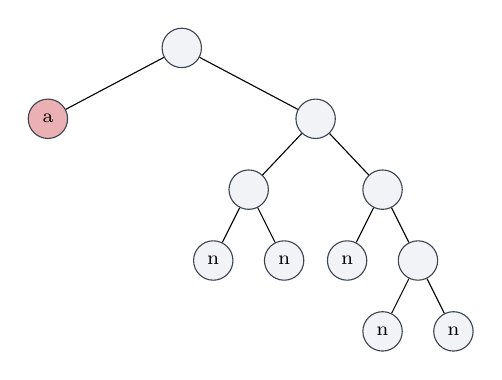
\begin{tikzpicture}[level distance=9mm,
  level 1/.style={sibling distance=34mm},
  level 2/.style={sibling distance=17mm},
  level 3/.style={sibling distance=9mm},
  every node/.style={circle,draw=slate,fill=panelgrey,minimum size=5mm,inner sep=0pt,font=\scriptsize}]
  \node {}
    child {node[fill=badred!40] {a}}
    child {node {}
      child {node {}
        child {node {n}} child {node {n}}}
      child {node {}
        child {node {n}} child {node {}
          child {node {n}} child {node {n}}}}};
\end{tikzpicture}}
\caption{One isolation tree. The anomaly \textsf{a} is isolated after one
split; normal points \textsf{n} need three or four.}
\label{fig:iforest}
\end{figure}

Because it has no reconstruction, the isolation forest's contributions fall
back to the standardised deviations $z_j^2$ (the same as the z-score
detector).

\section{Thresholds}

Every detector's threshold is a quantile of its score on \emph{held-out
normal} data:
\begin{equation}
  \theta = Q_{q}\big(\{a(\bm x_i) : \bm x_i \in \text{calibration runs}\}\big),
  \qquad q = 0.995 .
\end{equation}
Setting it on the training set measures how well the model memorised, not
how often it will cry wolf. With $q=0.995$, about one normal window in 200
is above threshold; the persistence rule of Chapter~\ref{ch:eval} turns that
into near-zero false alarms.

\section{The health index}

Raw scores have no stable scale: retrain the model and they change entirely.
The health index maps any score onto $0$--$100$ with the threshold pinned at
50 and one decade of score per 50 points:
\begin{equation}
  \text{HI} = \operatorname{clip}\!\Big(50\log_{10}\frac{a}{\theta} + 50,\;0,\;100\Big).
\end{equation}

\begin{figure}[htbp]
\centering
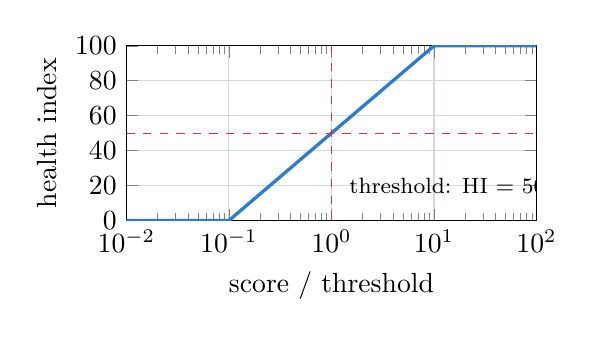
\begin{tikzpicture}
\begin{axis}[width=0.56\textwidth,height=3.8cm,xmode=log,xlabel={score / threshold},
  ylabel={health index},xmin=0.01,xmax=100,ymin=0,ymax=100,grid=major,
  grid style={linegrey}]
\addplot[accent,very thick,domain=0.01:100,samples=200]{min(max(50*log10(x)+50,0),100)};
\addplot[badred,dashed] coordinates {(1,0)(1,100)};
\addplot[badred,dashed] coordinates {(0.01,50)(100,50)};
\node[font=\footnotesize,anchor=west] at (axis cs:1.2,20) {threshold: HI = 50};
\end{axis}
\end{tikzpicture}
\caption{Health index against normalised score. A badly broken plant
(10$\times$ threshold, HI 100) stays distinguishable from a marginal one
(HI just above 50).}
\label{fig:health}
\end{figure}

Pinning the threshold to 50 is what lets an alarm limit on the
\tg{HEALTH_INDEX} tag stay where the alarm engineer put it across a retrain.

\begin{note}[Online inference]
The tag dictionary reserves an \code{ML_RESULT} block (\tg{HEALTH_INDEX},
\tg{TOP_CONTRIB}, \tg{ML_HEARTBEAT}) and the \tg{ALM_HEALTH} alarm for an
inference service that writes the health index back into the control
system. This release computes scores, health index and contributions in
Python and in the workbench \ui{Model} tab; no service writes those tags
yet. Chapter~\ref{ch:extend} sketches how to add one.
\end{note}

\section{Isolation: contributions}

Detection says \emph{that} something is wrong; isolation says \emph{where}.
The reconstruction-based detectors produce a per-feature residual
$\bm r = \bm z - \hat{\bm z}$. Every feature belongs to one channel, so summing
squared residuals by channel and normalising gives each channel's share of the
anomaly:
\begin{equation}
  c_k = \frac{\sum_{j \in \text{channel }k} r_j^2}{\sum_j r_j^2},
  \qquad \sum_k c_k = 1 .
\end{equation}
The \emph{top channel} is $\arg\max_k c_k$. This is the same argument
classical contribution plots rest on. Expected top channels for a fully
developed fault:

\begin{center}
\begin{tabular}{@{}ll@{}}
\toprule
Fault & Expected top channel \\
\midrule
leak & \tg{FLOW_IMBALANCE} \\
pump wear & \tg{HEAD_RESIDUAL} \\
stiction & \tg{OP_MINUS_ZT} \\
fouling & \tg{LT102} or \tg{FT102} \\
sensor faults & not scored (see Chapter~\ref{ch:eval}) \\
\bottomrule
\end{tabular}
\end{center}

\section{Using the detectors from Python}

\begin{lstlisting}
from pyplant.ml.dataset import load, split_scenarios, windowed
from pyplant.ml.detector import make_detector
from pyplant.ml.features import WindowSpec

frame = load("work/demo/dataset.parquet")
data  = windowed(frame, WindowSpec(window=60, stride=10))
split = split_scenarios(frame, seed=0)

det = make_detector("pca", quantile=0.995)     # zscore | pca | isolation_forest | autoencoder
det.fit(data.of_scenarios(split.train).X, data.names)
det.calibrate(data.of_scenarios(split.calibrate).X)

test = data.of_scenarios(split.test_faulty)
hi   = det.health(test.X)          # 0-100, 50 = threshold
top  = det.top_channel(test.X)     # e.g. 'FLOW_IMBALANCE'
det.save("my_detector.joblib")
\end{lstlisting}

\chapter{Deep learning: the autoencoder detector}
\label{ch:dl}

PCA finds the best \emph{linear} subspace for normal data. The plant is not
linear: Torricelli drains go as $\sqrt h$, the pump curve is quadratic and the
valve is equal-percentage. An autoencoder learns a \emph{non-linear} manifold
with the same scoring and the same contribution analysis. This chapter
explains the neural-network theory behind it and how it is trained here.

\section{Neural network fundamentals}

\subsection{The neuron and the layer}
A layer maps an input vector $\bm h^{(l-1)}$ to
\begin{equation}
  \bm h^{(l)} = \phi\big(W^{(l)}\bm h^{(l-1)} + \bm b^{(l)}\big),
\end{equation}
with weights $W^{(l)}$, biases $\bm b^{(l)}$ and an element-wise non-linear
activation $\phi$. Stacking layers gives a multilayer perceptron (MLP), which
by the universal approximation theorem can represent any continuous function
on a compact set given enough units.

\subsection{Activation}
pyplant uses the hyperbolic tangent,
\begin{equation}
  \tanh(a) = \frac{e^a - e^{-a}}{e^a + e^{-a}}, \qquad
  \tanh'(a) = 1 - \tanh^2(a).
\end{equation}
It is smooth, zero-centred (which suits standardised inputs) and saturates
gently. The output layer is linear, because standardised features are not
bounded.

\subsection{Learning: loss, backpropagation and Adam}
Training minimises the mean squared error over a batch $\mathcal B$,
\begin{equation}
  \mathcal L(\Theta) = \frac{1}{|\mathcal B|}\sum_{i\in\mathcal B}
  \lVert \bm z_i - f_\Theta(\bm z_i)\rVert^2 + \alpha\lVert\Theta\rVert^2 ,
\end{equation}
where the second term is a small L2 weight penalty ($\alpha = 10^{-4}$, the
scikit-learn default). Gradients $\nabla_\Theta\mathcal L$ are computed by
backpropagation, the chain rule applied layer by layer from the output back
to the input. Parameters are updated with Adam, which keeps running averages
of the gradient and its square:
\begin{align}
  \bm m_t &= \beta_1 \bm m_{t-1} + (1-\beta_1)\bm g_t, &
  \bm v_t &= \beta_2 \bm v_{t-1} + (1-\beta_2)\bm g_t^2, \\
  \Theta_t &= \Theta_{t-1} - \eta\,\frac{\hat{\bm m}_t}{\sqrt{\hat{\bm v}_t}+\epsilon},
  & \hat{\bm m}_t &= \frac{\bm m_t}{1-\beta_1^t},\;
    \hat{\bm v}_t = \frac{\bm v_t}{1-\beta_2^t},
\end{align}
with learning rate $\eta = 10^{-3}$, $\beta_1=0.9$, $\beta_2=0.999$.

\subsection{Generalisation and early stopping}
A network with enough capacity can memorise its training set, in which case it
reconstructs \emph{everything} well, faults included, and becomes useless as a
detector. 15\% of the training windows are held back as a validation set, and
training stops when the validation loss has not improved for 25 epochs
(\emph{early stopping}), up to a maximum of 1500 iterations.

\section{The autoencoder}

An autoencoder is a network trained to reproduce its own input through a
narrow \emph{bottleneck}. The encoder compresses the 48 standardised features
to 8 numbers; the decoder expands them back. Because the bottleneck is
narrower than the input, the network can reproduce only inputs that resemble
what it was trained on: it learns the manifold of normal operation.

\begin{figure}[htbp]
\centering
\scalebox{0.8}{%
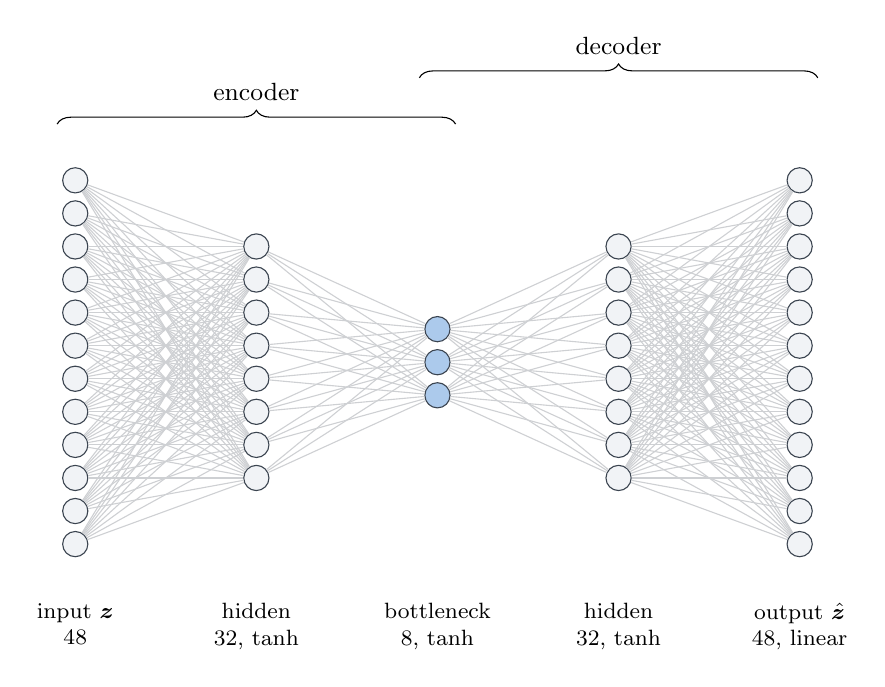
\begin{tikzpicture}[x=2.3cm,y=0.42cm,
  n/.style={circle,draw=slate,fill=panelgrey,minimum size=3.2mm,inner sep=0pt},
  b/.style={n,fill=accent!40}]
  \foreach \l/\k/\style in {0/12/n,1/8/n,2/3/b,3/8/n,4/12/n}{
    \foreach \i in {1,...,\k}{
      \node[\style] (L\l-\i) at (\l,{\i-(\k+1)/2}) {};
    }
  }
  \foreach \a/\ka/\b/\kb in {0/12/1/8,1/8/2/3,2/3/3/8,3/8/4/12}{
    \foreach \i in {1,...,\ka}{\foreach \j in {1,...,\kb}{
      \draw[slate!25] (L\a-\i) -- (L\b-\j);}}
  }
  \node[below,font=\footnotesize,align=center] at (0,-7) {input $\bm z$\\48};
  \node[below,font=\footnotesize,align=center] at (1,-7) {hidden\\32, tanh};
  \node[below,font=\footnotesize,align=center] at (2,-7) {bottleneck\\8, tanh};
  \node[below,font=\footnotesize,align=center] at (3,-7) {hidden\\32, tanh};
  \node[below,font=\footnotesize,align=center] at (4,-7) {output $\hat{\bm z}$\\48, linear};
  \draw[decorate,decoration={brace,amplitude=5pt}] (-0.1,7.2) -- node[above=5pt,font=\small]{encoder} (2.1,7.2);
  \draw[decorate,decoration={brace,amplitude=5pt}] (1.9,8.6) -- node[above=5pt,font=\small]{decoder} (4.1,8.6);
\end{tikzpicture}}
\caption{The 48--32--8--32--48 autoencoder (drawn with fewer units). It is
trained to output its input.}
\label{fig:ae}
\end{figure}

\begin{center}
\begin{tabular}{@{}lll@{}}
\toprule
Setting & Value & Field in \code{AutoencoderDetector} \\
\midrule
hidden layers & (32, 8, 32) & \code{hidden} \\
activation & tanh & fixed \\
optimiser & Adam, $\eta = 10^{-3}$ & fixed \\
maximum iterations & 1500 & \code{max_iter} \\
early stopping & 15\% validation, patience 25 & fixed \\
random seed & 0 & \code{seed} \\
\bottomrule
\end{tabular}
\end{center}

\subsection{Relationship to PCA}
A linear autoencoder (identity activations) trained with MSE learns exactly
the principal subspace: its optimum spans the same space as the top $k$
principal components. PCA is therefore the linear special case, and the
autoencoder earns its place only if the non-linearity buys detection that PCA
misses. That is why both are trained and the comparison is kept on record.

\section{Scoring, threshold and isolation}

The autoencoder uses the same machinery as PCA:
\begin{equation}
  a_\text{AE}(\bm x) = \lVert \bm z - f_\Theta(\bm z) \rVert^2,
\end{equation}
the same calibration quantile, the same health index and the same
per-channel contributions of the residual (Chapter~\ref{ch:ml}). Only the
reconstruction changes.

\begin{figure}[htbp]
\centering
\scalebox{0.8}{%
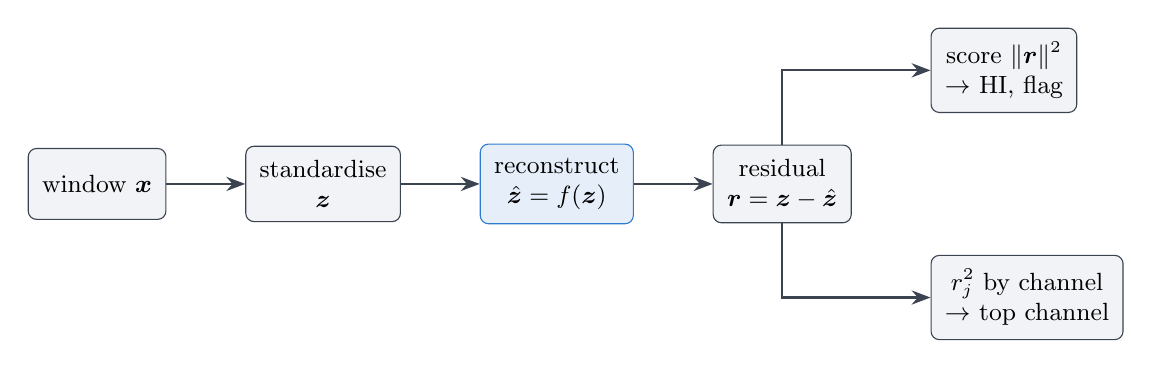
\begin{tikzpicture}[node distance=7mm and 10mm]
  \node[box] (x) {window $\bm x$};
  \node[box,right=of x] (z) {standardise\\$\bm z$};
  \node[hot,right=of z] (f) {reconstruct\\$\hat{\bm z}=f(\bm z)$};
  \node[box,right=of f] (r) {residual\\$\bm r=\bm z-\hat{\bm z}$};
  \node[box,above right=4mm and 10mm of r] (s) {score $\lVert\bm r\rVert^2$\\$\to$ HI, flag};
  \node[box,below right=4mm and 10mm of r] (c) {$r_j^2$ by channel\\$\to$ top channel};
  \draw[flow] (x) -- (z);
  \draw[flow] (z) -- (f);
  \draw[flow] (f) -- (r);
  \draw[flow] (r) |- (s);
  \draw[flow] (r) |- (c);
\end{tikzpicture}}
\caption{One scoring pass, identical for PCA and the autoencoder.}
\label{fig:aescore}
\end{figure}

\section{Practical advice}

\begin{itemize}
  \item \textbf{More data before more layers.} With the Quick preset there are
        only a few normal runs; a bigger network will memorise them. Use the
        Standard or Thorough preset before changing \code{hidden}.
  \item \textbf{Bottleneck width} controls the trade-off: too wide and faults
        reconstruct well (missed detections), too narrow and normal variation
        does not (false alarms). 8 is a good starting point for 48 features.
  \item \textbf{Seeds matter.} Training is stochastic. Compare methods over
        two or three seeds before concluding one is better.
  \item \textbf{Check against PCA.} If the autoencoder does not beat PCA on
        detection rate and false alarms, deploy PCA. The selection rule does
        this automatically.
\end{itemize}

To change the architecture:
\begin{lstlisting}
from pyplant.ml.detector import AutoencoderDetector
det = AutoencoderDetector(quantile=0.995, hidden=(64, 16, 64), max_iter=3000, seed=1)
\end{lstlisting}

\chapter{Evaluating and selecting a detector}
\label{ch:eval}

A detector's numbers mean nothing unless the data split is honest and the
metrics are the ones an operator would recognise. This chapter describes the
split in \code{pyplant/ml/dataset.py}, the metrics in
\code{pyplant/ml/evaluate.py}, and the rule that picks the detector to
deploy.

\section{Split by scenario, never by sample}

Windows overlap, and neighbouring windows from one run are nearly identical. A
random sample split puts window 41 in training and window 42 in test; the
model scores brilliantly on data it has effectively already seen, and the
number is not slightly optimistic, it is meaningless. Whole runs are split
instead.

\begin{figure}[htbp]
\centering
\scalebox{0.8}{%
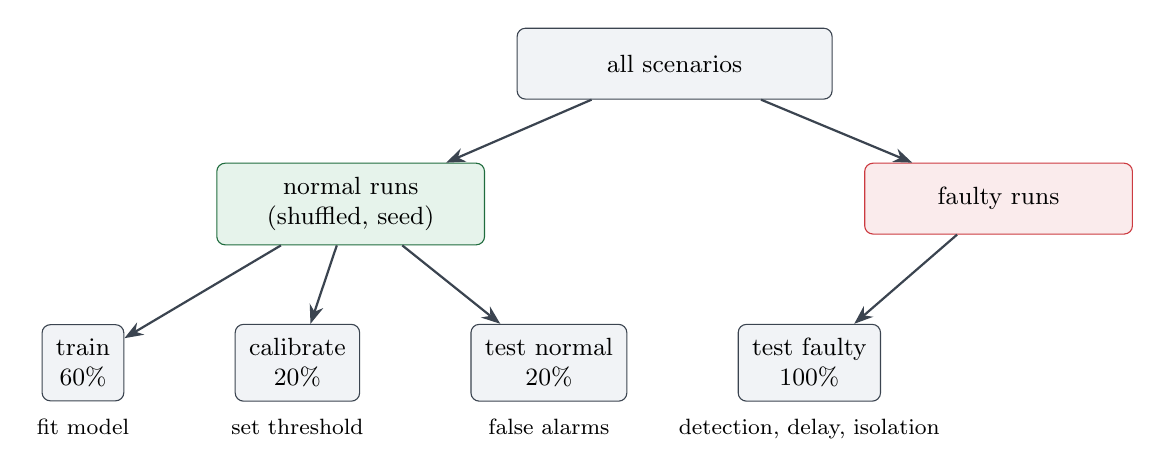
\begin{tikzpicture}[node distance=5mm and 14mm]
  \node[box,minimum width=40mm] (all) {all scenarios};
  \node[good,below left=8mm and 4mm of all,minimum width=34mm] (nor) {normal runs\\(shuffled, seed)};
  \node[bad,below right=8mm and 4mm of all,minimum width=34mm] (fau) {faulty runs};
  \node[box,below=10mm of nor,xshift=-34mm] (tr) {train\\60\%};
  \node[box,right=of tr] (ca) {calibrate\\20\%};
  \node[box,right=of ca] (tn) {test normal\\20\%};
  \node[box,right=of tn] (tf) {test faulty\\100\%};
  \draw[flow] (all) -- (nor);
  \draw[flow] (all) -- (fau);
  \draw[flow] (nor) -- (tr);
  \draw[flow] (nor) -- (ca);
  \draw[flow] (nor) -- (tn);
  \draw[flow] (fau) -- (tf);
  \node[below=1mm of tr,font=\footnotesize] {fit model};
  \node[below=1mm of ca,font=\footnotesize] {set threshold};
  \node[below=1mm of tn,font=\footnotesize] {false alarms};
  \node[below=1mm of tf,font=\footnotesize] {detection, delay, isolation};
\end{tikzpicture}}
\caption{\code{split_scenarios()}. Normal runs are divided three ways; faulty
runs are used only for testing.}
\label{fig:split}
\end{figure}

Each pool has a single job. Using one pool for fitting, thresholding and false
alarm measurement flatters the threshold. At least three normal runs are
required; the Quick preset makes six and the Standard preset ten. Because each
grid entry has its own seed, magnitude and onset, held-out runs differ from
training runs in the ways that matter operationally.

\section{Persistence}

A single flagged window is not a detection. A detection is declared at the
first window of the first run of $p = 3$ consecutive flagged windows
(\code{PERSISTENCE}). With a 10\,s stride this costs at most 20\,s of delay.

\begin{figure}[htbp]
\centering
\scalebox{0.8}{%
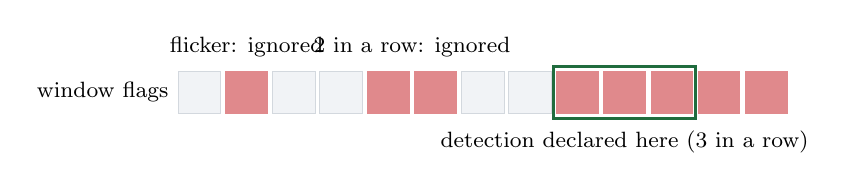
\begin{tikzpicture}[x=6mm,y=6mm]
  \foreach \i/\f in {0/0,1/1,2/0,3/0,4/1,5/1,6/0,7/0,8/1,9/1,10/1,11/1,12/1}{
    \ifnum\f=1 \fill[badred!60] (\i,0) rectangle (\i+0.9,0.9);
    \else \fill[panelgrey] (\i,0) rectangle (\i+0.9,0.9); \draw[linegrey] (\i,0) rectangle (\i+0.9,0.9); \fi
  }
  \draw[okgreen!70!black,very thick] (7.95,-0.1) rectangle (10.95,1.0);
  \node[font=\footnotesize,below] at (9.45,-0.15) {detection declared here (3 in a row)};
  \node[font=\footnotesize,above] at (1.45,1.0) {flicker: ignored};
  \node[font=\footnotesize,above] at (4.95,1.0) {2 in a row: ignored};
  \node[font=\footnotesize,left] at (0,0.45) {window flags};
\end{tikzpicture}}
\caption{The persistence rule. Isolated flags never count, either as
detections or as false alarms.}
\label{fig:persist}
\end{figure}

A detector that flickers above threshold one window in twenty has a
fine-looking detection rate and is unusable. The same rule counts false
alarms, so both numbers describe the same detector.

\section{The metrics}

\subsection{False alarms per day}
Measured on the held-out normal runs:
\begin{equation}
  \text{FAR} = \frac{\text{number of persistent excursions}}
                    {\text{normal time covered (s)}} \times 86\,400 .
\end{equation}
Operators experience alarms per shift, not per sample. The report also gives
the raw fraction of normal windows above threshold, which should be close to
$1-q$.

\subsection{Detection rate and delay}
For each faulty test run, the detection delay is the time from the declared
onset to the first persistent detection after it:
\begin{equation}
  \tau_d = t_\text{detect} - t_\text{onset} .
\end{equation}
Detection rate is the fraction of faulty runs detected; the report gives the
median delay overall and per fault mode. Incipient faults (long ramps) have
naturally longer delays.

\subsection{Isolation accuracy}
Once a fault has fully developed (ramp finished plus
\code{DEVELOPED_AFTER} $= 300$\,s), the most frequent top channel over the
remaining windows is compared with the channel physics names
(Chapter~\ref{ch:ml}). Judging earlier is wrong: fouling ramping over twenty
minutes is still a transient five minutes in, and the transient implicates
the controlled level rather than the downstream one.

If a run ends before the fault has developed, isolation is judged on the last
quarter of the post-onset data and the run is marked as not fully developed.

\subsection{Consistency}
For each mode, the fraction of runs whose top channel is that mode's most
common top channel. It needs no ground truth, so it is the only isolation
number available for sensor faults.

\begin{warn}[Why sensor faults are not scored for isolation]
In a closed loop, a level transmitter reading 25\,mm high is driven back to
setpoint by the controller: the reading looks perfect and the true level sits
25\,mm low. The signature appears everywhere \emph{except} the faulty
instrument, so ``the top channel should be \tg{LT101}'' is exactly backwards.
Scoring against that expectation would be scoring against a mistake.
\end{warn}

\section{Selecting the detector}

Each chosen method is fitted, calibrated and evaluated on the same split. The
one deployed is
\begin{equation}
  \arg\max_m \big(\text{detection rate}_m,\; -\text{FAR}_m\big)
\end{equation}
in lexicographic order: more detections wins, a tie goes to fewer false
alarms, and remaining ties go to the simpler model because the methods are
tried simplest first (z-score, PCA, isolation forest, autoencoder). A learned
detector that cannot beat PCA is not deployed just because it is newer.

\begin{figure}[htbp]
\centering
\scalebox{0.8}{%
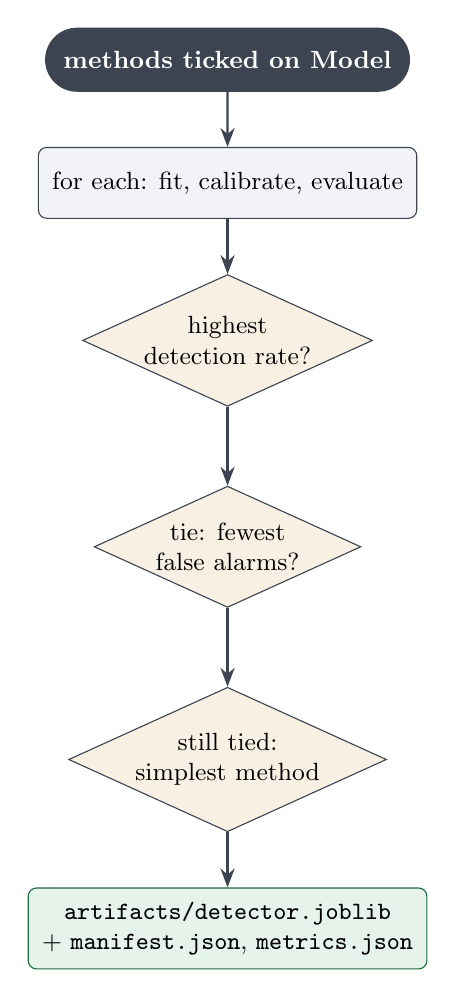
\begin{tikzpicture}[node distance=7mm]
  \node[term] (s) {methods ticked on \ui{Model}};
  \node[box,below=of s] (f) {for each: fit, calibrate, evaluate};
  \node[decision,below=of f] (d) {highest\\detection rate?};
  \node[decision,below=10mm of d] (t) {tie: fewest\\false alarms?};
  \node[decision,below=10mm of t] (u) {still tied:\\simplest method};
  \node[good,below=of u] (o) {\code{artifacts/detector.joblib}\\+ \code{manifest.json}, \code{metrics.json}};
  \draw[flow] (s) -- (f);
  \draw[flow] (f) -- (d);
  \draw[flow] (d) -- (t);
  \draw[flow] (t) -- (u);
  \draw[flow] (u) -- (o);
\end{tikzpicture}}
\caption{Model selection in \code{train_detector()}.}
\label{fig:select}
\end{figure}

\section{Reference results}

With the full dataset (58 one-hour runs: \code{python -m pyplant.ml.train
--duration 3600}) the project's reference numbers are:

\begin{center}
\begin{tabular}{@{}lcccc@{}}
\toprule
& Detection & Median delay & False alarms & Isolation \\
\midrule
PCA (MSPC baseline) & 83.3\% & 256\,s & 0 / day & 60\% \\
Autoencoder & \textbf{100\%} & \textbf{70\,s} & \textbf{0 / day} & \textbf{73\%} \\
\bottomrule
\end{tabular}
\end{center}

PCA detects only a third of the sensor bias and drift runs; the autoencoder
detects all of them. The physics channels do the isolation: leak runs point at
\tg{FLOW_IMBALANCE} 12 out of 12 times, pump wear at \tg{HEAD_RESIDUAL} 6/6
and stiction at \tg{OP_MINUS_ZT} 6/6. The raw window flag rate on normal runs
is 0.14\% and there are no persistent excursions. The z-score and isolation
forest detectors were added later; run them on your own dataset to place them
in this table. Smaller presets give noisier numbers.

\section{Reading the Model tab}

\begin{enumerate}
  \item The comparison table has one row per method: detection rate, median
        delay, false alarms per day, flagged normal windows and isolation.
        The deployed method is marked \emph{(selected)}.
  \item The per-mode table shows, for the selected method, the number of runs
        of each fault mode, the fraction detected, the median delay, the most
        common top channel and the channel physics expects.
  \item A low detection rate on one mode with a long delay usually means the
        fault was still ramping when the run ended; use longer runs.
  \item A non-zero false alarm rate means the threshold is too low for this
        data: raise the quantile (e.g.\ 0.999) or generate more normal runs.
\end{enumerate}

\chapter{Changing parameters}
\label{ch:params}

Parameters live in four places: the workbench forms, the workspace
\code{config.json}, the command-line flags of each service, and constants in
the code. This chapter says which is which, what each parameter does, and how
to change it safely.

\section{Where a parameter takes effect}

\begin{figure}[htbp]
\centering
\scalebox{0.8}{%
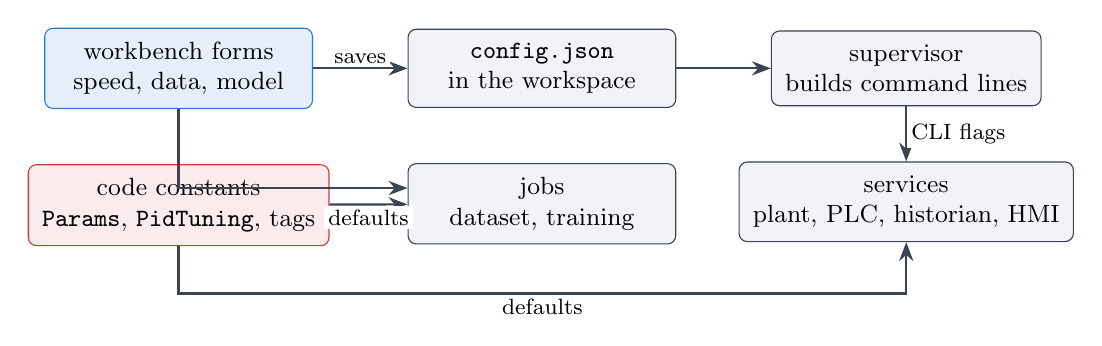
\begin{tikzpicture}[node distance=7mm and 12mm]
  \node[hot,minimum width=34mm] (ui) {workbench forms\\speed, data, model};
  \node[box,right=of ui,minimum width=34mm] (cfg) {\code{config.json}\\in the workspace};
  \node[box,right=of cfg,minimum width=34mm] (sup) {supervisor\\builds command lines};
  \node[box,below=of sup,minimum width=34mm] (svc) {services\\plant, PLC, historian, HMI};
  \node[box,below=of cfg,minimum width=34mm] (jobs) {jobs\\dataset, training};
  \node[bad,below=of ui,minimum width=34mm] (code) {code constants\\\code{Params}, \code{PidTuning}, tags};
  \draw[flow] (ui) -- node[lbl,above]{saves} (cfg);
  \draw[flow] (cfg) -- (sup);
  \draw[flow] (sup) -- node[lbl,right]{CLI flags} (svc);
  \draw[flow] (ui) |- ([yshift=2mm]jobs.west);
  \draw[flow] (code) -- node[lbl,below]{defaults} (jobs);
  \draw[flow] (code.south) -- ++(0,-6mm) -| node[lbl,pos=0.25,below]{defaults} (svc.south);
\end{tikzpicture}}
\caption{How a parameter reaches the code that uses it.}
\label{fig:paramflow}
\end{figure}

\begin{warn}[What is and is not wired]
The supervisor passes only \code{dt}, \code{speed}, \code{loop.setpoint} and
\code{loop.scan_period} from \code{config.json} to the services. The
\code{plant} section and \code{loop.kc}, \code{ti}, \code{td}, \code{tf} are
saved and read back, but the live services always use the code defaults of
\code{Params} and \code{PidTuning}. To experiment with plant parameters or
tuning, use the offline harness (Section~\ref{sec:offline}) or change the
defaults in the code.
\end{warn}

\section{The workspace configuration}

\code{config.json} is created on first start and rewritten atomically (to a
temporary file, then moved into place) whenever the workbench saves.

\begin{lstlisting}[style=sh]
{
  "name": "demo",
  "speed": 1.0,            // real-time factor of the live stack
  "dt": 0.05,              // s, plant integration step
  "ports": { "plant_modbus": 5400, "plant_control": 5401, "plc_modbus": 5402,
             "plc_opcua": 5403, "historian_api": 5404, "hmi": 5405 },
  "plant": { "area_tank1": 0.02, "area_tank2": 0.02, "height_max": 0.6,
             "pump_dp0": 60000.0, "pump_qmax": 0.000417,
             "valve_cv": 2.429e-06, "valve_rangeability": 30.0,
             "tau_valve": 2.0, "cda_12": 6.9e-05, "cda_2out": 9e-05 },
  "loop":  { "kc": 0.35, "ti": 72.0, "td": 0.0, "tf": 5.0,
             "setpoint": 300.0, "scan_period": 0.1 },
  "data":  { "duration": 3600.0, "magnitudes": 3, "repeats": 2,
             "normal_runs": 10, "window": 60, "stride": 10,
             "quantile": 0.995, "seed": 0 }
}
\end{lstlisting}
(JSON has no comments; they are added here for explanation.) Edit it with the
workbench stopped, or use the forms. A missing key falls back to its default.

\subsection{Runtime parameters}
\begin{center}
\begin{tabularx}{\textwidth}{@{}lllX@{}}
\toprule
Parameter & Default & Set from & Effect \\
\midrule
\code{speed} & 1.0 & \ui{Runtime} menu & real-time factor of plant and PLC (1, 2, 4, 10 or 20); saved when the stack starts \\
\code{dt} & 0.05\,s & \code{config.json} & RK4 integration step of the plant \\
\code{loop.setpoint} & 300\,mm & \code{config.json} & initial LIC101 setpoint; the operator can change it live \\
\code{loop.scan_period} & 0.10\,s & \code{config.json} & PLC scan period $T_s$ \\
\code{ports} & base 5400 & \code{--base-port} & six consecutive ports from the base \\
\bottomrule
\end{tabularx}
\end{center}

\begin{warn}[Speed on Windows]
At \code{speed} $s$ the PLC wakes every $T_s/s$ wall seconds. Windows timers
have a granularity of about 15.6\,ms, so above $4\times$ the scan period
($25$\,ms at $4\times$) approaches the timer resolution and scans overrun.
Use $\le 4\times$ on Windows; slow faults such as stiction need a few process
time constants (72\,s each) to develop.
\end{warn}

\subsection{Dataset parameters (Data tab)}
\begin{center}
\begin{tabular}{@{}lllll@{}}
\toprule
Parameter & Meaning & Quick & Standard & Thorough \\
\midrule
\code{duration} & seconds per run & 1200 & 3600 & 3600 \\
\code{magnitudes} & scale factors per fault & 1 & 3 & 5 \\
\code{repeats} & seeds per magnitude & 1 & 2 & 3 \\
\code{normal_runs} & minimum normal runs ($\ge3$) & 6 & 10 & 16 \\
\midrule
runs generated & & 14 & 58 & 136 \\
approximate time & & 1.5\,min & 4\,min & 10\,min \\
\bottomrule
\end{tabular}
\end{center}

Guidance: more magnitudes give the detector a wider view of fault severity;
more repeats make the evaluation numbers less noisy; more normal runs give a
better threshold and a more trustworthy false alarm rate. Duration must leave
time after onset (25--60\% of the run) for ramped faults to develop.

\subsection{Model parameters (Model tab)}
\begin{center}
\begin{tabularx}{\textwidth}{@{}llX@{}}
\toprule
Parameter & Default & Effect \\
\midrule
methods & all four & which detectors to fit and compare \\
\code{window} & 60 samples & longer windows see slower faults and smooth noise, at the cost of delay \\
\code{stride} & 10 samples & spacing of windows; smaller means finer delay resolution and more data \\
\code{quantile} & 0.995 & threshold quantile on calibration data; raise it (0.999) for fewer false alarms, lower it for faster detection \\
\code{seed} & 0 & split and model randomness (Python only) \\
\bottomrule
\end{tabularx}
\end{center}

\subsection{Fault parameters (Faults tab)}
\begin{center}
\begin{tabular}{@{}lll@{}}
\toprule
Kind & Starting magnitude & Unit \\
\midrule
\code{leak} & $5\times10^{-5}$ & m$^2$ effective leak area \\
\code{fouling} & 0.35 & fraction of flow area lost \\
\code{pump_wear} & 0.18 & fraction of head lost \\
\code{stiction} & 0.10 & deadband, fraction of stroke (slip default 0.04) \\
\code{sensor_bias} & 25 & tag units \\
\code{sensor_drift} & 1.5 & tag units per minute \\
\code{sensor_stuck} & none & \\
\code{sensor_noise} & 2.0 & $\sigma$ in tag units \\
\bottomrule
\end{tabular}
\end{center}
Sensor faults also take a tag (\tg{LT101}, \tg{LT102}, \tg{FT101},
\tg{FT102}, \tg{PT101} or \tg{ZT101}) and every fault takes a ramp in
seconds.

\section{Command-line options}
\label{sec:cli}

\subsection{Workbench}
\begin{lstlisting}[style=sh]
python -m pyplant.workbench.app [--workspace ./work/demo] [--base-port 5400]
                                [--host 127.0.0.1] [--port 8050] [--debug]
\end{lstlisting}

\subsection{Services}
These are the processes the supervisor starts; the \ui{Runtime} tab shows the
exact command line of each. They can be run by hand in four terminals.

\begin{center}
\begin{tabularx}{\textwidth}{@{}p{62mm}lX@{}}
\toprule
Flag & Default & Meaning \\
\midrule
\multicolumn{3}{@{}l}{\code{python -m pyplant.services.plant}} \\
\quad\code{--port} & 5020 & Modbus slave port \\
\quad\code{--control-port} & 0 & fault injection HTTP API; 0 disables \\
\quad\code{--dt} & 0.05 & integration step, s \\
\quad\code{--speed} & 1.0 & real-time factor \\
\quad\code{--start} & steady & \code{steady} or \code{empty} initial state \\
\quad\code{--no-noise} & off & disable instrument noise \\
\midrule
\multicolumn{3}{@{}l}{\code{python -m pyplant.services.plc}} \\
\quad\code{--plant-host}, \code{--plant-port} & 127.0.0.1, 5020 & where the plant is \\
\quad\code{--port} & 5021 & PLC Modbus server port \\
\quad\code{--opcua-port}, \code{--no-opcua} & 4840 & OPC UA server \\
\quad\code{--period} & 0.10 & scan period, s \\
\quad\code{--speed} & 1.0 & real-time factor \\
\quad\code{--setpoint} & 300 & initial setpoint, mm \\
\midrule
\multicolumn{3}{@{}l}{\code{python -m pyplant.services.historian}} \\
\quad\code{--endpoint} & & PLC OPC UA endpoint \\
\quad\code{--db} & pyplant.duckdb & database file \\
\quad\code{--publish-ms} & 200 & subscription publishing interval \\
\quad\code{--flush} & 1.0 & buffer flush period, s \\
\quad\code{--heartbeat} & 30 & maximum gap per tag, s \\
\quad\code{--api-port} & 0 & query API port; 0 disables \\
\midrule
\multicolumn{3}{@{}l}{\code{python -m pyplant.services.hmi}} \\
\quad\code{--endpoint} & & PLC OPC UA endpoint \\
\quad\code{--history} & & historian URL, or a DuckDB path \\
\quad\code{--port}, \code{--poll} & 8080, 0.5 & HTTP port, poll period (s) \\
\bottomrule
\end{tabularx}
\end{center}

\subsection{Training from the command line}
\begin{lstlisting}[style=sh]
python -m pyplant.ml.train --out artifacts --duration 3600 --magnitudes 3 \
       --repeats 2 --normal-runs 6 --window 60 --stride 10 --quantile 0.995 \
       --seed 0 [--reuse]
\end{lstlisting}
This fits PCA and the autoencoder; \code{--reuse} skips generation when
\code{dataset.parquet} already exists in \code{--out}.

\section{Code constants}

Some parameters are design decisions and live in code. Change them with care
and run \code{pytest} afterwards; the tests check most invariants.

\begin{center}
\begin{tabularx}{\textwidth}{@{}llX@{}}
\toprule
Constant & File & Meaning \\
\midrule
\code{Params} fields & \code{core/hybrid_tank.py} & plant geometry, pump, valve, orifices (Table~\ref{tab:params}) \\
\code{PidTuning} fields & \code{plc/pid.py} & $K_c$, $T_i$, $T_d$, $T_f$, limits, action \\
alarm limits & \code{tags.py} & \code{limits} on each tag: HI 500, HIHI 550, LOLO 50\,mm; PT HIHI 58\,kPa; FT LO 1\,L/min \\
deadbands & \code{plc/program.py} & 10\,mm, 2\,kPa, 0.5\,L/min \\
\code{MIN_FLOW_DELAY} & \code{plc/program.py} & 15\,s low-flow trip delay \\
\code{DEFAULT_NOISE} & \code{faults/scenarios.py} & instrument noise $\sigma$ per tag \\
\code{NORMAL_MOVES} & \code{faults/scenarios.py} & setpoint programme of the scenarios \\
\code{WINDOW}, \code{STRIDE} & \code{ml/features.py} & default window and stride \\
\code{PERSISTENCE} & \code{ml/evaluate.py} & consecutive windows for a detection (3) \\
\code{DEVELOPED_AFTER} & \code{ml/evaluate.py} & settling time before isolation is judged (300\,s) \\
\code{DATA_PRESETS}, \code{PRESETS} & \code{workbench/app.py} & dataset and fault presets in the UI \\
\bottomrule
\end{tabularx}
\end{center}

\section{Offline experiments with other parameters}
\label{sec:offline}

The fastest way to try a different plant or tuning is the offline harness: the
same PLC program, the same physics, no network, about 1900 times real time.

\begin{lstlisting}
from pyplant.core.hybrid_tank import Inputs, Params
from pyplant.plc.harness import OperatorPanel, PlcHarness, scheduled_setpoint
from pyplant.plc.pid import PidTuning
from pyplant.plc.program import Program
from pyplant.runners.base import Simulation
from pyplant.runners.fast import run

plant  = Params(area_tank1=0.03)                 # a wider tank 1
tuning = PidTuning(kc=0.6, ti=50.0)              # a more aggressive loop
harness = PlcHarness(program=Program(ts=0.1, tuning=tuning),
                     panel=OperatorPanel(setpoint=300.0))
sim = Simulation.at_steady_state(Inputs(0.662, True), params=plant,
                                 dt=0.05, control_period=0.1, policy=harness)
sim.policy = scheduled_setpoint(harness, [(0.0, 300.0), (60.0, 350.0)])
tr = run(sim, duration=600.0, log_period=1.0, extra=harness.tags)
df = tr.to_dataframe()            # LT101, LIC101_OP, ... one row per second
\end{lstlisting}

To generate scenario data with a different plant, pass \code{params} to the
scenario: \code{Scenario("wide", params=Params(area_tank1=0.03), ...)}. Note
that \code{run_scenario()} always uses the default \code{PidTuning}.

\subsection{Retuning after a plant change}
If you change the plant, re-identify $K$ and $\tau$ from an open-loop step
(Chapter~\ref{ch:tutorials}) and recompute the IMC settings:
\[
  K_c = \frac{\tau}{K\lambda}, \qquad T_i = \tau, \qquad
  \lambda \approx \tau/5 .
\]
A larger tank area increases $\tau$ roughly in proportion; the gain $K$
changes with the operating point because the valve and the drains are
non-linear.

\chapter{Extending the toolbox}
\label{ch:extend}

pyplant is meant to be changed. This chapter gives recipes for the four most
common extensions: a new tag, a new fault, a new detector and an online
inference service. In every case the rule is the same: change the single
source of truth, then let the tests tell you what else must follow.

\section{Adding a tag}

\begin{figure}[htbp]
\centering
\scalebox{0.8}{%
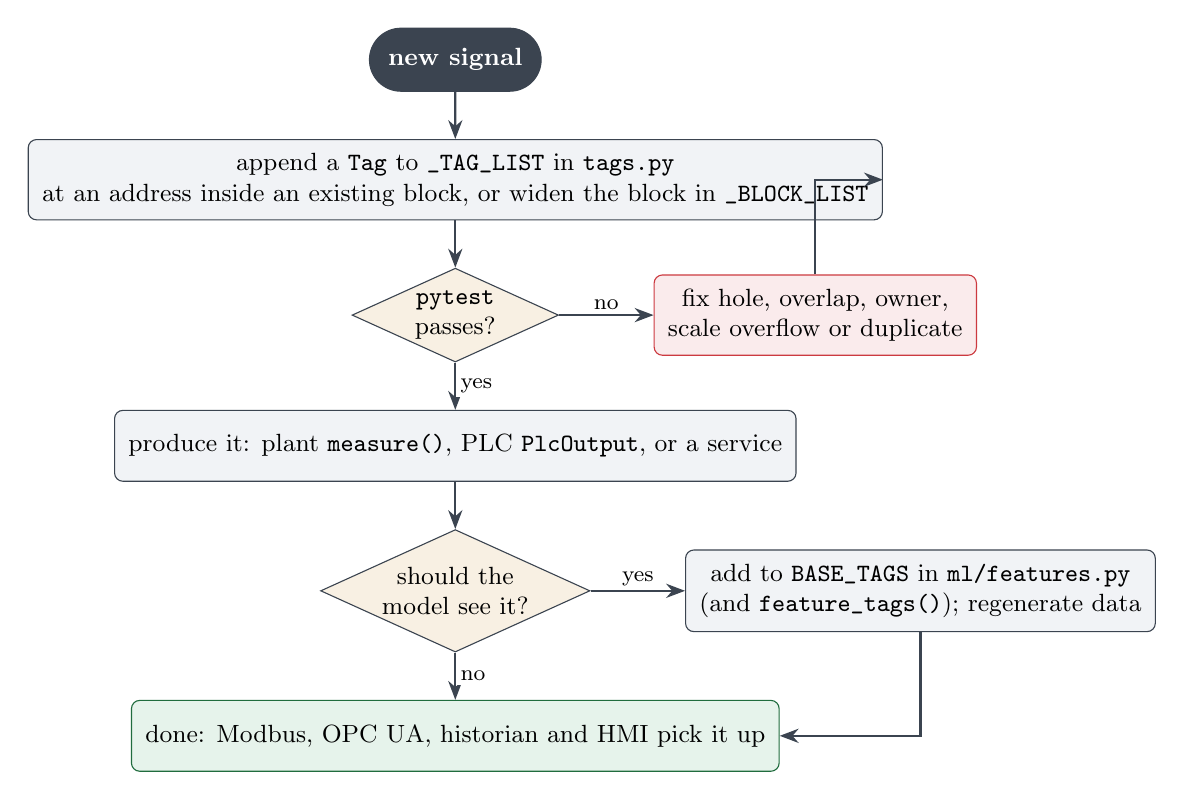
\begin{tikzpicture}[node distance=6mm]
  \node[term] (s) {new signal};
  \node[box,below=of s,minimum width=80mm] (a) {append a \code{Tag} to \code{_TAG_LIST} in \code{tags.py}\\at an address inside an existing block, or widen the block in \code{_BLOCK_LIST}};
  \node[decision,below=of a] (t) {\code{pytest}\\passes?};
  \node[bad,right=12mm of t] (fix) {fix hole, overlap, owner,\\scale overflow or duplicate};
  \node[box,below=of t,minimum width=80mm] (p) {produce it: plant \code{measure()}, PLC \code{PlcOutput}, or a service};
  \node[decision,below=of p] (m) {should the\\model see it?};
  \node[box,right=12mm of m] (f) {add to \code{BASE_TAGS} in \code{ml/features.py}\\(and \code{feature_tags()}); regenerate data};
  \node[good,below=of m] (done) {done: Modbus, OPC UA, historian and HMI pick it up};
  \draw[flow] (s) -- (a);
  \draw[flow] (a) -- (t);
  \draw[flow] (t) -- node[lbl,above]{no} (fix);
  \draw[flow] (fix) |- (a);
  \draw[flow] (t) -- node[lbl,right]{yes} (p);
  \draw[flow] (p) -- (m);
  \draw[flow] (m) -- node[lbl,above]{yes} (f);
  \draw[flow] (m) -- node[lbl,right]{no} (done);
  \draw[flow] (f) |- (done);
\end{tikzpicture}}
\caption{Adding a tag.}
\label{fig:addtag}
\end{figure}

Because every layer derives its I/O from the tag dictionary, a new tag
appears in the Modbus map, the OPC UA address space (with its unit and
range), the historian and the HMI's tag list without further code.

\begin{warn}[\code{DIAG_ORDER} is append-only]
\tg{TOP_CONTRIB} stores the top channel as an index into \code{DIAG_ORDER}.
Reordering it changes the meaning of every historised value. Only append.
\end{warn}

\section{Adding a fault}

\begin{enumerate}
  \item Decide the entry point (Chapter~\ref{ch:faults}). Either subclass
        \code{ParameterFault} and implement \code{apply()}, or subclass
        \code{SignalFault} and implement \code{corrupt()}. A new
        \emph{command} fault also
        needs a branch in \code{FaultSet.command()}, which today dispatches
        only \code{ValveStiction}.
  \item Set \code{kind} and \code{target} in \code{__post_init__} and return
        the magnitude from the \code{magnitude} property.
  \item Register it in \code{FAULT_KINDS} with the attribute a single
        magnitude number sets. The injection API and the Faults tab dropdown
        read this table.
  \item Add a starting magnitude and unit to \code{DEFAULT_MAGNITUDE} and
        \code{MAGNITUDE_UNITS} in \code{workbench/app.py}.
  \item Add a representative scenario to \code{library()} so it enters the
        dataset grid, and, if its magnitude attribute has a new name, teach
        \code{_scaled()} to scale it.
  \item If physics names the channel it should isolate to, add it to
        \code{EXPECTED_CHANNEL} in \code{ml/evaluate.py}.
  \item Write a test that the fault does what it claims, in
        \code{tests/test_faults.py}.
\end{enumerate}

\begin{lstlisting}
@dataclass
class OutletBlockage(ParameterFault):
    """Partial blockage of the tank 2 drain, as fraction of area lost."""
    loss: float = 0.3

    def __post_init__(self) -> None:
        super().__post_init__()
        self.kind, self.target = "outlet_blockage", "FE-2OUT"

    @property
    def magnitude(self) -> float:
        return self.loss

    def apply(self, p: Params, s: float) -> Params:
        return replace(p, cda_2out=p.cda_2out * (1.0 - self.loss * s))

FAULT_KINDS["outlet_blockage"] = (OutletBlockage, "loss")
\end{lstlisting}

\section{Adding a detector}

All detectors share the \code{Detector} base class, which provides
standardisation, calibration, health index, contributions and persistence.
A new method needs only two hooks:

\begin{description}
  \item[\code{_fit_core(Z)}] fit on standardised normal windows.
  \item[\code{_reconstruct(Z)}] return the reconstruction $\hat Z$. The score
        is then $\lVert Z - \hat Z\rVert^2$ and contributions come for free.
        A method with no reconstruction returns zeros and overrides
        \code{score()} instead, as the isolation forest does.
\end{description}

\begin{lstlisting}
from sklearn.covariance import EmpiricalCovariance

@dataclass
class MahalanobisDetector(Detector):
    """Hotelling-style distance using the full normal covariance."""
    cov: EmpiricalCovariance | None = None

    def __post_init__(self) -> None:
        self.kind = "mahalanobis"

    def _fit_core(self, Z):
        self.cov = EmpiricalCovariance().fit(Z)

    def _reconstruct(self, Z):
        return np.zeros_like(Z)          # contributions fall back to z^2

    def score(self, X):
        return self.cov.mahalanobis(self.scaler.transform(X))
\end{lstlisting}

Then add it to \code{METHODS} (label shown in the Model tab, in order from
simplest to most complex) and a branch in \code{make_detector()}. The Model
tab checklist and the selection rule pick it up automatically. Keep scores
positive with larger meaning worse, or the health index breaks.

\section{Adding an online inference service}

The \code{ML_RESULT} and \code{ML_ALARMS} blocks are reserved for a service
that scores the live plant. A minimal design:

\begin{figure}[htbp]
\centering
\scalebox{0.8}{%
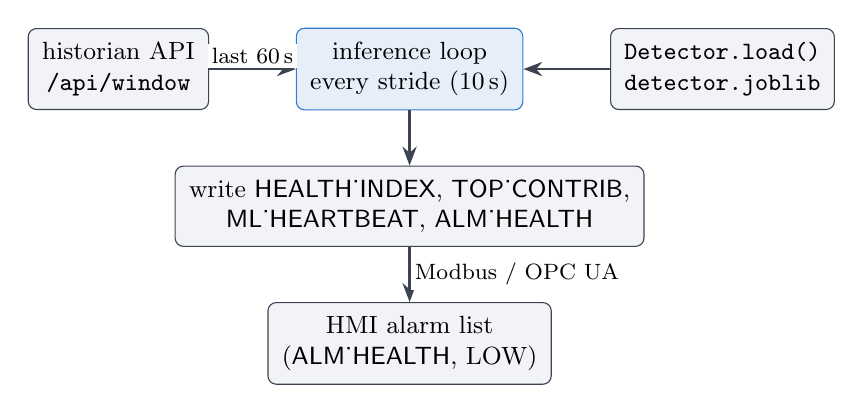
\begin{tikzpicture}[node distance=7mm and 11mm]
  \node[box] (h) {historian API\\\code{/api/window}};
  \node[hot,right=of h] (i) {inference loop\\every stride (10\,s)};
  \node[box,right=of i] (d) {\code{Detector.load()}\\\code{detector.joblib}};
  \node[box,below=of i] (w) {write \tg{HEALTH_INDEX}, \tg{TOP_CONTRIB},\\\tg{ML_HEARTBEAT}, \tg{ALM_HEALTH}};
  \node[box,below=of w] (hmi) {HMI alarm list\\(\tg{ALM_HEALTH}, LOW)};
  \draw[flow] (h) -- node[lbl,above]{last 60\,s} (i);
  \draw[flow] (d) -- (i);
  \draw[flow] (i) -- (w);
  \draw[flow] (w) -- node[lbl,right]{Modbus / OPC UA} (hmi);
\end{tikzpicture}}
\caption{Sketch of an inference service.}
\label{fig:inference}
\end{figure}

\begin{enumerate}
  \item Every stride, request the last \code{window} seconds of
        \code{BASE_TAGS} from the historian at 1\,Hz.
  \item Apply \code{add_derived()} and \code{windows()} to get one feature
        row.
  \item Compute \code{health()} and \code{top_channel()}; map the channel to
        its \code{DIAG_ORDER} index (0 for derived channels or no dominant
        tag).
  \item Write the results to the \code{ML_RESULT} block on the PLC's Modbus
        server; increment \tg{ML_HEARTBEAT} so a stalled service is visible.
  \item Set \tg{ALM_HEALTH} after the same persistence rule used in
        evaluation (three consecutive windows above 50).
  \item Add it to \code{SERVICES} in \code{workbench/supervisor.py} after
        the historian.
\end{enumerate}

Remember that historian timestamps are wall clock: at \code{speed} $>1$, ask
for \code{window / speed} wall seconds.

\section{Testing}

Run the whole suite from the project root:
\begin{lstlisting}[style=sh]
python -m pytest -q              # about 370 tests
python -m pytest tests/test_ml.py -q -k detector
\end{lstlisting}
The tests encode the invariants this manual describes: codec round trips,
registry rules, conservation of mass, step independence, PID properties,
drift-free scheduling, alarm state transitions, write guards, stiction
cycles, split leakage and the detector interface. A change that breaks one of
them has usually broken an assumption somewhere else too.

\chapter{API reference}
\label{ch:api}

Every service has a small JSON-over-HTTP API, and every layer has a Python
API. This chapter lists both. Ports are the workbench defaults with base
5400 (Table~\ref{tab:ports}); add your own base offset if you changed it.

\section{Plant control API (port 5401)}

Fault injection for the live plant. It is deliberately separate from anything
the control system can see: an operator, the HMI or a diagnosis model must
not be able to find out that a fault was injected except by observing the
plant.

\begin{center}
\begin{tabularx}{\textwidth}{@{}llX@{}}
\toprule
Method & Path & Purpose \\
\midrule
GET & \code{/api/faults} & plant time, available kinds, real faults, instrument noise entries, ids active now \\
POST & \code{/api/fault} & inject a fault; returns its label; 422 if invalid \\
DELETE & \code{/api/fault/{id}} & remove one fault; 404 if unknown \\
DELETE & \code{/api/faults} & remove all real faults, keep instrument noise \\
GET & \code{/api/truth} & current label, true and reported measurements \\
\bottomrule
\end{tabularx}
\end{center}

The \code{POST /api/fault} body:
\begin{center}
\begin{tabular}{@{}lll@{}}
\toprule
Field & Default & Meaning \\
\midrule
\code{kind} & required & one of \code{FAULT_KINDS} \\
\code{id} & \code{<kind>_<t>} & unique id \\
\code{magnitude} & kind default & value of the kind's magnitude attribute \\
\code{tag} & \tg{LT101} & sensor faults only \\
\code{delay} & 0 & plant seconds from now until onset \\
\code{duration} & none & plant seconds until the fault ends \\
\code{ramp} & 0 & seconds to full magnitude \\
\bottomrule
\end{tabular}
\end{center}

\begin{lstlisting}[style=sh]
# PowerShell
Invoke-RestMethod -Method Post -Uri http://127.0.0.1:5401/api/fault `
  -ContentType application/json `
  -Body '{"kind":"leak","magnitude":5e-5,"ramp":300}'
Invoke-RestMethod http://127.0.0.1:5401/api/truth

# bash / curl
curl -X POST localhost:5401/api/fault -H "Content-Type: application/json" \
     -d '{"kind":"sensor_bias","tag":"LT101","magnitude":25}'
curl -X DELETE localhost:5401/api/faults
\end{lstlisting}

\section{Historian query API (port 5404)}

\begin{center}
\begin{tabularx}{\textwidth}{@{}llX@{}}
\toprule
Method & Path & Purpose \\
\midrule
GET & \code{/api/health} & row count, tag count, time span, collector statistics \\
GET & \code{/api/window} & query \code{tags=A,B}, \code{seconds=300}, \code{freq=1}: the last \code{seconds} of the listed tags on a regular grid (LOCF); \code{null} where no value yet; 404 for unknown tags \\
GET & \code{/api/latest} & query \code{tags=A,B}: most recent good value per tag (all tags if omitted) \\
\bottomrule
\end{tabularx}
\end{center}

\section{HMI API (port 5405)}

\begin{center}
\begin{tabularx}{\textwidth}{@{}llX@{}}
\toprule
Method & Path & Purpose \\
\midrule
GET & \code{/} & the operator page \\
GET & \code{/api/state} & connected flag, last update, all values, active alarm list, alarm summary, poll and error counts \\
GET & \code{/api/tags} & tag dictionary: description, unit, span, kind, writable \\
GET & \code{/api/trend} & query \code{tags}, \code{seconds}, \code{freq}: trend data via the historian; 503 if none \\
POST & \code{/api/setpoint} & body \code{{"value": 320}}: write \tg{LIC101_SP} \\
POST & \code{/api/manual} & body \code{{"value": 70}}: write \tg{LIC101_MAN_OP} \\
POST & \code{/api/mode} & body \code{{"auto": false}}: auto or manual \\
POST & \code{/api/pump} & body \code{{"start": true}}: pump start request \\
POST & \code{/api/reset} & pulse alarm and interlock reset \\
POST & \code{/api/alarms/ack} & body \code{{"tag": "ILK_PMP101"}}: acknowledge one alarm; \code{null} acknowledges all \\
POST & \code{/api/alarms/shelve} & body \code{{"tag": ..., "minutes": 30, "reason": ...}}; at most 8\,h \\
POST & \code{/api/alarms/unshelve} & body \code{{"tag": ...}}: return a shelved alarm to service \\
\bottomrule
\end{tabularx}
\end{center}

Writes are guarded (404 unknown tag, 403 not writable, 422 out of span, 503
not connected), as described in Chapter~\ref{ch:scada}.

\section{Industrial protocols}

\begin{description}
  \item[Modbus TCP, plant (5400)] holding registers 0--5 (measurements),
        coil 0 (pump running); the PLC writes HR 10 (valve) and coil 10
        (pump).
  \item[Modbus TCP, PLC (5402)] the full tag map of Appendix~\ref{app:tags}.
        Any Modbus client can read it; the operator blocks are writable.
  \item[OPC UA, PLC (5403)] endpoint
        \\ \code{opc.tcp://127.0.0.1:5403/pyplant/}, \\ nodes under
        \code{Plant/Unit1}, \code{PLC/LIC101}, \code{PLC/Commands},
        \code{PLC/Alarms}, \code{PLC/Diagnostics}, with engineering units and
        ranges. Browse it with any OPC UA client, e.g.\ UaExpert.
\end{description}

\section{Python API}

\subsection{Tags}
\begin{lstlisting}
from pyplant.tags import tag, tags_in, TAGS, BLOCKS
lt = tag("LT101")
lt.encode(432.7)        # 4327 on the wire
lt.decode(4327)         # 432.7
lt.path                 # 'Plant/Unit1/LT101'
lt.limits.hihi          # 550.0
tags_in("PLANT_MEAS")   # the six tags polled in one read
\end{lstlisting}

\subsection{Plant physics}
\begin{lstlisting}
import numpy as np
from pyplant.core.hybrid_tank import Params, Inputs, step, steady_state, measure
p, u = Params(), Inputs(valve_cmd=0.662, pump_on=True)
x = steady_state(u, p)               # analytic equilibrium
x = step(x, u, p, dt=0.05)           # one RK4 step
measure(x, u, p)                     # {'LT101': 300.3, 'FT101': 10.05, ...}
\end{lstlisting}

\subsection{Simulation and runners}
\begin{lstlisting}
from pyplant.runners.base import Simulation, piecewise
from pyplant.runners.fast import run, settle
sim = Simulation.at_steady_state(Inputs(0.60, True), policy=piecewise([
    (0.0, Inputs(0.60, True)), (300.0, Inputs(0.70, True))]))
tr = run(sim, duration=1800.0, log_period=1.0)
tr.to_dataframe()
\end{lstlisting}

\subsection{Main modules}
\begin{center}
\begin{tabularx}{\textwidth}{@{}lX@{}}
\toprule
Object & Purpose \\
\midrule
\code{plc.pid.PID}, \code{PidTuning} & velocity PID; \code{step()}, \code{track()} \\
\code{plc.program.Program} & one scan: \code{execute(PlcInput) -> PlcOutput} \\
\code{plc.harness.PlcHarness} & program as a simulation policy, no network \\
\code{plc.scan.ScanEngine} & real-time scan cycle over an \code{IOLink} \\
\code{clock.Ticker} & drift-free periodic wake-ups \\
\code{faults.model} & fault classes, \code{FaultSet}, \code{build_fault} \\
\code{faults.scenarios} & \code{Scenario}, \code{run_scenario}, \code{library}, \code{grid} \\
\code{hist.db.Historian} & DuckDB store; \code{write}, \code{get_window}, \code{covered_span} \\
\code{hmi.alarms.AlarmManager} & ISA-18.2 alarm list \\
\code{ml.dataset} & \code{build}, \code{default_dataset}, \code{split_scenarios}, \code{windowed} \\
\code{ml.features} & \code{add_derived}, \code{windows}, \code{WindowSpec} \\
\code{ml.detector} & detectors, \code{make_detector}, \code{METHODS} \\
\code{ml.evaluate.evaluate} & \code{Report} with FAR, delay, isolation \\
\code{workbench.workspace.Workspace} & config, run log, paths \\
\code{workbench.supervisor.Supervisor} & start and stop the four services \\
\bottomrule
\end{tabularx}
\end{center}

\chapter{Troubleshooting}
\label{ch:trouble}

\begin{figure}[htbp]
\centering
\scalebox{0.8}{%
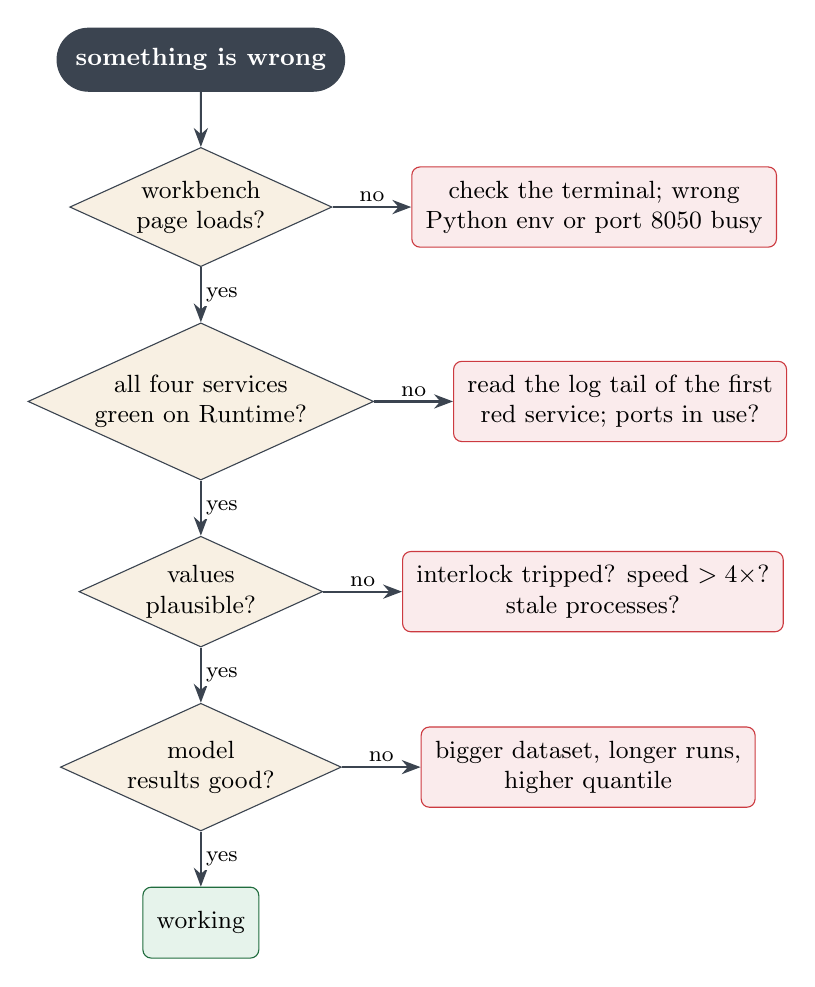
\begin{tikzpicture}[node distance=7mm and 10mm]
  \node[term] (s) {something is wrong};
  \node[decision,below=of s] (w) {workbench\\page loads?};
  \node[bad,right=of w] (w1) {check the terminal; wrong\\Python env or port 8050 busy};
  \node[decision,below=of w] (st) {all four services\\green on Runtime?};
  \node[bad,right=of st] (st1) {read the log tail of the first\\red service; ports in use?};
  \node[decision,below=of st] (v) {values\\plausible?};
  \node[bad,right=of v] (v1) {interlock tripped? speed $>4\times$?\\stale processes?};
  \node[decision,below=of v] (m) {model\\results good?};
  \node[bad,right=of m] (m1) {bigger dataset, longer runs,\\higher quantile};
  \node[good,below=of m] (ok) {working};
  \draw[flow] (s) -- (w);
  \draw[flow] (w) -- node[lbl,above]{no} (w1);
  \draw[flow] (w) -- node[lbl,right]{yes} (st);
  \draw[flow] (st) -- node[lbl,above]{no} (st1);
  \draw[flow] (st) -- node[lbl,right]{yes} (v);
  \draw[flow] (v) -- node[lbl,above]{no} (v1);
  \draw[flow] (v) -- node[lbl,right]{yes} (m);
  \draw[flow] (m) -- node[lbl,above]{no} (m1);
  \draw[flow] (m) -- node[lbl,right]{yes} (ok);
\end{tikzpicture}}
\caption{Where to look first.}
\label{fig:trouble}
\end{figure}

\section{Installation and start-up}

\paragraph{\code{SyntaxError} or \code{ImportError: StrEnum} at start.}
The project needs Python 3.11 or later: the alarm module uses
\code{enum.StrEnum}, although \code{pyproject.toml} still says 3.10. The base
interpreter on many machines
is older; activate the project environment first
(\code{conda activate pyplant}) or call its \code{python.exe} directly.

\paragraph{\code{pymodbus} errors such as unexpected keyword
\code{slave}.} The Modbus layer is written against pymodbus 3.8. Reinstall
the pinned version: \code{pip install "pymodbus>=3.8,<3.9"}.

\paragraph{``ports already in use by something else''.} Another stack, or
leftover processes from a crashed session, hold the ports. Start with a
different base (\code{--base-port 5500}) or stop the leftovers. On Windows:
\begin{lstlisting}[style=sh]
Get-CimInstance Win32_Process |
  Where-Object { $_.CommandLine -match 'pyplant\.(services|workbench)' } |
  ForEach-Object { Stop-Process -Id $_.ProcessId -Force }
\end{lstlisting}
On Linux or macOS: \code{pkill -f pyplant.services}.

\paragraph{A service turns red right after start.} The Runtime tab shows the
last lines of its log, and the full log is in \code{<workspace>/jobs/<name>.log}.
Services start in order (plant, PLC, historian, HMI), so fix the first red one.

\section{The live stack}

\paragraph{The page is slow or callbacks lag.} When a service is down, each
request to it would wait for the connection to be refused, which takes about
2\,s on Windows. The workbench connects with a 0.5\,s timeout and then reports
the service as down for 2.5\,s without retrying. If the page is still slow,
stop the stack cleanly and restart it.

\paragraph{\tg{SCAN_OVERRUNS} keeps rising, the loop is sluggish.} The speed
is too high for the operating system's timer. Use $\le4\times$ on Windows.

\paragraph{The level drops to zero and the pump is off.} The interlock has
tripped, usually on low flow after the valve was driven shut (manual output
0\%) or after a large leak. Remove the cause, then press \ui{Reset} on the
HMI. Acknowledging the alarm alone does not reset the trip.

\paragraph{The HMI says ``not connected''.} The HMI talks to the PLC over OPC
UA. Check that the PLC service is green and that port 5403 is listening; the
HMI reconnects on its own once the PLC is up.

\paragraph{Trends are empty for the first seconds.} The historian has to
receive a value of every requested tag before a window is complete. Wait a few
seconds after start, or longer for quiet tags (heartbeat 30\,s).

\paragraph{I injected a fault and nothing happens.} Often correct: integral
action holds the level on setpoint (Section~\ref{sec:masking}). Watch the
controller output and \code{GET /api/truth}. Slow faults (fouling, wear with
ramps, stiction) need several minutes of plant time.

\section{Data and models}

\paragraph{``need at least three normal runs''.} Raise \ui{Normal runs} on
the Data tab to 3 or more (6 is a sensible minimum).

\paragraph{``there is no dataset yet''.} Generate one on the Data tab before
training. Datasets are stored in the workspace and survive restarts.

\paragraph{\code{PermissionError} on a job state file (Windows).} Antivirus or
the indexer briefly locks a file the job is rewriting. The job runner retries
for up to 0.2\,s; if it persists, exclude the workspace directory from
real-time scanning.

\paragraph{Detection rate is low for one fault mode.} Check the per-mode
table: if the fault ramps for 20 minutes and runs are 20 minutes long, it never
develops. Use 3600\,s runs. Low-magnitude variants in the grid are meant to be
hard.

\paragraph{False alarms on normal runs.} Increase the quantile (0.999), add
normal runs, or increase the window to smooth noise.

\paragraph{The autoencoder is worse than PCA.} With little data this is
expected and the selection rule will deploy PCA. Use the Standard or Thorough
preset.

\section{Starting over}

Deleting the workspace directory is always safe; the next start recreates it
with defaults. From Python, \code{Workspace(path).reset()} deletes data,
artefacts, history and the run log but keeps the configuration.


\appendix
\chapter{Reference}

\section{Tag list}
\label{app:tags}

HR = holding register, C = coil. Scale is the integer factor on the wire.

{\small\setlength{\tabcolsep}{4pt}
\begin{longtable}{@{}llllllll@{}}
\toprule
Tag & Description & Owner & Table & Addr & Unit & Span & Scale \\
\midrule
\endhead
\multicolumn{8}{@{}l}{\textit{Plant measurements (block \code{PLANT_MEAS}, \code{PLANT_STATUS})}} \\
\tg{LT101} & tank 1 level & PLANT & HR & 0 & mm & 0--600 & 10 \\
\tg{LT102} & tank 2 level & PLANT & HR & 1 & mm & 0--600 & 10 \\
\tg{FT101} & pump discharge flow & PLANT & HR & 2 & L/min & 0--20 & 100 \\
\tg{FT102} & tank 2 outlet flow & PLANT & HR & 3 & L/min & 0--20 & 100 \\
\tg{PT101} & pump discharge pressure & PLANT & HR & 4 & kPa & 0--100 & 100 \\
\tg{ZT101} & valve stem position & PLANT & HR & 5 & \% & 0--100 & 100 \\
\tg{PMP101_RUN} & pump running & PLANT & C & 0 & & & \\
\multicolumn{8}{@{}l}{\textit{Actuator commands (\code{PLC_CMD}, \code{PLC_CMD_BITS})}} \\
\tg{FCV101_OP} & valve command & PLC & HR & 10 & \% & 0--100 & 100 \\
\tg{PMP101_CMD} & pump start command & PLC & C & 10 & & & \\
\multicolumn{8}{@{}l}{\textit{Operator (\code{OPER_SP}, \code{OPER_CMD}); writable}} \\
\tg{LIC101_SP} & setpoint & OPER & HR & 20 & mm & 0--600 & 10 \\
\tg{LIC101_MAN_OP} & manual output demand & OPER & HR & 21 & \% & 0--100 & 100 \\
\tg{LIC101_AUTO} & loop in automatic & OPER & C & 11 & & & \\
\tg{CMD_ALM_RESET} & alarm and interlock reset & OPER & C & 12 & & & \\
\tg{CMD_PMP101_START} & pump start request & OPER & C & 13 & & & \\
\multicolumn{8}{@{}l}{\textit{Faceplate readback (\code{PLC_FACE})}} \\
\tg{LIC101_PV} & process value & PLC & HR & 22 & mm & 0--600 & 10 \\
\tg{LIC101_OP} & controller output & PLC & HR & 23 & \% & 0--100 & 100 \\
\tg{LIC101_ERR} & control error & PLC & HR & 24 & mm & $\pm$600 & 10 \\
\multicolumn{8}{@{}l}{\textit{Diagnostics (\code{PLC_DIAG})}} \\
\tg{SCAN_MS} & scan time & PLC & HR & 30 & ms & 0--1000 & 10 \\
\tg{SCAN_OVERRUNS} & overrun count & PLC & HR & 31 & count & 0--30000 & 1 \\
\tg{PLC_HEARTBEAT} & heartbeat counter & PLC & HR & 32 & count & 0--30000 & 1 \\
\multicolumn{8}{@{}l}{\textit{Alarms and interlocks (\code{PLC_ALARMS})}} \\
\tg{ALM_LT101_HI} & tank 1 level high & PLC & C & 20 & & & \\
\tg{ALM_LT101_LOLO} & tank 1 level low low & PLC & C & 21 & & & \\
\tg{ALM_PT101_HIHI} & pressure high high & PLC & C & 22 & & & \\
\tg{ILK_PMP101} & pump interlock latched & PLC & C & 23 & & & \\
\multicolumn{8}{@{}l}{\textit{Inference results (\code{ML_RESULT}, \code{ML_ALARMS}); reserved}} \\
\tg{HEALTH_INDEX} & model health index & ML & HR & 40 & \% & 0--100 & 100 \\
\tg{TOP_CONTRIB} & top contributing tag & ML & HR & 41 & enum & 0--64 & 1 \\
\tg{ML_HEARTBEAT} & inference heartbeat & ML & HR & 42 & count & 0--30000 & 1 \\
\tg{ALM_HEALTH} & health index degraded & ML & C & 30 & & & \\
\bottomrule
\end{longtable}
}

Print the live list and block plan with \code{python -m pyplant.tags}.

\section{File layout}

\begin{lstlisting}[style=sh]
pyplant/
  tags.py                 tag registry, codec, block plan
  clock.py                drift-free Ticker
  core/hybrid_tank.py     plant physics (pure functions, SI units)
  runners/base.py         Simulation stepper, zero-order hold, policies
  runners/fast.py         non-real-time driver, Trajectory, settle
  runners/realtime.py     real-time plant task
  plc/pid.py              velocity-form PID
  plc/program.py          image tables, alarms, interlocks, timers
  plc/harness.py          in-process PLC wiring for datasets and experiments
  plc/scan.py             scan engine, IOLink, diagnostics
  net/store.py, link.py   Modbus datastore, TagServer, TagClient
  net/opcua.py            OPC UA address space, server view, client
  services/plant.py       plant node (Modbus slave + fault API)
  services/plc.py         soft PLC node (Modbus client/server + OPC UA)
  services/historian.py   OPC UA collector + query API
  services/hmi.py         HMI process
  hist/db.py              DuckDB store, LOCF windows
  hmi/alarms.py           ISA-18.2 alarm state machine
  hmi/app.py, page.html   HMI API and operator page
  faults/model.py         fault objects, FaultSet, FAULT_KINDS
  faults/scenarios.py     scenario library, grid, run_scenario
  ml/features.py          windows, statistics, derived channels
  ml/dataset.py           generation, Parquet, scenario-level split
  ml/detector.py          z-score, PCA, isolation forest, autoencoder
  ml/evaluate.py          false alarms, delay, isolation
  ml/train.py             command-line training pipeline
  workbench/app.py        Dash workbench
  workbench/workspace.py  configuration, run log, paths
  workbench/supervisor.py start and stop the services
  workbench/jobs.py       background jobs
  workbench/tasks.py      dataset, training and quick-start tasks
  workbench/clients.py    HTTP clients for the services
tests/                    pytest suite
manual/                   this manual
\end{lstlisting}

\section{Glossary}

\begin{description}[itemsep=1pt]
  \item[Anti-windup] Preventing the integral term from accumulating while
        the actuator is saturated.
  \item[ASOF join] A join that matches each row to the latest row of another
        table at or before its time; used for LOCF resampling.
  \item[Autoencoder] A neural network trained to reproduce its input through
        a narrow bottleneck.
  \item[Bumpless transfer] Switching between manual and auto without a jump
        in controller output.
  \item[Contribution] A channel's share of a window's anomaly score.
  \item[EURange] OPC UA property giving a variable's engineering range.
  \item[FAR] False alarm rate, here persistent alarms per day on normal
        data.
  \item[Health index] Anomaly score mapped to 0--100 with the threshold at
        50.
  \item[HMI] Human--machine interface, the operator's screen.
  \item[Hysteresis] Different set and clear thresholds to stop chattering.
  \item[IMC] Internal model control, a model-based tuning method.
  \item[Image table] A PLC's snapshot of inputs or outputs for one scan.
  \item[Interlock] Protective logic that forces a safe state and latches.
  \item[ISA-18.2] The standard for alarm management in process industries.
  \item[Isolation forest] Tree ensemble that scores how easily a point is
        isolated by random splits.
  \item[LOCF] Last observation carried forward.
  \item[Modbus TCP] Simple register-based field protocol.
  \item[MSPC] Multivariate statistical process control.
  \item[OPC UA] Information-model protocol with typed, browsable nodes.
  \item[OP, PV, SP] Controller output, process value, setpoint.
  \item[P\&ID] Piping and instrumentation diagram.
  \item[PCA] Principal component analysis.
  \item[Persistence] Consecutive flagged windows required for a detection.
  \item[PLC] Programmable logic controller.
  \item[RK4] Fourth-order Runge--Kutta integration.
  \item[SCADA] Supervisory control and data acquisition.
  \item[Scan cycle] Read inputs, execute logic, write outputs, repeat.
  \item[Shelving] Temporary, expiring suppression of an alarm.
  \item[SPE ($Q$)] Squared prediction error off the PCA subspace.
  \item[Stiction] Static friction in a valve: sticking, then slipping.
  \item[TON] On-delay timer.
  \item[Velocity form] PID computing the change in output each scan.
  \item[ZOH] Zero-order hold; output held constant between samples.
\end{description}


\end{document}
